%!TEX root = ../report.tex

\chapter{Results}
\label{chap:results}

In this section the evaluation results of all three architectures and related best hyperparameter search results and detailed analysis is presented. Also the architectures are compared to each other based on the prediction on test data.

\section{DenseNet-Siamese Network}
How the search for best hyperparameters for the DenseNet-Siamese are designed and corresponding results are presented in the following section. 

\subsection{DenseNet-Siamese Hyperparameters To Be Evaluated}
The whole search space is divided into smaller blocks such as hyperparameters for DenseNet, hyperparameters for Siamese and others.
\subsubsection{Hyperparameters Of DenseNet}
\label{hyperDenseNet}
Layers per block defines both the depth of the DenseNet, which is automatically calculated and also defines the number of dense blocks. Besides growth rate, reduction, bottleneck, number of filters (nb\_filter), pooling,
include top, dropout, subsample initial block and weights are the most of the hyperparameters needed to be defined to instantiate a DenseNet. While some of this values will be fixed for all the evaluation, some needs to be 
chosen from a possible set of value, which could be infinite as well. 

\subsubsection{Hyperparameters Of Siamese Network}
Rest of the Siamese network that serve as decision network that connects the two DenseNet branches have the hyperparameters as follows. FC layer output size, dropout probability value.


\subsubsection{Other hyperparameters}
Apart from the aforementioned ones there are other general hyperparameters such as learning rate, batch size for training and optimizer. 
In the following part of the report it is described that how the whole search space is divided into smaller, well defined parts. The results are visualized with help of charts and tables to help in decision making.

\subsection{DenseNet Growth Rate And Layers Per Block Analysis}
 Most important part of this network is the feature extraction capability of the DenseNet branches. The overall performance of the network depends on it. So the first focus of the hyperparameter search is to find out the 
 main parameters defining the DenseNet architecture. The overall search space for this could be very big or even infinite. So for the first evaluation we define a coarse search space. With hope to find a best performing 
 parameter configuration or at least narrow down the search space.
 Layers per block are chosen among 2, 3, 4, 5, 6. For single dense block evaluation goes up-to 12 layers. More than that(14) causes memory to run out as the size gets too big 
 for the cluster gpu memory(16GB). Each network has been evaluated for growth rates of 6, 12, 18, 24, 30, 36. Different dense block sizes of 1, 2, 3, 4. The parameters compression/reduction and bottleneck are set 0.5 and 'True' respectively.
 Both this parameters control the compactness of the model and help reducing the parameter required, hence in theory, making it possible to evaluate much bigger networks without running into memory shortage issue. 
 The network that is being evaluated here are named DenseNet-BC by authors, i.e DenseNet with bottleneck and compression. 
 
 There are other parameters but number of dense block, growth rate and layers per block and reduction ratio are the main parameters which controls the architecture and parameter size of the network the most.
 The goal of this focused search is to narrow down the overall search space from the DenseNet parameters perspective. For more fine grained analysis the compression and bottleneck parameters will also be evaluated. 
 
 DenseNet parameters number of filter (nb\_filter) value are fixed at 16 for this search. The parameter classes are set to 2, which represents 1 for matching and 0 for not-matching pairs. 96, 96 is the input image dimensions. 
 And it is single channel. So depending on local setting of the keras, 'channel-first' or 'channel-last' suitable input shape is chosen automatically as (1, 96, 96) or (96, 96, 1) respectively.
 
 Subsample initial block enables the sub sampling of the initial input image to reduce the computation cost. The value is set to 'True'. The DenseNet parameter 'weights' value is set to 'None' to ensure that previously 
 trained weights are not used. The decision network is not required for the branches as Siamese provides that, the value for parameter include top is set to 'False'.
 The learning rate used for the test is 2E-4. As a regularization measurement dropout probability value for DenseNet used as 0.2 to handle over-fitting. To ensure the grid search is effective, too much regularization is not good, 
 as it can be restricting the overall evaluation at times. Epochs can be different for each architectures to ensure that the networks are able to achieve good training accuracy. But networks should not be over training, so the 
 choice of epoch is selected after multiple manual trials for each set of network configuration in the search space. From the Siamese side of the parameters, after concatenating the DenseNet branch output feature maps, 
 the combined features then passed through a fully-connected layer of 512 output size, which is followed by 'ReLU' activation and batch normalization (BN) and then a dropout layer with probability 0.5 has been added to ensure better 
 generalization. 
 Some of this values could have been further evaluated, how ever the values are obtained after lot of manual tuning and assured to be a decent starting point. 'Flatten' is used as pooling at the end of the DenseNet branches. Instead
 of the global average pooling from the original implementation. This causes increase in parameters overall though. Because with 'flatten' the multidimensional feature map at the end of DenseNet branch is just flattened. Where as in
 global average pooling \cite{lin2013network}, apart from the channel other dimensions are simply collapsed. But it is found that with 'flatten' the network is able to achieve much higher training accuracy and generalization too for 
 this network. Binary cross entropy loss function with 'Sigmoid' activation function used for the binary classification, this final layer acts as the binary classifier. In all the cases the networks are trained from scratch. 
%TODO really need a network structure here

\subsubsection{Growth Rate And Layers Per Block Search Setup Summary}
The overall search space is summarized in the section below.
\subsubsection{Fixed Hyperparameters}
Other hyperparameters that are needed to instantiate the DenseNet are set to fixed values \ref{table:architecture_gr_densenet_siamese} after manual trials, in order to focus on the layers per block and growth rate parameters.

\begin{table}[ht]
\centering
\caption{Fixed hyperparameter values for the evaluation setup.}
\resizebox{\textwidth}{!}
{\begin{tabular}{|l c| l c| l c|} 
 \hline\hline
 \rowcolor{lightgrey}
 \multicolumn{1}{|c}{\textbf{Name}} & \multicolumn{1}{c|}{\textbf{Value}} & \multicolumn{1}{c}{\textbf{Name}} & \multicolumn{1}{c|}{\textbf{Value}} & \multicolumn{1}{c}{\textbf{Name}} & \multicolumn{1}{c|}{\textbf{Value}} \\ [0.5ex] 
 \hline
 Number of filter & 16 & Subsample initial block & 'True' & Weights & 'None'\\
 \hline
 Dropout rate & 0.2 & Include top & 'False' & Compression & 0.5\\
 \hline
 Bottleneck & 'True' & Pooling & 'flatten' & Transition pooling & 'max' \\
 \hline
 Siamese FC output & 512 & Siamese dropout & 0.5 & Optimizer & 'adam' \\
 \hline
 Learning rate & 2E-4 & & & & \\
 \hline \hline
\end{tabular}}
\label{table:architecture_gr_densenet_siamese}
\end{table}

\subsubsection{Varying Hyperparameters}
\begin{itemize}
 \item \textbf{Layers per block}:
 \begin{itemize}
 \item \textbf{One dense block architecture (nb\_dense\_block=1)}\\
 '2', '3', '4', '6', '8', '10', '12'
 \item \textbf{Two dense block architecture (nb\_dense\_block=2)}\\
 '2-2', '2-3', '2-4', '3-3', '3-4', '3-5', '4-4', '6-6'
 \item \textbf{Three dense block architecture (nb\_dense\_block=3)}\\
 '2-2-2', '2-2-3', '2-3-3', '2-2-4', '2-3-4', '3-3-2', '3-3-3', '3-3-4', '3-4-4', '3-4-5', '3-3-6', '4-4-4', '4-4-2', '4-4-3', '4-4-6', '6-4-2', '6-6-3', '6-6-6'
 \item \textbf{Four dense block architecture (nb\_dense\_block=4)}\\
 '2-2-2-2', '3-3-3-3', '4-4-4-4', '6-6-6-6'
 \end{itemize}
 \item \textbf{Growth rate}:
 \begin{itemize}
 \item Thin layers: 6, 12, 18
 \item Thick layers: 24, 30, 36
 \end{itemize}
 
\end{itemize}
%\flushbottom
%\newpage

The evaluation result is thoroughly analyzed and presented in the following section. Since the search space is big and each network configurations are evaluated 5 times, there are lot of data which are analyzed part by part
with specific goals in mind.

\subsubsection{Performance Comparison Based On Mean AUC}
Each test case is trained from scratch and evaluated on test data 5 times. The metric for evaluation is Area under curve(AUC) for the test data prediction. All together there are too many results to display in report. 
So only \textbf{top 20} configurations with highest mean AUC on test data across 5 trials are selected and displayed. 

%\begin{figure}[ht]
%\centering
%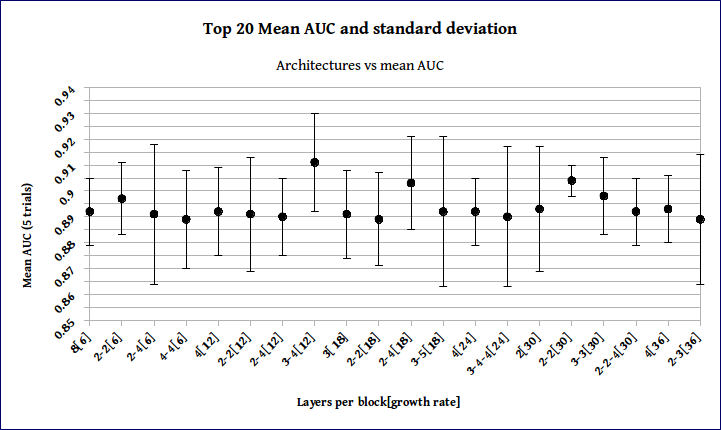
\includegraphics[width=0.5\textwidth]{images/densenet/auc_analysis_sortedby_growth.png}
%\caption{\label{fig:meanAUC_growth}AUC analysis sorted by number of growth rate.}
%\end{figure}

\begin{center}
 \begin{figure}[ht]
 \centering
 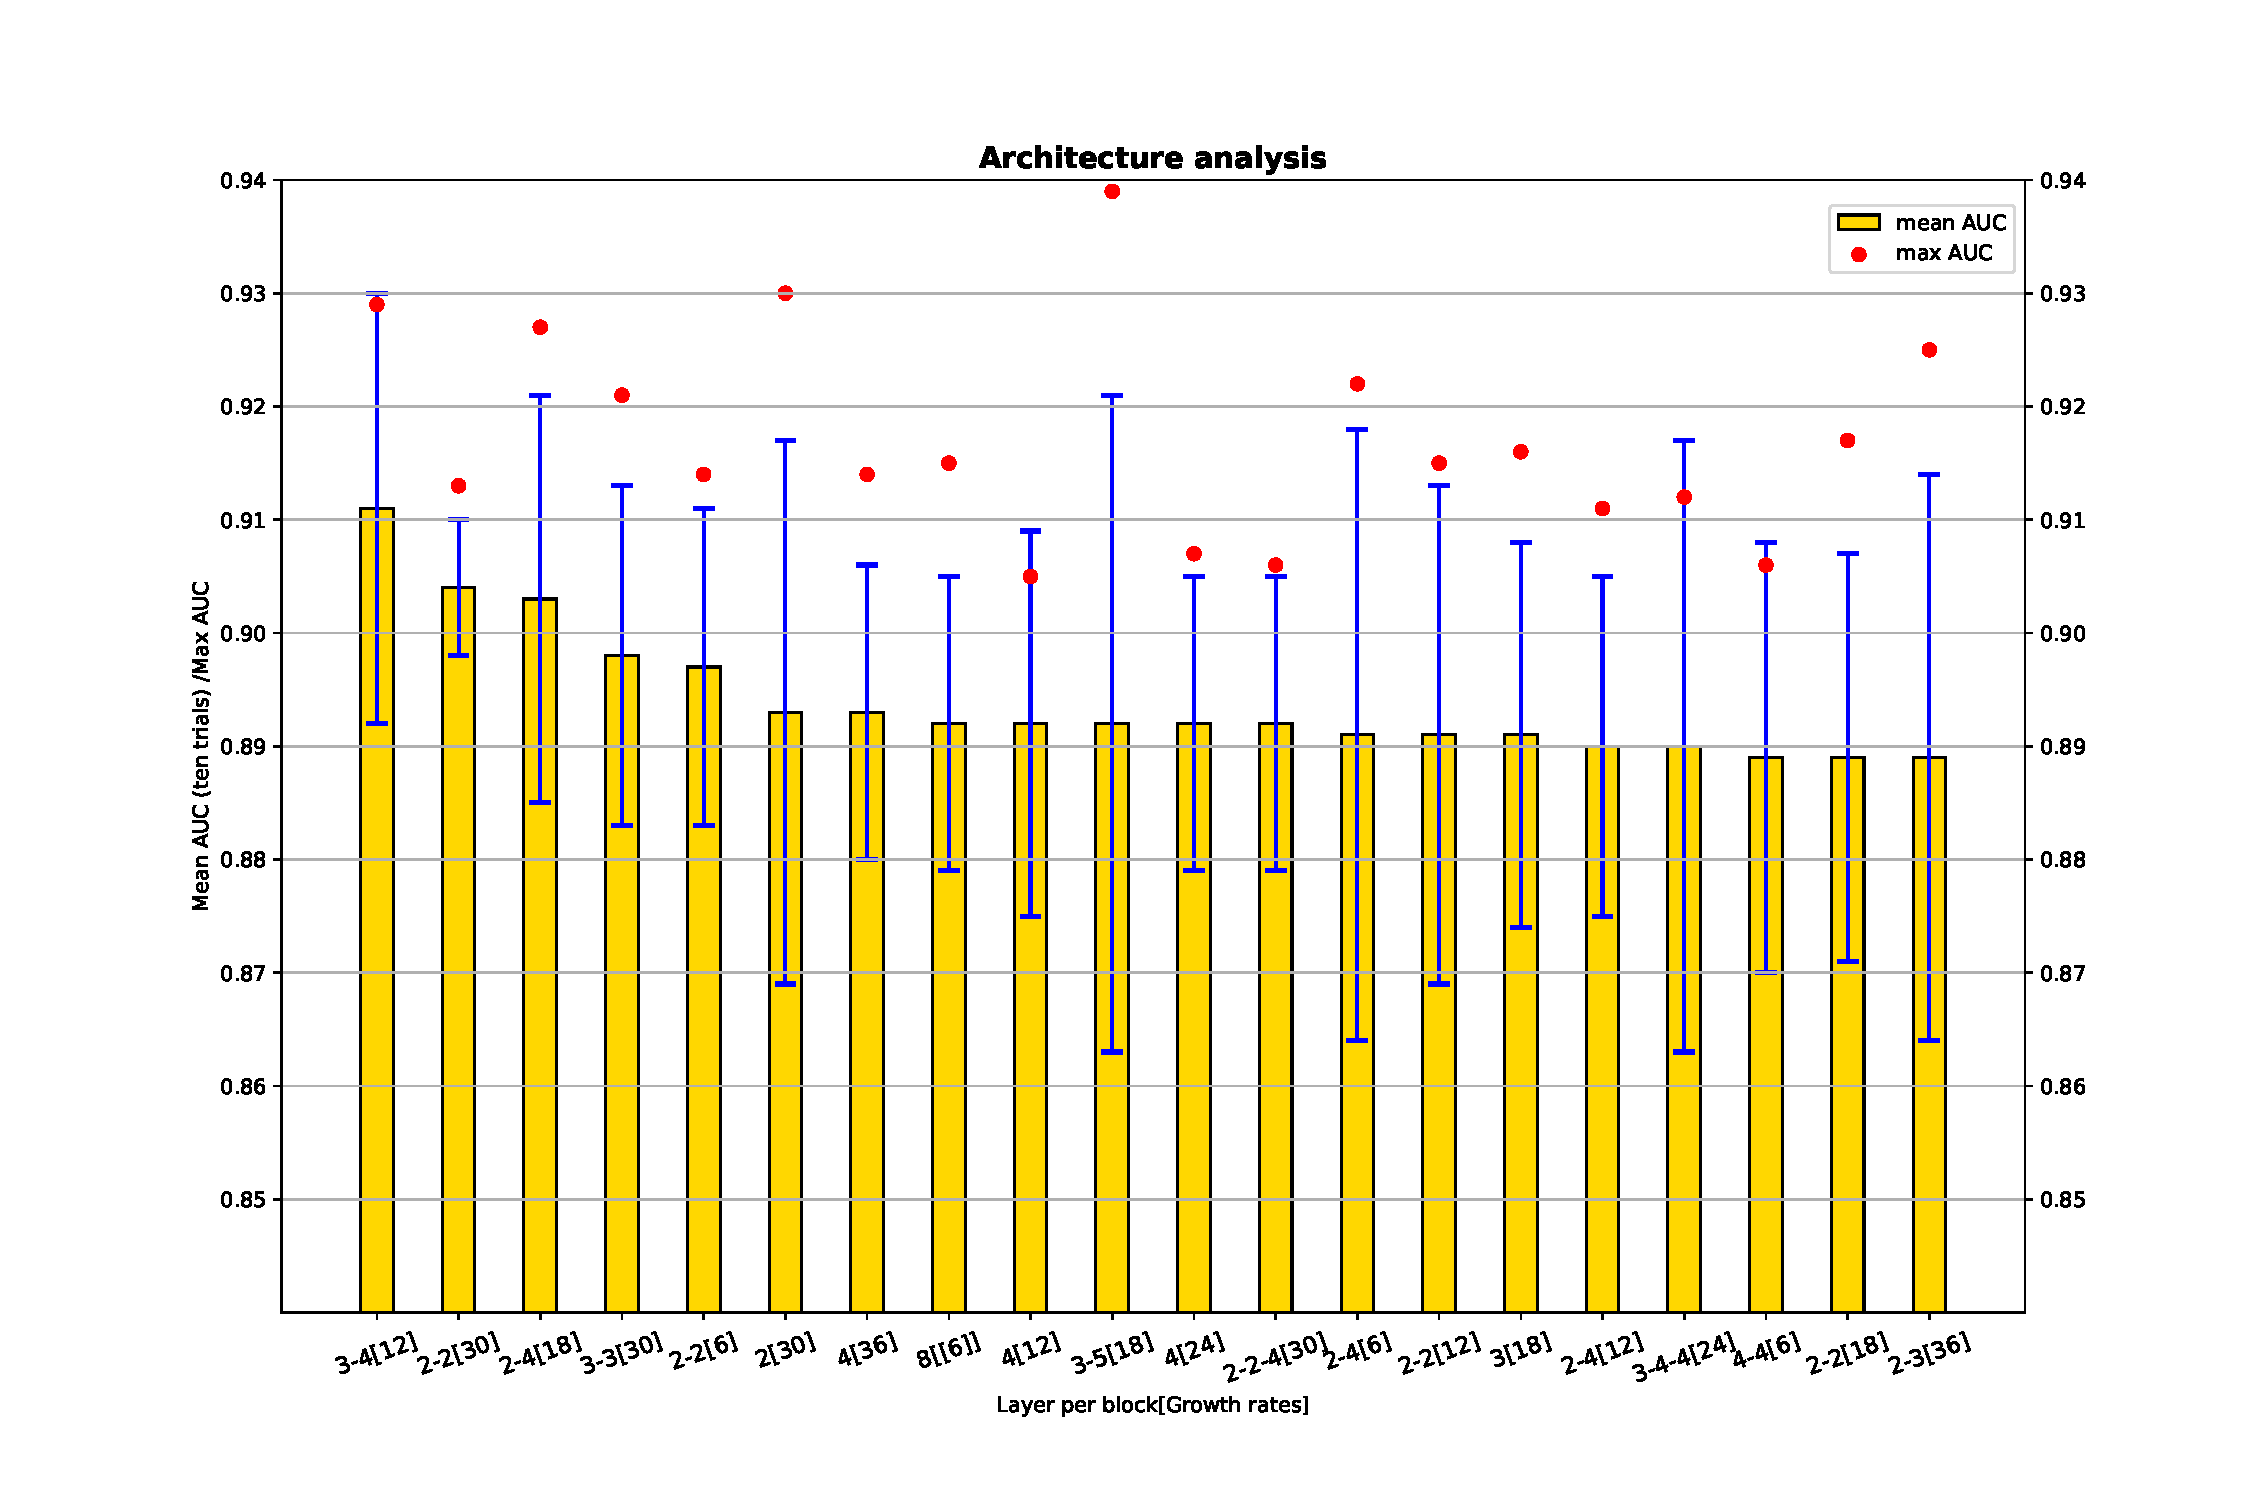
\includegraphics[width=16cm]{images/densenet/siamese/densenet_siamese_architecture_bar}
 \caption[DenseNet layers per block and growth rate mean AUC analysis]{DenseNet layers per block and growth rate analysis, sorted by mean AUC, high to low. In x-axis the layers per block and growth rate are displayed together, 
 with growth rate in brackets. It is easy to point out that, the top 20 is 
 dominated by the two layers architectures. The four layer ones do not come close at all. Just few three layer and some single layer architectures are showing good results.}
 \label{fig:meanAUC_growth_and_layers}
 \end{figure}
\end{center}

\paragraph{Discussion\\}
From figure \ref{fig:meanAUC_growth_and_layers} it is observed that the DenseNet with two dense blocks or layers (e.g., 2-2, 3-4) works best, ahead of single layer ones. Performance of the three and four layer DenseNets are not 
good. This is unexpected. According to the original paper \cite{densenet} the performance of a normal DenseNet increases as more deeper the network gets. However, in the original work the DenseNet is used individually as the 
feature extraction and decision network both. In this case, DenseNet is only used as the feature extraction network. Authors of \cite{densenet} though hinted that the depth of the network depends on the data volume available too.
For example for ImageNet \cite{imagenet}, authors used four layer DenseNet with high growth rates. But they used three layer DenseNet in other cases mostly. In any case when the DenseNet two-channel network is evaluated this issue can be 
verified with more conviction than with DenseNet-Siamese, simply because the DenseNet has been used in different way in this case. From figure \ref{fig:meanAUC_growth_and_layers} no strong trend for growth rate is observed, so 
further analysis or some other view of the data needs to be looked into. 
The network is evaluated 5 times for each configurations because it is observed that not every time the network performs exactly same way. Some times
it score much higher and some times it might even get stuck in a local minima. The weights of the network are randomly initiated using default initializer Glorot uniform \cite{kerasinit}. However many parameters are involved 
and because every time the weights are drawn randomly and the network gets trained from scratch, the decision boundary at the end of same number of epochs may look very different. Since there are too many networks to be evaluated
only 5 times each of them are evaluated, with the idea that the networks with good performance can be evaluated again for higher number of times to verify their consistency. 

\subsubsection{Performance Comparison Based On Maximum AUC}

There are some networks, specially three layer ones, which has comparatively poorer mean AUC but at least one of the 5 runs they has scored very high AUC. That is why all the architectures are sorted according to their maximum AUC in one
of the 5 trials. Displaying below in figure \ref{fig:maxAUC_five} is the \textbf{top 20} architectures (layers per dense block and growth rates) in terms of highest AUC on test data across 5 trials.

\begin{figure}[ht]
\centering
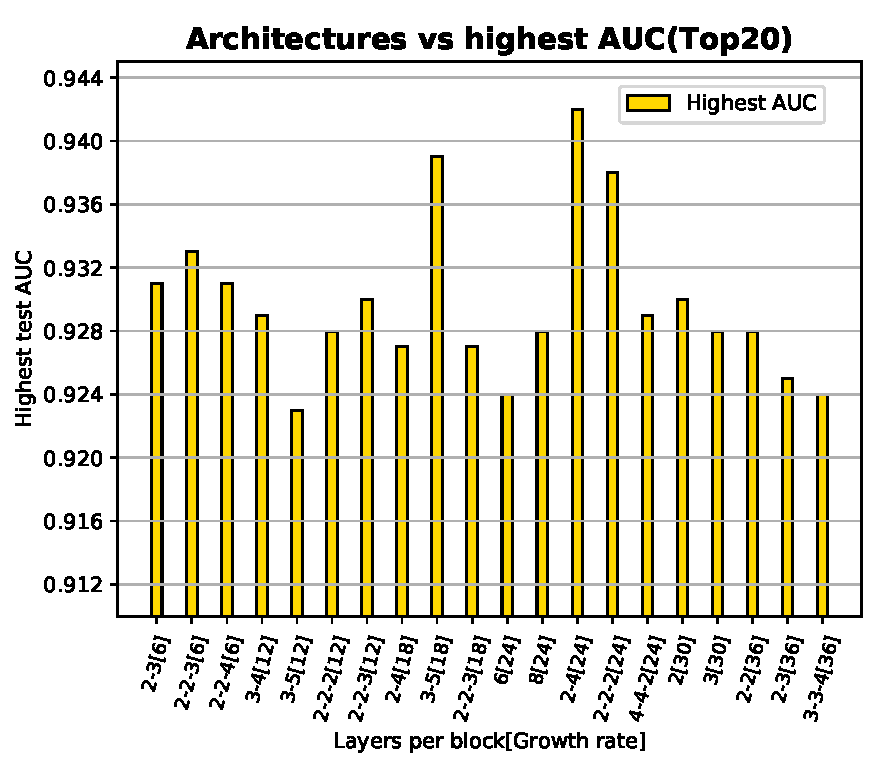
\includegraphics[width=0.8\textwidth]{images/densenet/siamese/densenet_siamese_max_bar}
\caption[DenseNet layers per block and growth rate max AUC analysis]{DenseNet layers per block and growth rate analysis, top 20 maximum AUC, sorted by growth rate. It seems the architectures growth rate 24 is most frequent here ahead of 12 and 18. unlike the top 20 mean AUC analysis many three layer
architectures are in this list.}
\label{fig:maxAUC_five}
\end{figure}

%\flushbottom
%\newpage 
\paragraph{Discussion\\}
 In both top 20 lists mentioned above the four dense block architectures did not make it in any of the case. Their performance on the test data is worse, so under current setup and assumptions they work worse than lesser block networks.
 Even though four layer networks are able to train above 95\% train accuracy their generalization on the test data seems to be poor in general.
 Two dense block networks in general works best in terms of mean AUC of the 5 evaluations.
 In terms of max AUC score some of the Three block and one block DenseNet works very good as well, but may not be that consistent in general and did not make it in the top 20 mean AUC list.
 Some networks though, like 2-2, 2-4, 3-4, 3-5, 3, 8, 2-2-4 etc are of special interest since they have featured in both the list of mean and max top 20 AUC. Even though the top 20 maximum AUC list is dominated by architectures with growth rate 
 24, in top 20 architectures based on mean AUC that is not the case. So still unable to select the best growth rate for the further evaluation. Hence further analysis is done for the best growth rate on a different view of the data.

\subsubsection{Optimal Growth Rate Analysis}
It is also important to find out the best growth rate for each of the architectures (layers per block). In the previous test each architectures are evaluated for growth rates: 6, 12, 18, 24, 30 and 36. 
For each architectures the growth rate for which the best mean AUC and best maximum AUC is recorded are displayed in the graph below (figure \ref{fig:best_growthrate})

\begin{figure}[ht]
\centering
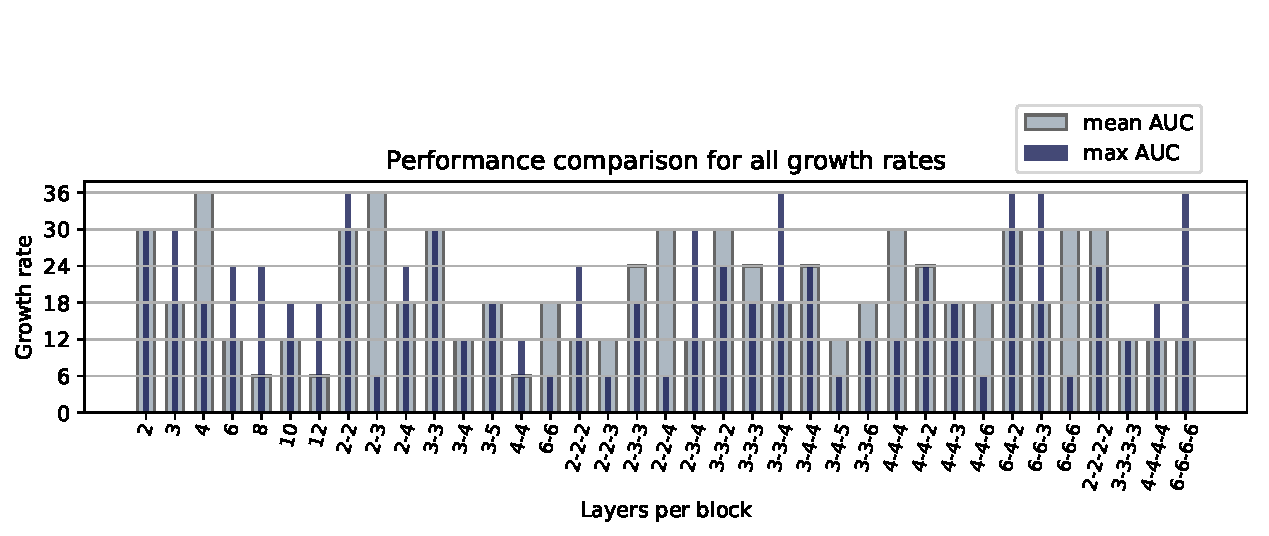
\includegraphics[width=1\textwidth]{images/densenet/siamese/densenet_siamese_gr_all_bar}
\caption[Best growth rate analysis.]{Best growth rate for each architectures are displayed based on mean AUC and max AUC. The grey column represents which growth rate ranked highest in mean AUC for the architecture, 
and the dark blue bar represents the growth rate for which the maximum AUC is recorded.}
\label{fig:best_growthrate}
\end{figure}

From figure \ref{fig:best_growthrate} it is observed that the growth rate for which each architecture have best mean and for which it has maximum AUC, might not always be same. For this purpose, histogram of 
best performing growth rates obtained from mean and max AUC analysis is displayed in the figure \ref{fig:growthrate_histogram} below:

\begin{figure}
  \centering
  \begin{subfigure}[b]{0.4\textwidth}
    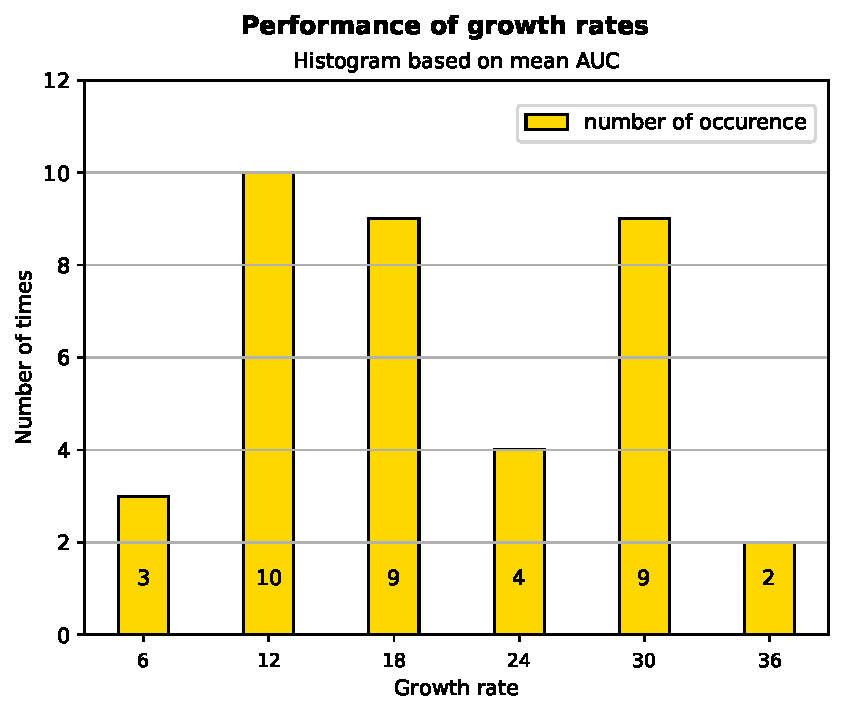
\includegraphics[width=\textwidth]{images/densenet/siamese/densenet_siamese_gr_mean_bar}
    \caption{Histogram of growth rates depending on mean AUC}
    \label{fig:mean_auc_histogram}
  \end{subfigure}
  ~ %add desired spacing between images, e. g. ~, \quad, \qquad, \hfill etc. 
   %(or a blank line to force the subfigure onto a new line)
  \begin{subfigure}[b]{0.4\textwidth}
    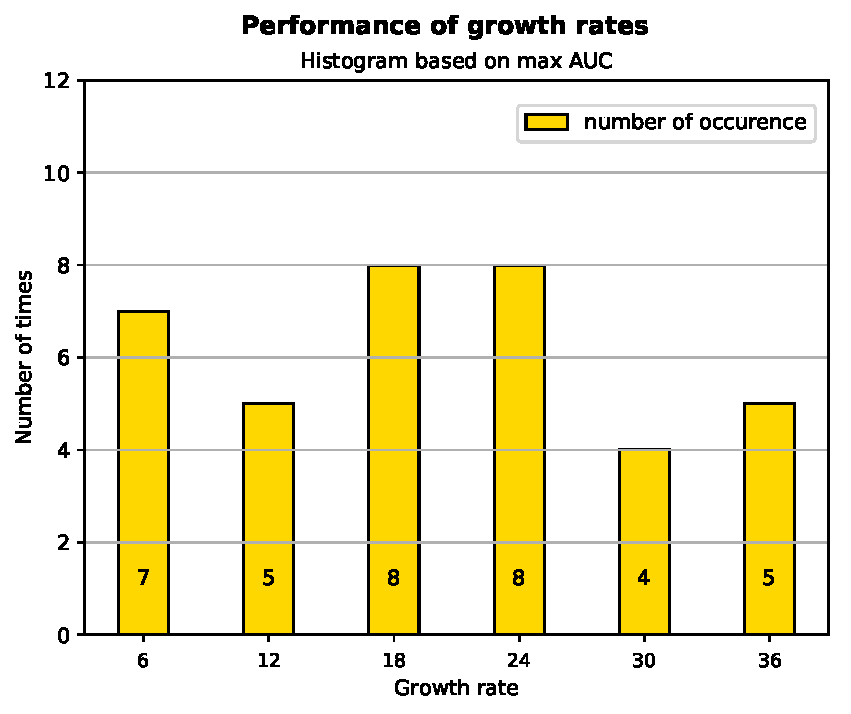
\includegraphics[width=\textwidth]{images/densenet/siamese/densenet_siamese_gr_max_bar}
    \caption{Histogram of growth rates depending on max AUC}
    \label{fig:max_auc_histogram}
  \end{subfigure}  
  \caption[Cumulative growth rate analysis (histograms)]{Cumulative growth rate analysis (histograms) }
  \label{fig:growthrate_histogram}
\end{figure}

\paragraph{Discussion\\}
It is evident from figure \ref{fig:max_auc_histogram}, based on the max AUC, there is no strong trend, its very random and inconclusive. Which is not very surprising given its just one run. 
With so many parameters and initialization and random dropouts involved, the network weights might learn very differently in spite of being trained in a same condition, resulting in a very different decision boundary.
In figure \ref{fig:mean_auc_histogram} it is visible that the contribution of growth rate 6 and growth rate 36 is really less, so probably they are too thin or too thick for the data. 
From figure \ref{fig:growthrate_histogram} above it is safe to assume that growth rate 18 is very good performer in both analysis. Which also makes sense since it is neither too thin nor too thick. Because this conclusion 
is based on just 5 evaluations of each architectures, it make sense to experiment with other growth rates(except 6,36) as well for finer evaluation.

\flushbottom
\newpage
\subsection{Total Parameters Analysis}
It might be surprising but the single dense block networks have \textbf{most} parameters. This is because of the flatten pooling that is used here in this work instead of global average pooling 2D. 
%A example output can be compared between 2 and 2-2 for same growth rate
And four block networks have the least total and trainable parameters. %This is also supported by the theory in the paper \cite{densenet} the more layers the network has the number of parameters gets lesser.
How ever as the number of dense blocks keeps getting higher the non-trainable parameters also gets higher. So 4 blocks dense net has most number of non-trainable parameters.
For the visualization of the comparison 2, 2-2, 2-2-2, 2-2-2-2 layers per block DenseNet's parameter sizes are compared below, all recorded for growth rate 18.

\begin{figure}[ht]
  \centering
  \begin{subfigure}[b]{0.4\textwidth}
    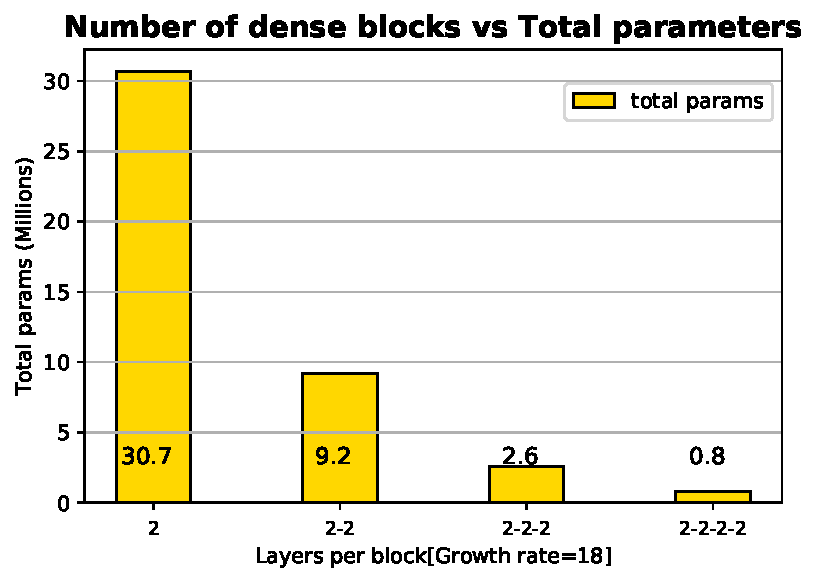
\includegraphics[height=4cm]{images/densenet/siamese/densenet_siamese_blocks_params_bar}
    \caption{Parameters vs architectures}
    \label{fig:Denseblocks_vs_parameters}
  \end{subfigure}
  ~ %add desired spacing between images, e. g. ~, \quad, \qquad, \hfill etc. 
   %(or a blank line to force the subfigure onto a new line)
  \begin{subfigure}[b]{0.4\textwidth}
    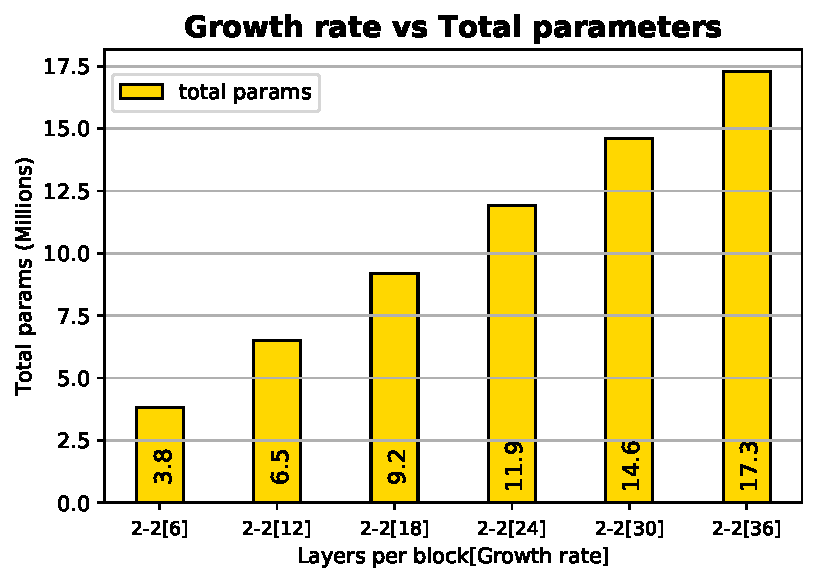
\includegraphics[height=4cm]{images/densenet/siamese/densenet_siamese_gr_params_bar}
    \caption{Parameters vs growth rates}
    \label{fig:growthrate_vs_parameters}
  \end{subfigure}  
  \caption{Total number of parameters analysis}
  \label{fig:total_parameters_densenet}
\end{figure}

In figure \ref{fig:growthrate_vs_parameters} it is shown that with growth rate increase the total parameter size also increases. For this purpose the parameters for all the growth rates compared for architecture 2-2.

\subsection{Standard Deviation Across Blocks}
Another trend is observed that the standard deviation varies more as the number of dense blocks increase. 
So the standard deviation values for all the readings are collected for 1, 2, 3, 4 number of dense blocks (nb\_dense\_blocks) separately and their average values are presented in the table below.

\begin{figure}[ht]
\centering
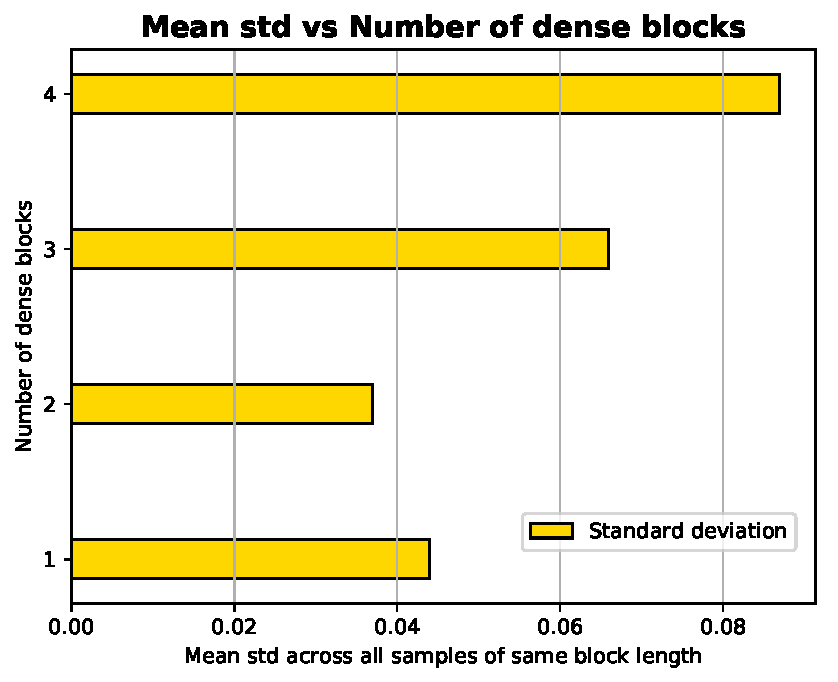
\includegraphics[width=6cm]{images/densenet/siamese/densenet_siamese_std_blocks_bar}
\label{std_dense_blocks}
\caption{Average standard deviation on AUC across networks with same number of dense blocks, e.g., 2-2 and 3-3 has 2 dense blocks, 2-2-2, 3-4-5 has 3 dense blocks etc.}
\end{figure}

Even though the number of sample size differs a lot, 42, 48, 108, 24 samples for dense blocks 1, 2, 3, 4 respectively, it is observed that standard deviation of AUC is higher for dense block 3 and 4.
It is probably because the blocks 3 and 4 networks have much lesser parameters than the 1 and 2 number of dense blocks. It is clear from this analysis that the two layer architecture is the best.\\

At this point, the best possible values of the growth rate and layers per block have been obtained. But the search space for the architectures are still big and needs to shortened further and basically chose up to 3 networks so that further 
evaluations can be done. 

\subsection{Finer Grid Search Analysis}
From the first analysis the top 5 network based on mean AUC of 5 trials (figure \ref{fig:meanAUC_growth_and_layers}) and top 5 network obtaining maximum AUC (figure \ref{fig:maxAUC_five}) are further evaluated for \textbf{20} 
evaluations each, after training from scratch. This 10 architectures will be referred as top 10 architectures in following analysis. All other test conditions remain the same. Results after 20 times evaluation is expected to 
be more dependable than 5 trials. In the chart \ref{fig:arch_vs_auc_finer} the mean AUC of 20 evaluations and it's standard deviation is displayed in yellow bars and blue lines respectively. 
While in red displayed the maximum AUC obtained in 20 evaluations.

\begin{figure}[ht]
\centering
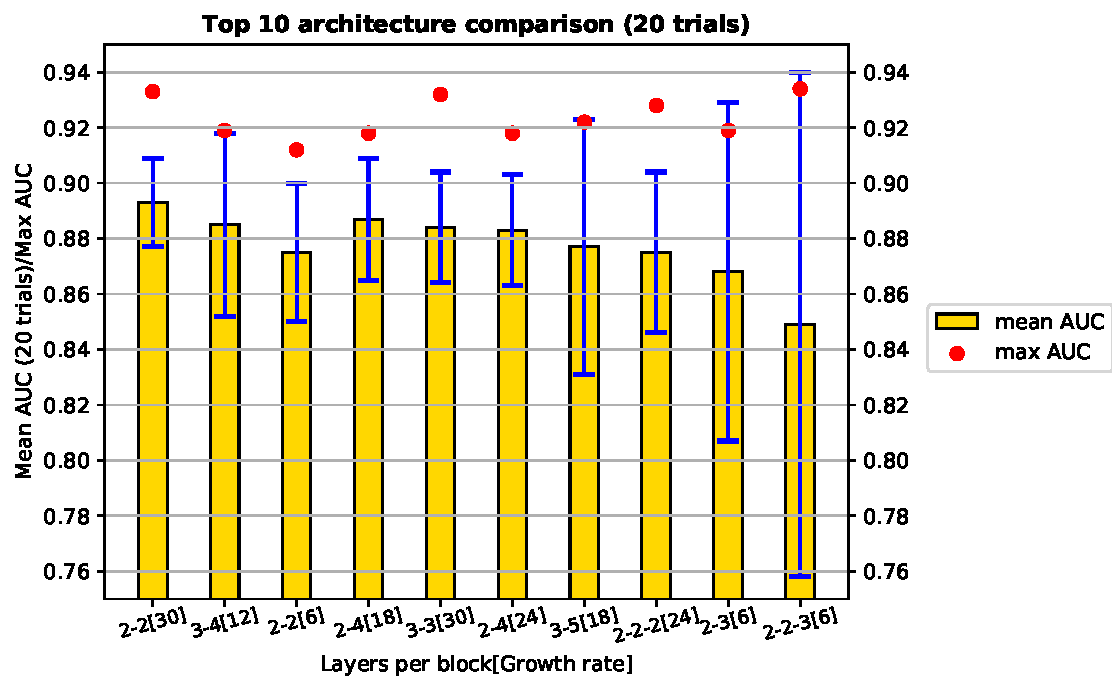
\includegraphics[width=13cm,height=7cm]{images/densenet/siamese/densenet_siamese_finer_search}
\caption{Finer search with top 10 architectures}
\label{fig:arch_vs_auc_finer}
\end{figure}

Same data is displayed in table \ref{table:arch_vs_auc_finer_table} but in decreasing order of the best mean AUC.

\begin{table}[ht]
\centering
\caption[Finer search with 10 architectures]{Finer search results for 20 evaluation of previous top 10 architectures. Sorted according to mean AUC.}
 \begin{tabular}{|c c c c c|} 
 \hline\hline
 \rowcolor{lightgrey}
 Layers & Growth rate & Mean AUC & Std & Max AUC\\
 2-2 & 30 & 0.893 & 0.016 & 0.933\\
 3-4 & 12 & 0.885 & 0.033 & 0.919\\
 2-2 & 6 & 0.875 & 0.025 & 0.912\\
 2-4 & 18 & 0.887 & 0.022 & 0.918\\
 3-3 & 30 & 0.884 & 0.02 & 0.932\\
 2-4 & 24 & 0.883 & 0.02 & 0.918\\
 3-5 & 18 & 0.877 & 0.046 & 0.922\\
 2-2-2 & 24 & 0.875 & 0.029 & 0.928\\
 2-3 & 6 & 0.868 & 0.061 & 0.919\\
 2-2-3 & 6 & 0.849 & 0.091 & 0.934\\
 \hline \hline
\end{tabular}
\label{table:arch_vs_auc_finer_table}
\end{table}

\newpage
\paragraph{Discussion\\}
It is observed that in 20 evaluations layers 2-2 with growth rate 30 is the best result both in terms of lowest standard of deviation and highest mean AUC. As it happens its also second highest in terms of the 
 maximum AUC 0.933 just behind 0.934 from 2-2-3.
3-4, 2-4 networks are also performing well in terms of mean AUC. Their results are very close as well, so just evaluating 3-4 network for the finer analysis.
2-2-3 layers is interesting though, it has the highest standard deviation but 2 or 3 very good AUC scores too. So it needs to be further looked into.

\begin{figure}[htp]
\centering
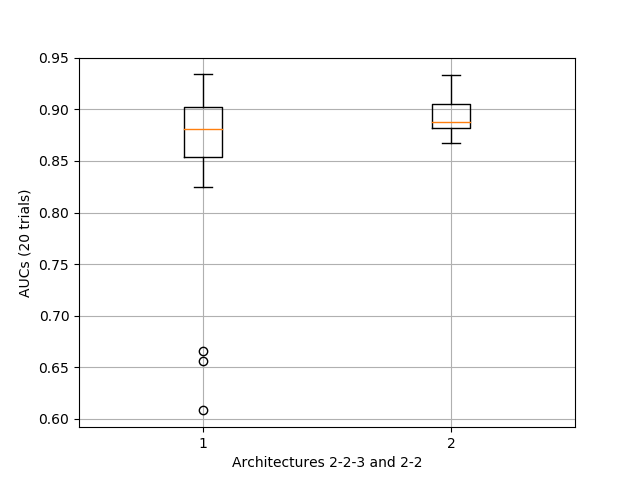
\includegraphics[width=9cm]{images/densenet/arch_compare_boxplot.png}
\caption{Box and whisker plot representation of AUC predictions of 2-2-3 and 2-2 architectures. First boxplot is for 2-2-3.}
\label{fig:arch_compare_boxplot}
\end{figure}

In figure \ref{fig:arch_compare_boxplot} the five number summary(min, first quartile Q1, median, third quartile Q3, max) is compared for architecture 2-2 and 2-2-3. For architecture 2-2-3, 3 AUC readings are detected as outliers 
out of 20 trials at 0.666, 0.608, 0.656 AUC. The outliers are affecting the overall mean auc for 2-2-3 network, also causing big standard deviation. This outliers are probably caused by training getting stuck in local minima or similar. 
2-2 is found to be more consistent, it has no outliers. It is believed that consistency is desirable for a network. Hence 2-2-3 network is ruled out of contention for the best network, because of it's lack of consistency.
though the overall concept of terming few prediction accuracies as outlier can be debatable. It is the nature of the network. At least, it is clear that three prediction accuracies are way of than other 17 predictions.

%TODO should they go to the appendix
\paragraph{Five Number Summary\\}
Also the brief introduction to the five number summary is as follows. \textbf{The minimum} is the smallest datum in the dataset. \textbf{The first quartile} is chosen so that 25\% data points are lesser than it, similarly \textbf{the median}
is the middle point (50\%) of the dataset, and \textbf{the third quartile} is the point where 75\% data falls below it. Lastly \textbf{the maximum} is simply the highest datum in the data set. All together this five criteria 
represents different aspects of any distribution.

\paragraph{Box And Whisker Plot Interpretation\\}
Box and whisker plot \cite{boxplot}, where the box represent the interquartile range between first quartile 25\% (Q1) and third quartile 75\% (Q3) for the data range, and the orange line is for the median and the extended whiskers display the 
range of the maximum and minimum data points in the distribution. The interquartile range denoted by IQR, is the difference between Q3 and Q1. Outliers are the data points that reside outside the stretch of [(Q1-1.5*IQR), (Q3+1.5*IQR)].
The fraction 1.5 here is the default value in 'matplotlib' and also used in this work for all the evaluations. So if the data points lie outside the aforementioned range, then those are displayed as little dots or hollow circles in the plot 
beyond the whiskers.


\subsection{Number Of Filter Analysis}
Initial number of filter (parameter name 'nb\_filter') values 8, 16, 32, 64 are being evaluated here. Also a comparison between mean prediction AUCs obtained for growth rate 18 and 30 is done under this analysis. Ten evaluations of each test cases has been done.

\begin{figure}[ht]
\centering
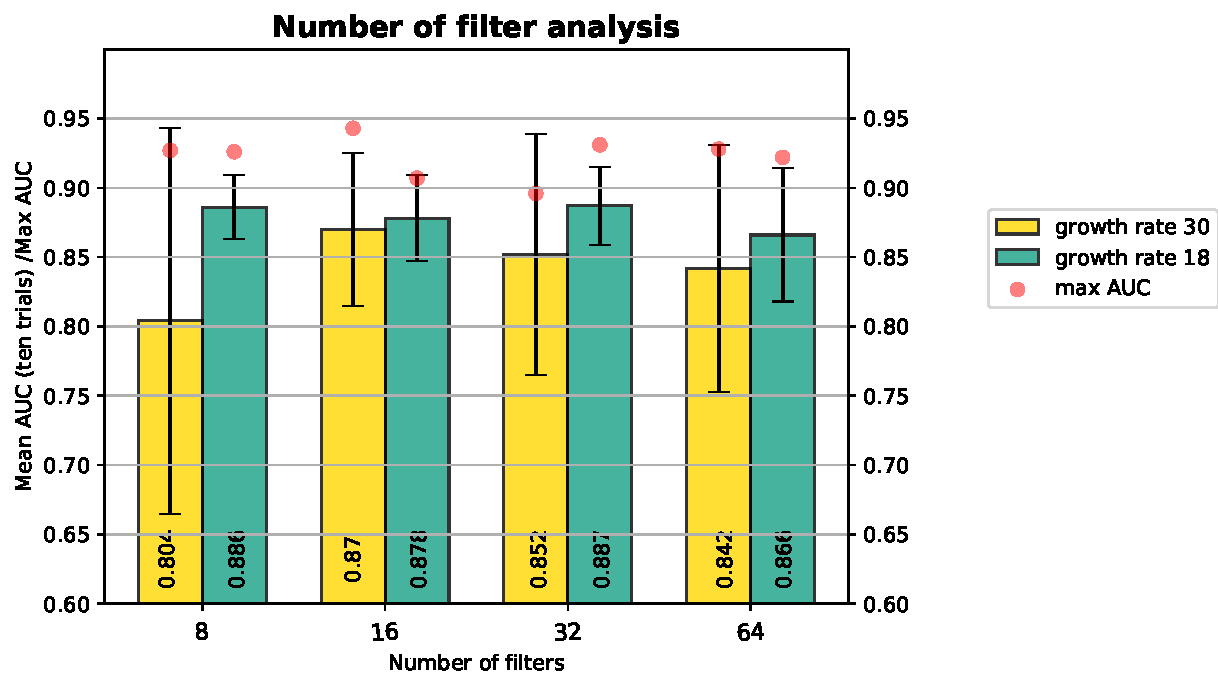
\includegraphics[width = 12cm, height=6cm]{images/densenet/siamese/densenet_siamese_nb_filter}
\caption{Number of filter analysis for different growth rates}
\label{fig:nb_filter_vs_auc_growthrate_compare}
\end{figure}

\paragraph{Discussion\\}
figure \ref{fig:nb_filter_vs_auc_growthrate_compare} shows that the number of filter 16 works better than others for growth rate 30 and also happen to have the Maximum AUC recorded and lowest standard deviation as well. 
It seems for thinner networks (lower growth rates), change in number of filter value matters lesser than the thicker networks. 
Since for 18 growth rate the mean AUC for all the values of 'nb\_filter' are very close. But there is lot of difference for growth rate 30 for different rates.
However both the networks are found to work pretty good with number of filter value of 16. This could have been further evaluated with more growth rates, but for this work it is concluded with 16 as our best nb\_filter value.

\subsection{DenseNet Dropout Probability Analysis}
As usual ten evaluations done for each dropout probabilities displayed in figure \ref{fig:auc_vs_densenet_dropout}. Mean AUC is best for dropout 0.4. Maximum AUC is highest for dropout 0.5.
Now it is no surprise that with 0, 0.1 and 0.7 dropouts the results are not the best, because it's either too less or too much regularization. But it is bit unexpected to have dropout probability 0.3 and 0.5 performing low. 
probabilities 0.2, 0.4 are chosen as the best dropout rate values for future evaluations because they have comparatively better max AUC and mean AUC.

\begin{figure}[ht]
\centering
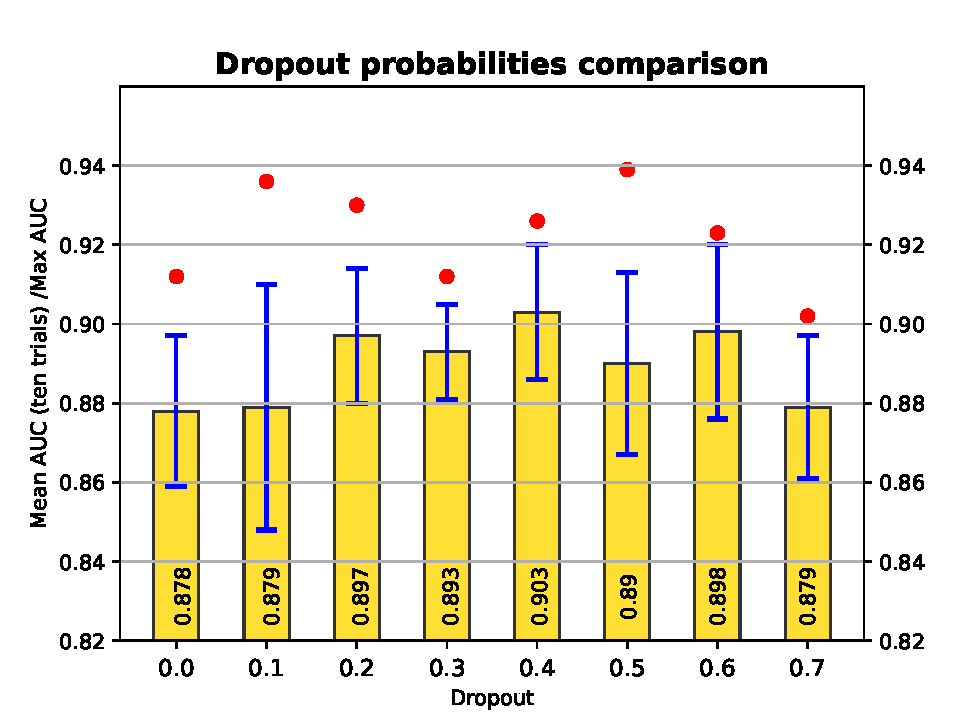
\includegraphics[width=9cm,height=6cm]{images/densenet/siamese/densenet_siamese_dropout}
\caption{DenseNet dropout probability analysis.}
\label{fig:auc_vs_densenet_dropout}
\end{figure}

%\paragraph{Discussion\\}

\subsection{Reduction And Bottleneck Analysis}
The evaluation results for the bottleneck and reduction are displayed in the figure \ref{fig:compression_and_bottleneck_vs_auc}.

\begin{figure}[ht]
\centering
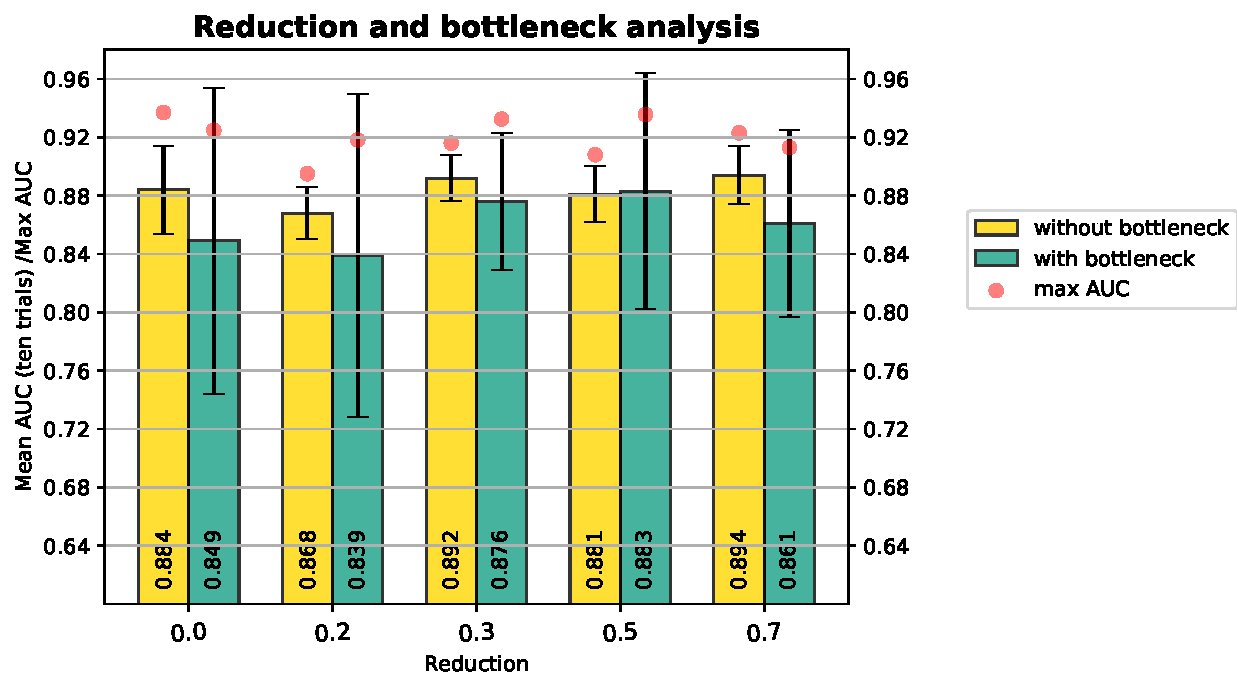
\includegraphics[width=12cm,height=5cm]{images/densenet/siamese/densenet_siamese_reduction_bottleneck}
\caption{Evaluation of reduction and bottleneck and mean AUC(across 10 trials). The max AUC obtained by one of the trial is also displayed separately for experiment with bottleneck and without bottleneck.}
\label{fig:compression_and_bottleneck_vs_auc}
\end{figure}

\begin{figure}[ht]
\centering
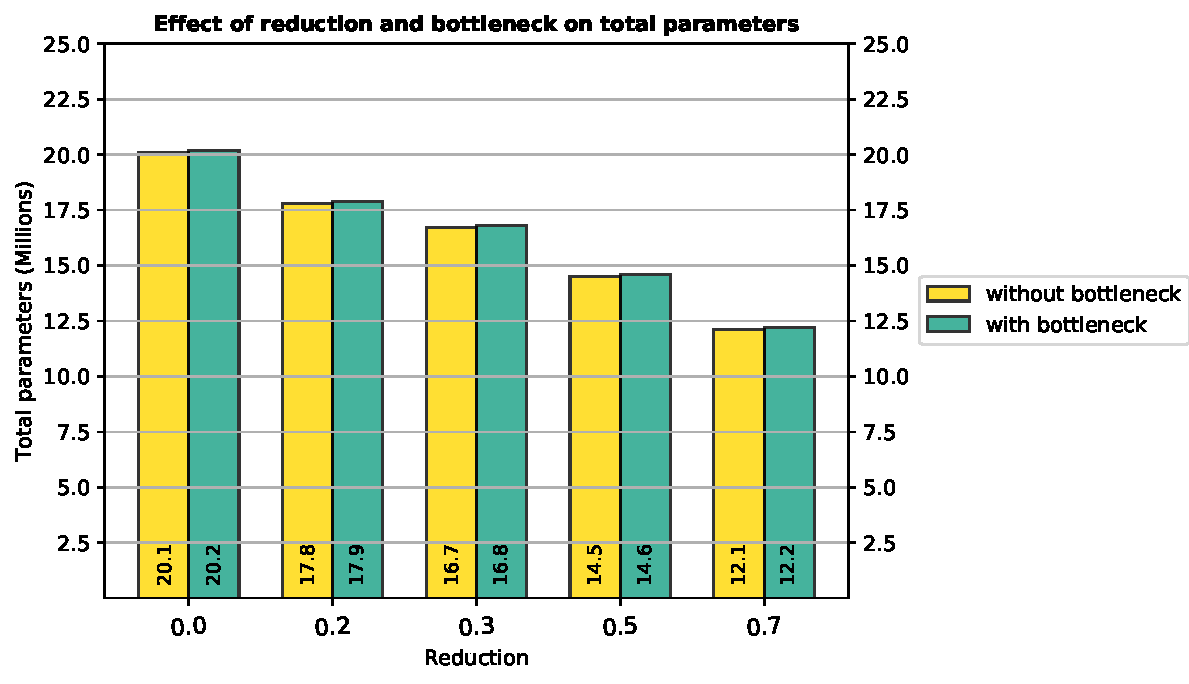
\includegraphics[width=12cm,height=5cm]{images/densenet/siamese/densenet_siamese_params_reduction_bottleneck}
\caption{The total parameters are varying with reduction. It also gets affected by use of bottleneck, how ever that is very minimal.}
\label{fig:compression_and_bn_vs_parameters}
\end{figure}

\paragraph{Discussion\\}
The use of reduction really makes the model much more compact without losing the effectiveness. From figure \ref{fig:compression_and_bn_vs_parameters} it is observed that without reduction the parameter size is 20.1 Millions, 
after using reduction of 0.7 the mean AUC is still as good but the total parameter size has become 12.1 millions. Use of bottleneck does in-fact increase the parameters by little more than 0.1 million, but it does not improve the 
results at all. So this is a unexpected behavior. Bottleneck also has much higher standard deviation. Theoretically it is suppose to help making the model more compact. But over all effect on the data is observed to be adverse.
But the max auc values still belong to the bottleneck layers 3 out of 5 times. Other two times also its close to highest. That's perhaps interesting to note. So the best reduction ratio chosen, based on the mean AUC are 0.7 and 0.3.
Bottleneck will not be enabled for further evaluations.

\subsection{Fully Connected Layer Dropout Analysis}
In the diagram \ref{fig:siamese_densenet_structure_wraped} the hyperparameters associated to the decision network part are displayed. 

\begin{wrapfigure}[12]{r}{6cm}
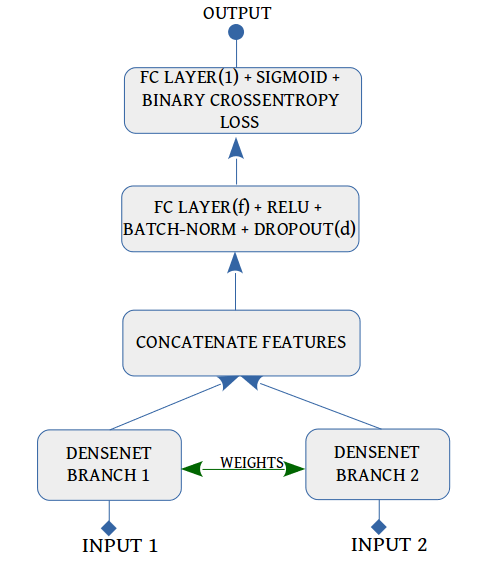
\includegraphics[width=5cm]{images/densenet/siamese_densenet_structure}
\caption{Hyperparameters in DenseNet-Siamese architecture}
\label{fig:siamese_densenet_structure_wraped}
\end{wrapfigure} 

The dropout probability connected to the first FC layer of the Siamese part is evaluated here, shown as d in \ref{fig:siamese_densenet_structure_wraped}. The search space evaluated for the d is as follows: [0, 0.1, 0.2, 0.3, 0.4, 0.5, 0.6, 0.7].

\paragraph{Discussion\\}
From figure \ref{fig:fc_dropout} it can be observed that for dropout probability 0.5 the network has the highest mean AUC along with dropout probability 0.7. 
The mean AUCs for 0.3, 0.4 is lower than expected and for 0.7 is much higher. The best values for dropout probability chosen for further evaluation are 0.5 and 0.7 both.\\
\begin{figure}[ht]
\centering
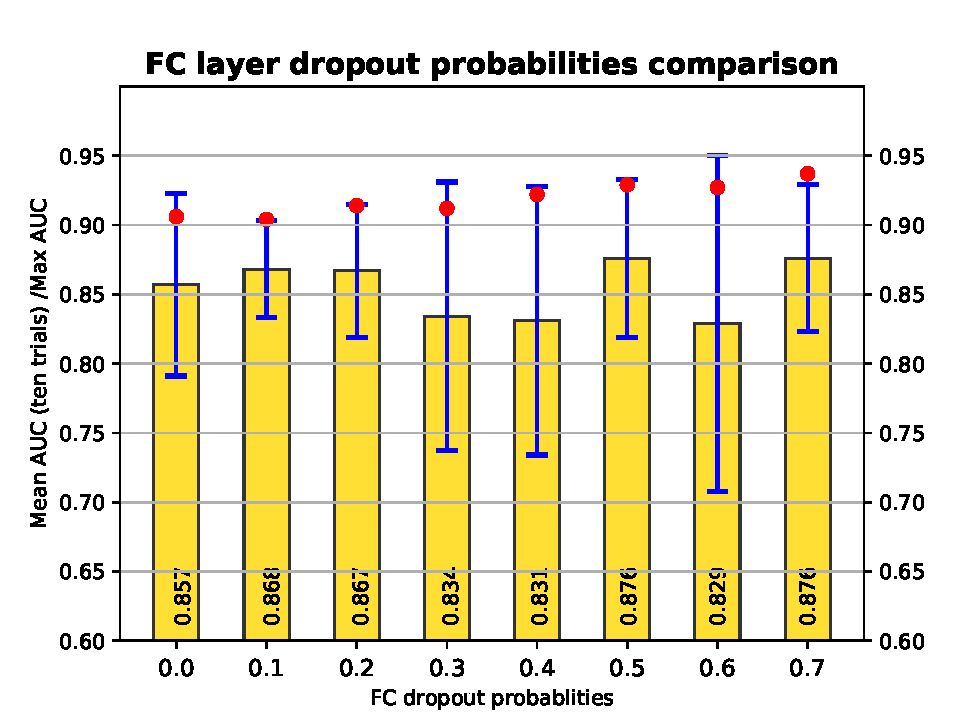
\includegraphics[width=12cm,height=6cm]{images/densenet/siamese/densenet_siamese_FC_dropout}
\caption{Optimal dropout (d) probabilities for FC layer analysis}
\label{fig:fc_dropout}
\end{figure}



\subsection{Fully Connected Layer Output Size Analysis}
The FC layer output size is denoted by f in figure \ref{fig:siamese_densenet_structure_wraped}.
The fully-connected layers are initialized (kernel) with “He normal” initialization.
\begin{figure}[ht]
\centering
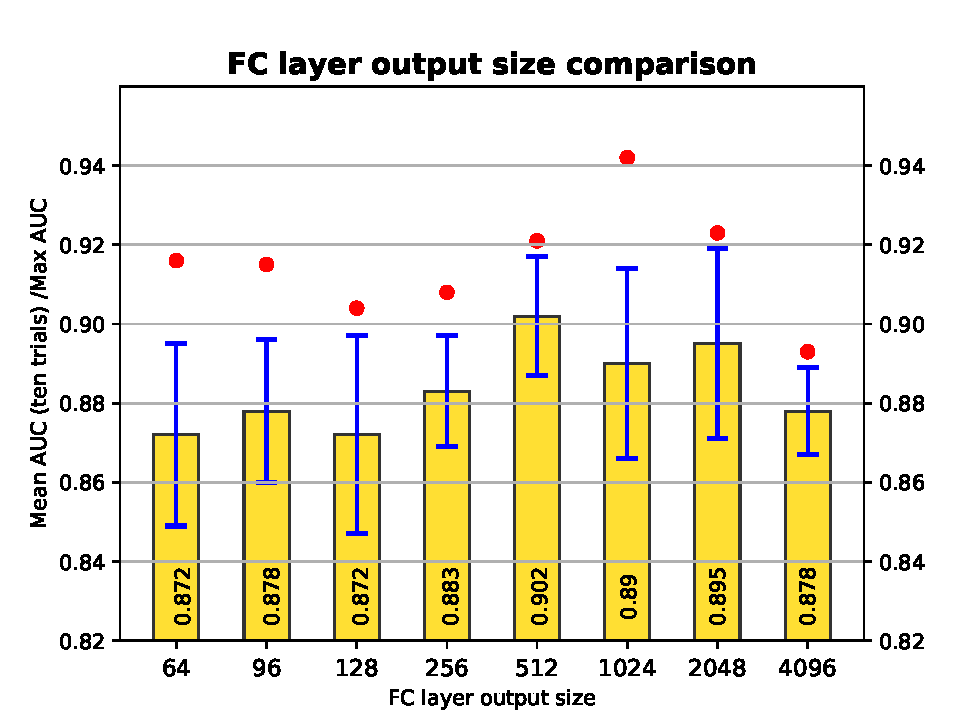
\includegraphics[width=9cm,height=5cm]{images/densenet/siamese/densenet_siamese_FC_out}
\caption{Optimal FC filter size (f) analysis.}
\label{fig:fc_filter_size}
\end{figure}

\paragraph{Discussion\\}
Whole search space is shown in figure \ref{fig:fc_filter_size}. The output (f) value 512 yielded the best mean AUC (from the figure \ref{fig:fc_filter_size} ). Though the max AUC obtained by the f=1024 and f=2048 is also scoring very good.
However on this value of f the number of total parameters for the whole network depends as the whole feature map of each DenseNet branch are flattened using “flatten” then concatenated.
Hence multiplied by 2 (since 2 branches). This concatenated feature map is then multiplied by the f size when they gets connected.
For example one DenseNet branch has feature map has size=n, concatenated feature map has size=2n. Concatenated features gets connected to FC network with output size f results in 2n*f parameters increase, and produces output size = f.
In other words the smallest f size which gives good performance, is better since it keeps the computations smaller. So f=512 is chosen.

\subsection{Batch Size Analysis}
If the batch size is too low then it takes more time and after a certain size it does not train well too.If the batch size is very big then it may train faster but they generalize lesser as they tend to converge to 
sharp minimizers of the training function \cite{keskar2016large}.

\begin{figure}[ht]
\centering
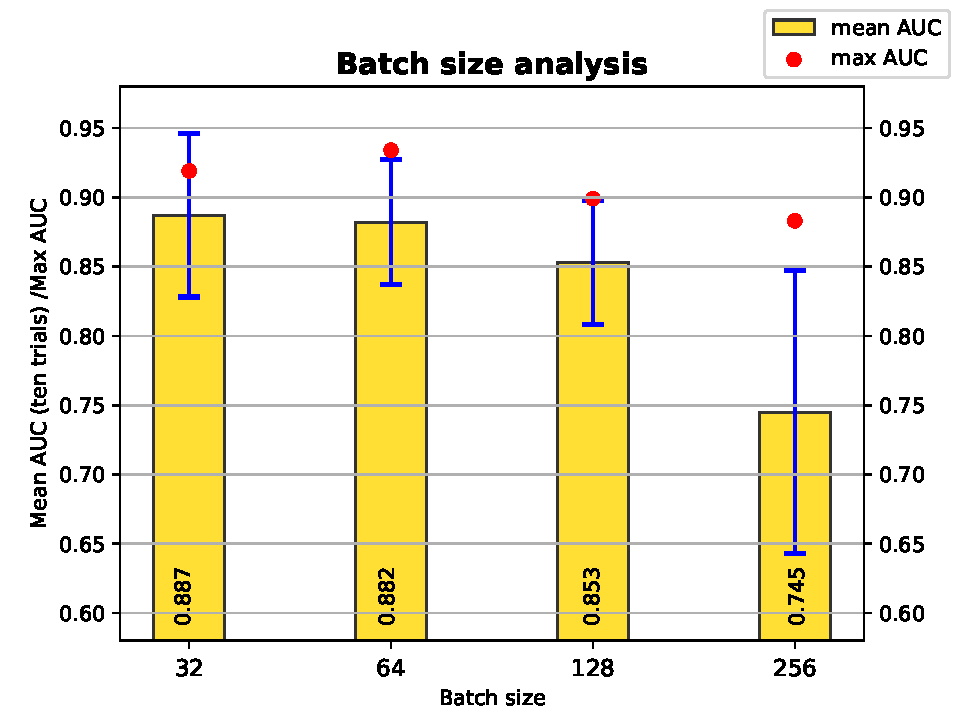
\includegraphics[width=7cm,height=4cm]{images/densenet/siamese/densenet_siamese_batchsize}
\caption{DenseNet-Siamese optimal batch size analysis.}
\label{fig:batch_size}
\end{figure}

\paragraph{Discussion\\}
From the figure \ref{fig:batch_size} it is observed that the larger the batch size gets the prediction accuracy on the test data gets worse. Mean prediction AUC for batch size 32 and 64 are very close.
The max AUC score for batch size 64 is much higher than 32 and it will train faster too, that is why it is selected as the best value. 

\subsection{Learning Rate And Optimizer Analysis}

During the training, in backpropagation step, the analytic gradient is computed which is used to update the parameters of the network (inspired by \cite{ruder}. This update stage could be done in different ways, 
this is where the optimizer come into action. While the main target of the deep learning task is to find the minima, the optimizers can control how soon or robustly the minima is found. There is a very compelling 
comparison of optimization process to a ball or particle rolling down hill in the Stanford lecture series \cite{cs231n}. It compares the loss function to a hill and randomly initializing the network weights to a particle with 
zero velocity at random points on the hill. Now the optimization process is compared to simulating the particle's motion (parameter vector) of rolling down the hill landscape (loss).

Keras sources \cite{kerasopt} gives very brief description of the optimizers. Important optimizers are as follows: \textbf{SGD} Stochastic gradient descent optimizer, the very first of it's kind, conceptualized by H. 
Robbins and S. Munro back in 1951. Even though it remains one of the most preferred optimizer till date 
(different variations available e.g., with momentum, Nesterov etc), this optimizer is not evaluated in this work in favor of more theoretically advanced optimizers. In \textbf{Adagrad} instead of globally varying the learning rate, 
the concept of per parameter adaptive learning rate is first introduced by Duchi et al. in Adagrad optimizer. It seems it has a limitation though, the use of monotonic learning rate is often too aggressive and the 
learning stops too early. This optimizer is also not included in this study in favor of more advanced optimizers. \textbf{RMSprop} try to compensate the aggressive monotonically decreasing learning rate from 
Adagrad by introducing the moving average of squared gradient. \textbf{Adam} can be seen as RMSprop with momentum. \textbf{Nadam} incorporates Nesterov momentum into Adam. \textbf{Adamax} is a variant 
of Adam which uses infinity norm. \textbf{Adadelta} is like Adagrad with moving window of gradient updates.\\

Optimal learning rate selection is very important for effective learning. However, optimal learning rate varies optimizer to optimizer, hence for learning rate and optimizer a very fine grained search is performed here
The search space contains total 20 different learning rates and five optimizers. Each optimizer is evaluated for all 20 learning rates, that makes 100 network configurations which are trained 10 times from scratch 
for the evaluation and compared on the prediction accuracy (AUC) and std as usual. The search space is presented in table \ref{table:search_space_optimizers}:

\begin{table}[ht]
 \centering
 \caption{The search space for learning rate and optimizer best hyperparameters. Since both are related they need to be evaluated together.}
 \begin{tabular}{|l|} 
 \hline\hline
 \rowcolor{lightgrey}
 Learning rate \\[0.5ex] 
 \hline
 0.1, 0.5, 1.0 (only for Adadelta)\\
 0.01, 0.02, 0.03, 0.05, 0.07\\
 0.001, 0.002, 0.003, 0.005, 0.007\\
 0.0001, 0.0002, 0.0003, 0.0005, 0.0007\\
 0.00001, 0.00002, 0.00003, 0.00005, 0.00007\\
 \rowcolor{lightgrey}
 \hline
 Optimizers\\
 \hline
 Adam, Nadam, Adamax, RMSprop, Adadelta \\
 \hline \hline
\end{tabular}
\label{table:search_space_optimizers}
\end{table}

The evaluation results are presented in figure \ref{fig:lr_optimizers} where the results for different learning rate are compared for each of the optimizers. In figure \ref{fig:lr_optimizers_compare} different representation of the evaluation
result is presented which offers the comparative view for each of the optimizers for specific learning rate.

\begin{figure}[ht]
\centering
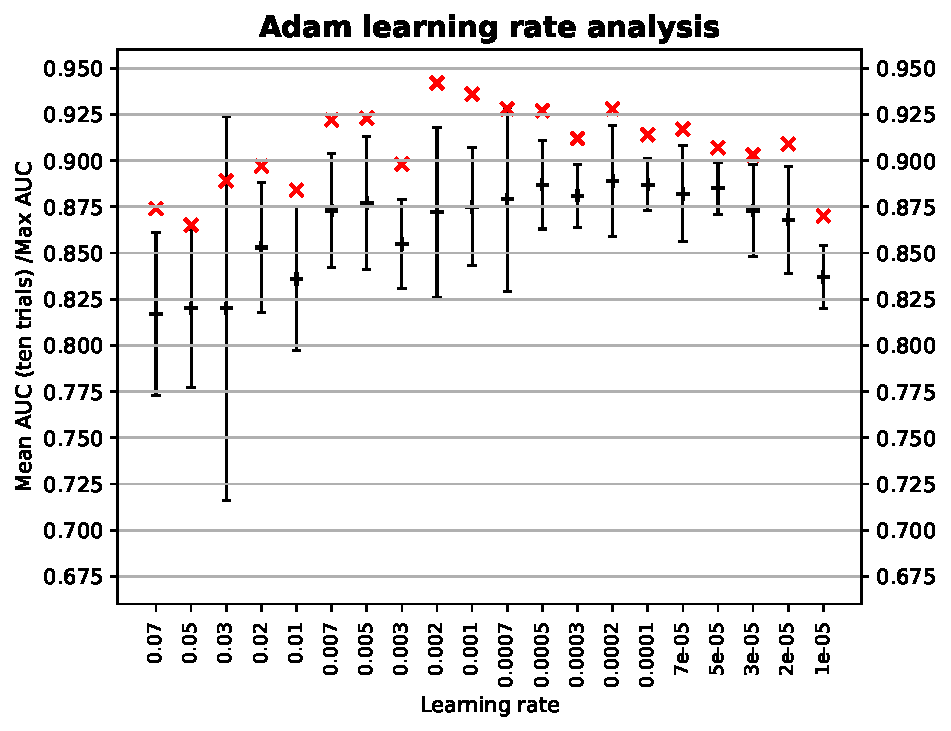
\includegraphics[width=.4\textwidth]{images/densenet/siamese/densenet_siamese_adam_lr}\quad
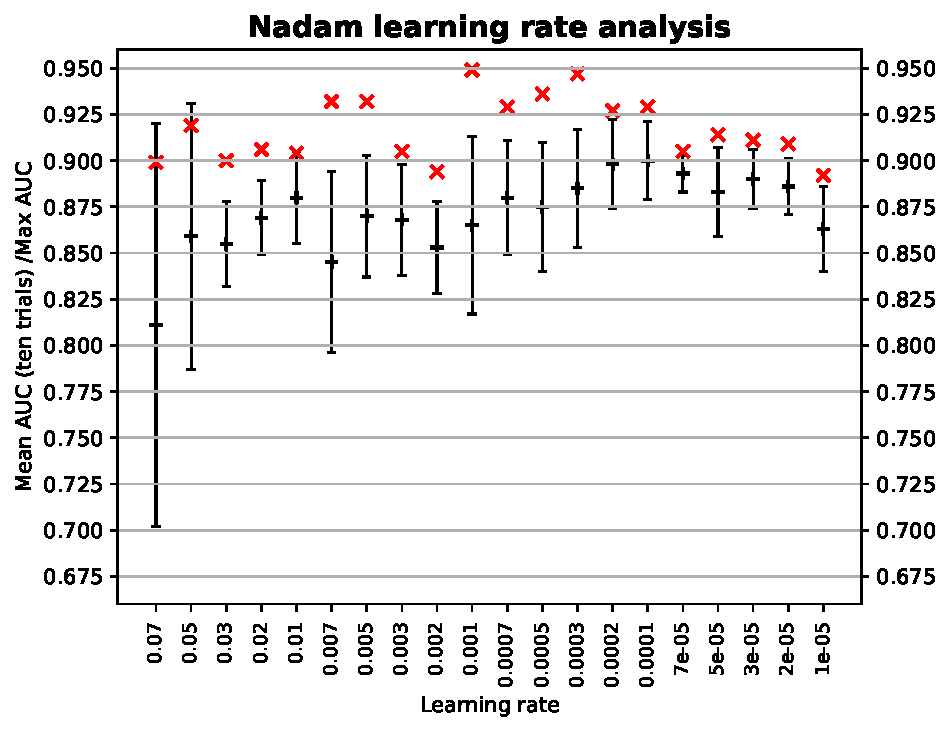
\includegraphics[width=.4\textwidth]{images/densenet/siamese/densenet_siamese_nadam_lr}

\medskip
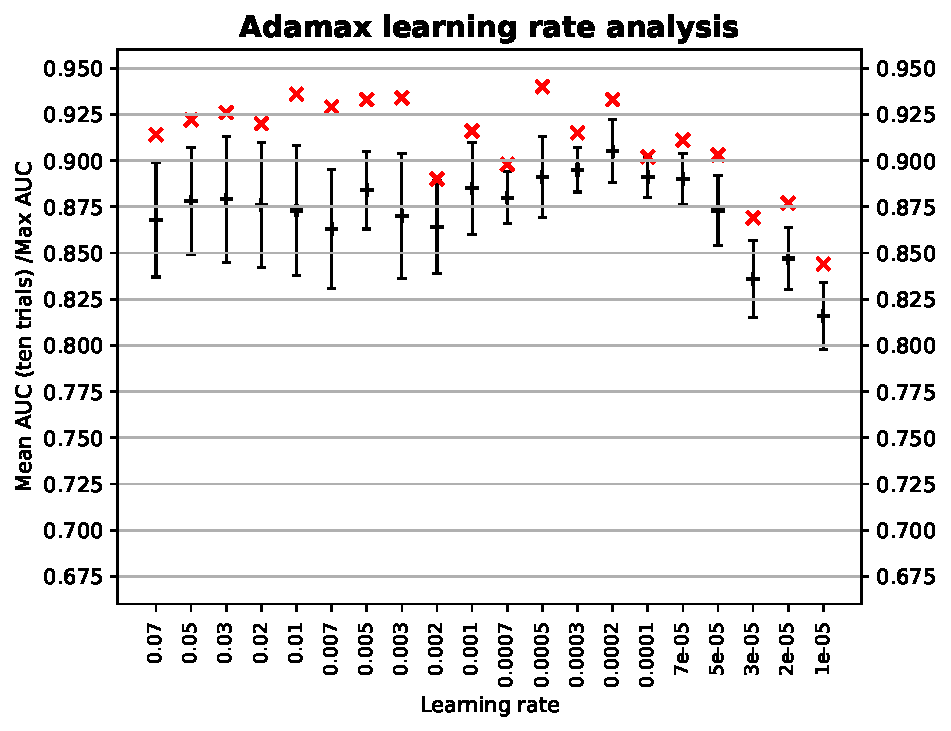
\includegraphics[width=.4\textwidth]{images/densenet/siamese/densenet_siamese_adamax_lr}\quad
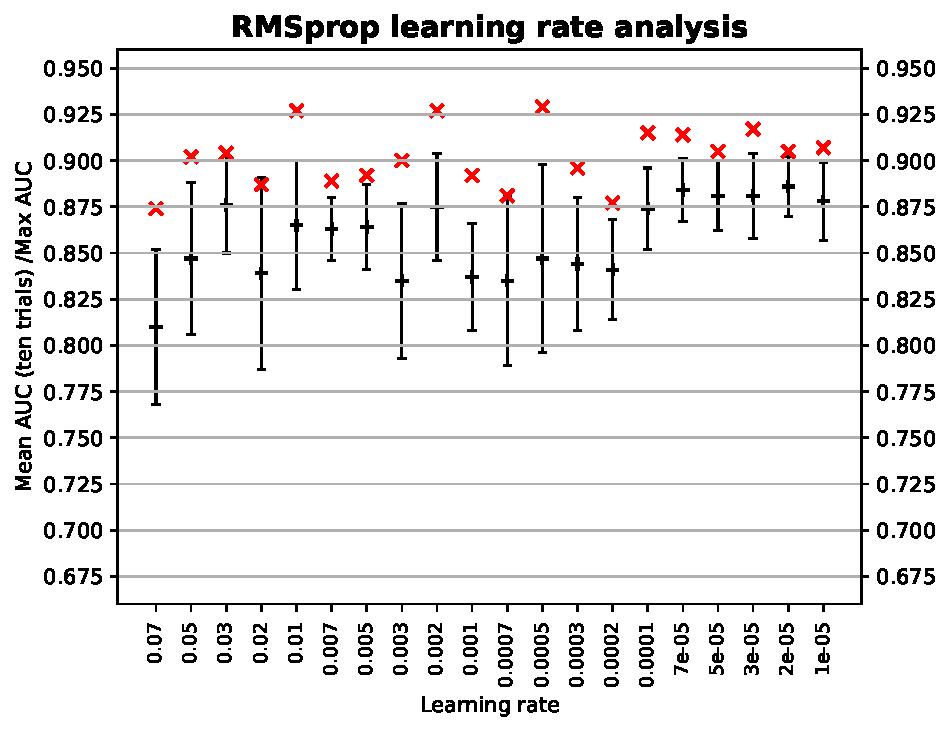
\includegraphics[width=.4\textwidth]{images/densenet/siamese/densenet_siamese_rmsprop_lr}

\medskip
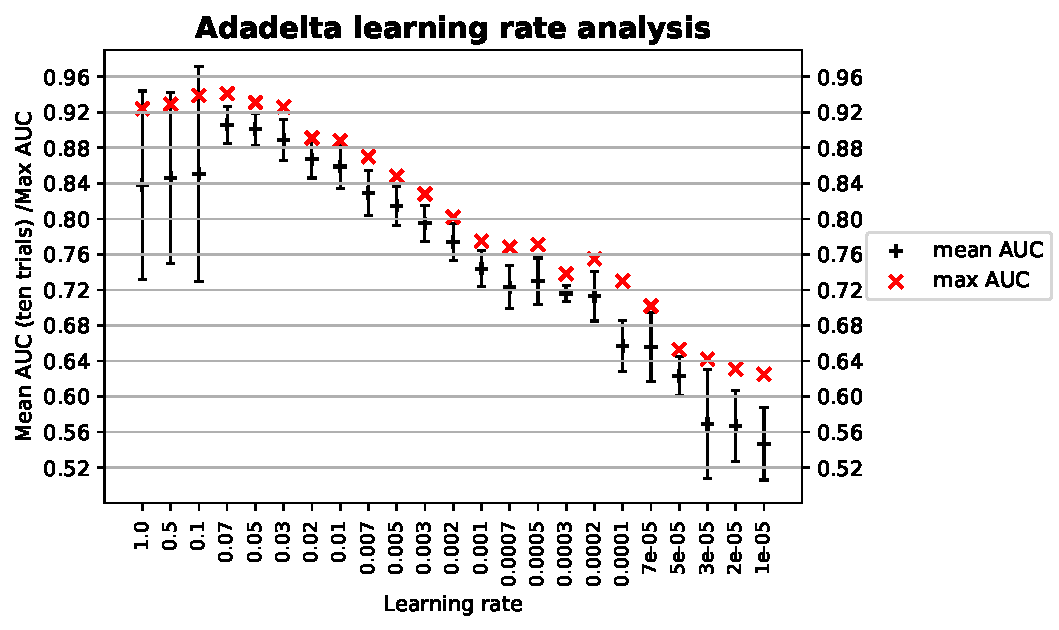
\includegraphics[width=7cm,height=5cm]{images/densenet/siamese/densenet_siamese_adadelta_lr}

\caption{In order, (a)Adam, (b)Nadam, (c)Adamax, (d)RMSprop, (e)Adadelta learning rate analysis}
\label{fig:lr_optimizers}
\end{figure}

\begin{figure}[ht]
\centering
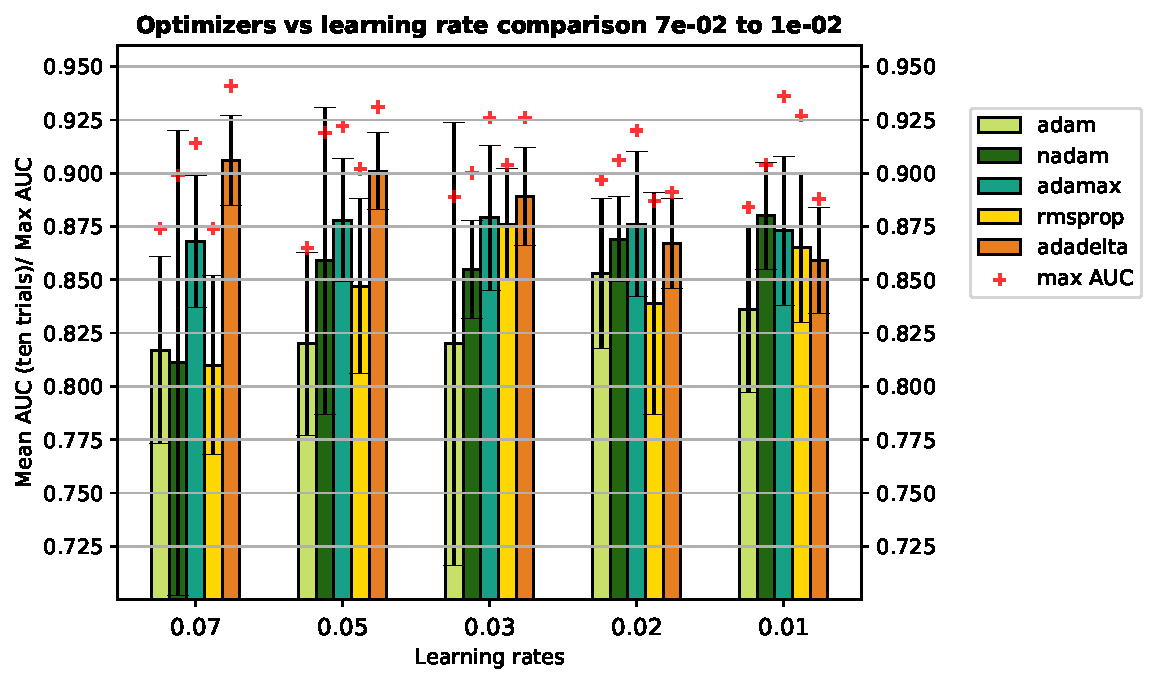
\includegraphics[width=7cm]{images/densenet/siamese/densenet_siamese_lr1_bar}\quad
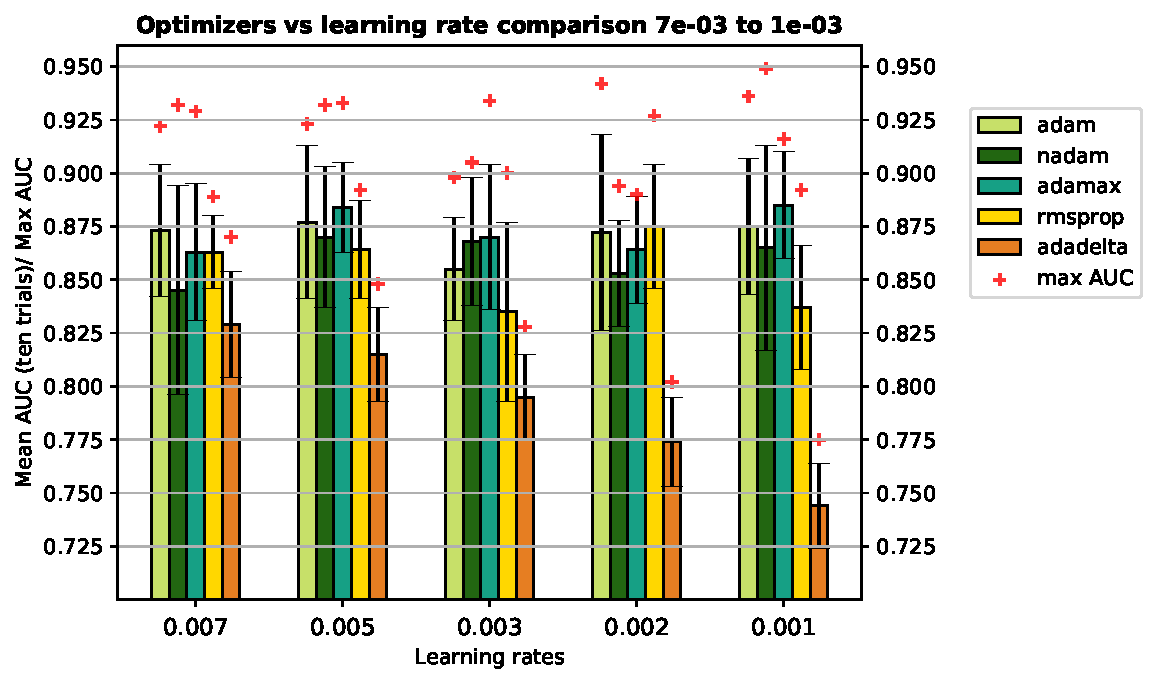
\includegraphics[width=7cm]{images/densenet/siamese/densenet_siamese_lr2_bar}

\medskip
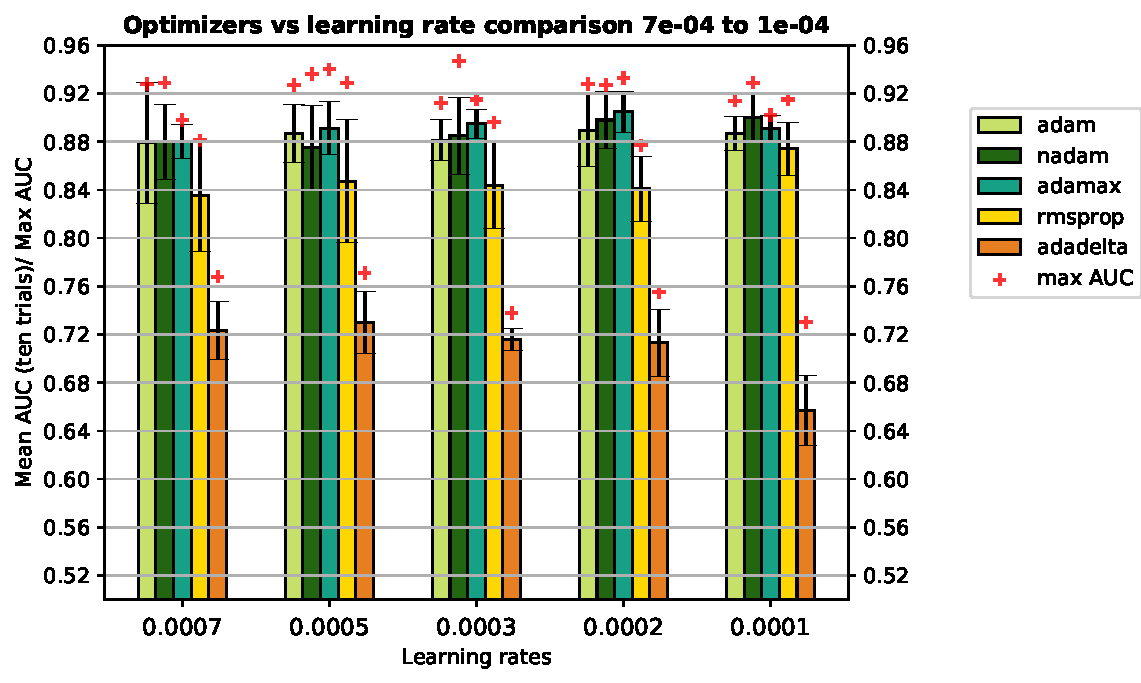
\includegraphics[width=7cm]{images/densenet/siamese/densenet_siamese_lr3_bar}\quad
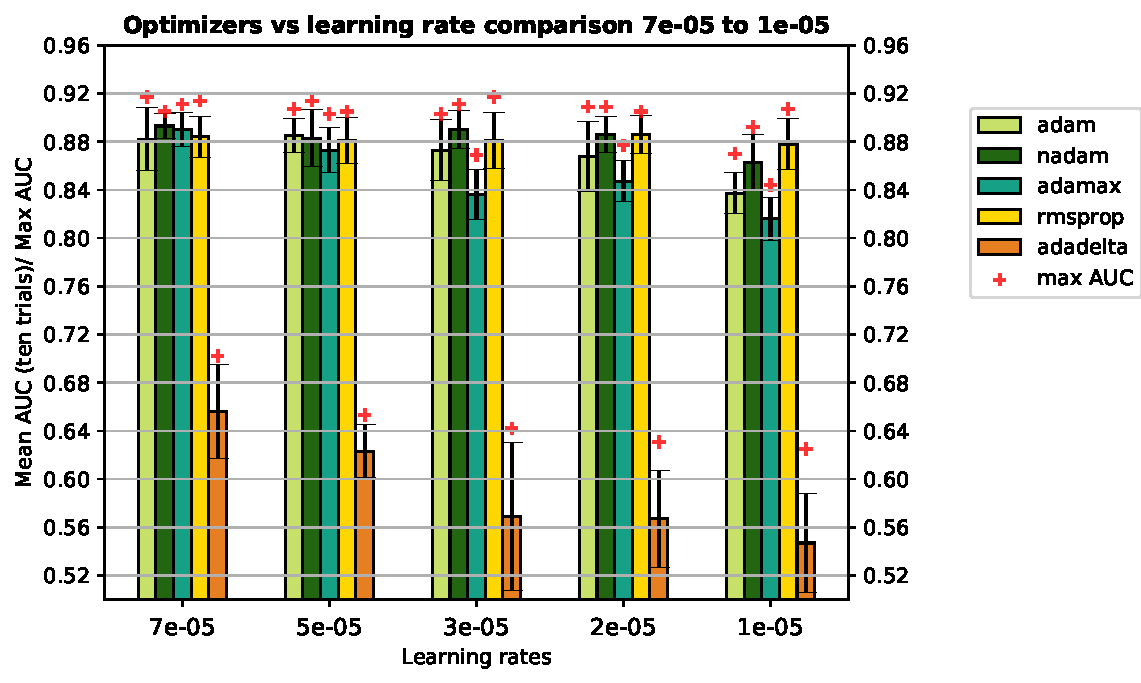
\includegraphics[width=7cm]{images/densenet/siamese/densenet_siamese_lr4_bar}

\caption[Comparison of different optimizers across different learning rates.]{Comparison of different optimizers across different learning rates. For more effective comparison the total evaluation is visualized 5 learning rate at a time. 
Mean AUC obtained for all five optimizers for specific learning rate are grouped together, visualized using bars of different colors. Each two figures in a row have same limits for comparison.}
\label{fig:lr_optimizers_compare}
\end{figure}


\paragraph{Discussion\\}
Overall Adadelta optimizer with learning rate 0.07 has the highest mean AUC 0.906. Which is closely followed by Adamax and Nadam. Adam and RMSprop are slightly behind. The best mean AUC results are displayed 
in table \ref{table:best_optimizers}. So there is no fixed learning rate for which all the optimizer works best, which is expected as well. For Adamax, Adam, Nadam learning rate 0.0002 works very good, for RMSprop learning rate 2E-5 works better. 
For Adadelta, as the learning rate drops the performance also drops significantly. For Adadelta the best learning rate is at the boundary condition (0.07) of the evaluation range. So further analysis needs to be done for higher learning 
rates like 0.1, 0.5, 1.0. In Keras the default learning rate for Adadelta in Keras is 1.0 so it is not really surprising. 

\begin{table}[htb]
 \centering
 \caption{The learning rate for which the optimizers recorded it's best mean AUC.}
 \begin{tabular}{|c c c|} 
 \hline\hline
 \rowcolor{lightgrey}
 Optimizer & Learning rate & Mean AUC(10 trials) \\ [0.5ex] 
 \hline
 Adadelta & 0.07 & 0.906 \\
 \hline
 Adamax & 0.0002 & 0.905 \\
 \hline
 Nadam & 0.0001 & 0.9 \\
 \hline
 Adam & 0.0002 & 0.889 \\
 \hline 
 RMSprop & 0.00002 & 0.886\\
 \hline \hline
\end{tabular}
\label{table:best_optimizers}
\end{table}

\begin{figure}[htp]
\centering
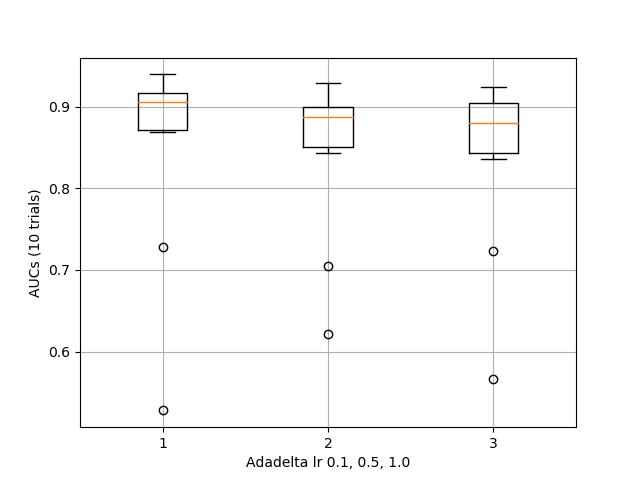
\includegraphics[height=7cm,height=5cm]{images/densenet/adadelta_highlr_analysis}
\caption[Adadelta evaluation for high learning rates.]{Adadelta evaluation for high learning rates. Two of the AUCs out of ten trials for each of the three configurations are displayed as the outlier in the Boxplot. 
In each of the cases the network did not train well and possibly remained stuck in local minima. The Boxplot displays statistical five number summary for the 10 AUCs recorded for each of the configurations.}
\label{fig:adadelta_highlr_analysis}
\end{figure}

\flushbottom
\newpage
From figure \ref{fig:adadelta_highlr_analysis} it is observed that each of the trials with learning rate 0.1, 0.5 and 
1.0 somehow has 2 AUCs out of 10, which are far lower than others. Which are displayed in the boxplot as the outliers. After discarding the outliers the mean AUC of the trials would drastically improve and displayed in the following table 
\ref{table:adadelta_high_lr}. It is however debatable, not fair to calculate mean AUC discarding some runs. In any case best learning rate 0.07 is chosen for Adadelta as it is found to be more dependable and high scoring too.

\begin{table}[ht]
 \centering
 \caption{Optimizer Adadelta evaluation with high learning rates. Displayed results are after filtering the outlier cases.}
 \begin{tabular}{|c c c c c|} 
 \hline\hline
 \rowcolor{lightgrey}
 Learning rate & 0.07 & 0.1 & 0.5 & 1.0 \\ [0.5ex] 
 \hline
 Mean AUC & 0.906 & 0.906 & 0.891 & 0.887 \\ 
 \hline \hline
\end{tabular}
\label{table:adadelta_high_lr}
\end{table}


\subsection{DenseNet-Siamese Final Grid Search}
The search for the best hyperparameters are done separately so far, now all the best performing hyperparameter values are put together as part of this final grid search. If the hyperparameters that are searched separately, did 
not have any interdependency (e.g., Learning rate and optimizer has), then the overall prediction accuracy should improve when all the best hyperparameter values are used together. 

\subsubsection{Hyperparameters For Final Grid Search}
The search space for this final grid search has been narrowed 
down manifold by doing the individual or focused parameter search before. The remaining search space for the final search is described below in table \ref{table:final_run_search_space}.

\begin{table}[ht]
\centering
\caption{Best hyperparameter values for final evaluation.}
\resizebox{\textwidth}{!}
{\begin{tabular}{|l c| l c| l c|} 
 \hline\hline
 \rowcolor{lightgrey}
 \multicolumn{1}{|c}{\textbf{Name}} & \multicolumn{1}{c|}{\textbf{Value}} & \multicolumn{1}{c}{\textbf{Name}} & \multicolumn{1}{c|}{\textbf{Value}} & \multicolumn{1}{c}{\textbf{Name}} & \multicolumn{1}{c|}{\textbf{Value}} \\ [0.5ex] 
 %Name & Value & Name & Value & Name & Value\\ [0.5ex] 
 \hline
 Number of filter & 16 & Layers & 2-2, 3-4 & Growth rate & 12, 18, 30\\
 \hline
 DenseNet dropout & 0.2, 0.4 & Compression & 0.3, 0.7 & Bottleneck & 'False'\\
 \hline
 FC output & 512 & FC dropout & 0.5, 0.7 & Pooling & 'flatten' \\
 \hline
 Batch size & 64 & Optimizer \& learning rate & \multicolumn{3}{c|}{'Adadelta' \& 0.07, 'Adamax' \& 0.0002, 'Nadam' \& 0.0001} \\
 \hline \hline
\end{tabular}}
\label{table:final_run_search_space}
\end{table}

From the table \ref{table:final_run_search_space}, it is observable that three different optimizers are evaluated with their corresponding learning rates. So basically each test case is evaluated for each optimizer.
Similarly for other hyperparameters, which have more than one values in the search space, the overall search cases are multiplied by the number of those many values. Here total of 48 x 3 (for optimizers) = 144 dimensional search space is 
being searched for the final evaluation i.e 144 network configurations. Each of them will be trained from scratch 10 times and the network configuration with best mean AUC for test data prediction, is considered to be the best network. 
And the corresponding hyperparameter values will be the best hyperparameter values for DenseNet-Siamese network.

%\textbf{Top config 1 Adadelta}\\
%Epochs 14 batch\_size: 64 lr: 0.07 optimizer: adadelta \\
%es\_patience: 4 lr\_patience: 3\\
%batch\_size: 64 fc\_dropout: 0.7 fc\_filter: 512 fc\_layers: 1 \\
%Layers: [2, 2] Growth\_rate: 30 \\
%nb\_filter: 16 dropout: 0.4 dense\_block 2 \\
%reduction\_: 0.3 bottleneck: False \\

\begin{table}[ht]
\centering
\caption[Best hyperparameter values for the DenseNet-Siamese ...]{Best hyperparameter values for the DenseNet-Siamese, obtained from the final grid search. In decreasing order of their mean prediction accuracy on the test data. 
The results are very close, hence top 5 results are displayed instead of just one.}
\resizebox{\textwidth}{!}
{\begin{tabular}{|c c c l c c c c c c c|} 
 \hline\hline
 \rowcolor{lightgrey}
\textbf{Config alias} & \textbf{Epochs} & \textbf{Learning rate} & \textbf{Optimizer} & \textbf{Layers} & \textbf{Growth rate} & \textbf{DenseNet dropout} & \textbf{Compression} & \textbf{Mean AUC} & \textbf{Std} & \textbf{Max AUC}\\
\hline
'Config 1' & 14 & 0.07 & 'Adadelta' & 2-2 & 30 & 0.4 & 0.3 & 0.921 & 0.016 & 0.95 \\
'Config 2' & 15 & 0.0002 & 'Adamax' & 2-2 & 18 & 0.4 & 0.7 & 0.918 & 0.009 & 0.935\\
'Config 3' & 14 & 0.07 & 'Adadelta' & 3-4 & 12 & 0.4 & 0.7 & 0.915 & 0.019 & 0.94\\
'Config 4' & 14 & 0.07 & 'Adadelta' & 2-2 & 18 & 0.4 & 0.3 & 0.913 & 0.012 & 0.927\\
'Config 5' & 13 & 0.07 & 'Adadelta' & 2-2 & 12 & 0.2 & 0.7 & 0.912 & 0.011 & 0.932\\
 \hline \hline
\end{tabular}}
\label{table:final_run_best_configs}
\end{table}

\flushbottom
\newpage
All the top results were obtained for FC dropout probability 0.7. Other hyperparameters which has multiple values in final search space, the best values are mentioned in table \ref{table:final_run_best_configs}. Rest of the hyperparameter values are fixed to what is displayed in table \ref{table:final_run_search_space}. 
From table \ref{table:final_run_best_configs} the 'Config aliases' are used to refer to the network structure in the following figures, for comparing the results.

\begin{figure}[ht]
\centering
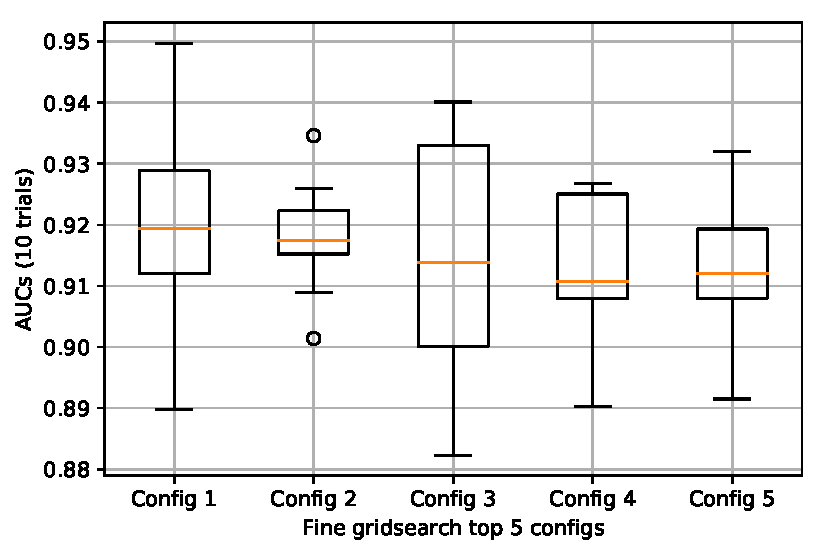
\includegraphics[height= 5cm]{images/densenet/siamese/top_config_boxplot}
\caption[Boxplot visualization of top five DenseNet-Siamese network]{Top five DenseNet-Siamese network each evaluated 10 times from scratch. For most effectively compare the network statistical analysis is done for all ten AUC prediction results
for each of the network and visualized using Boxplot}
\label{fig:fine_grid_search_top_configs}
\end{figure}

\begin{figure}[ht]
\centering
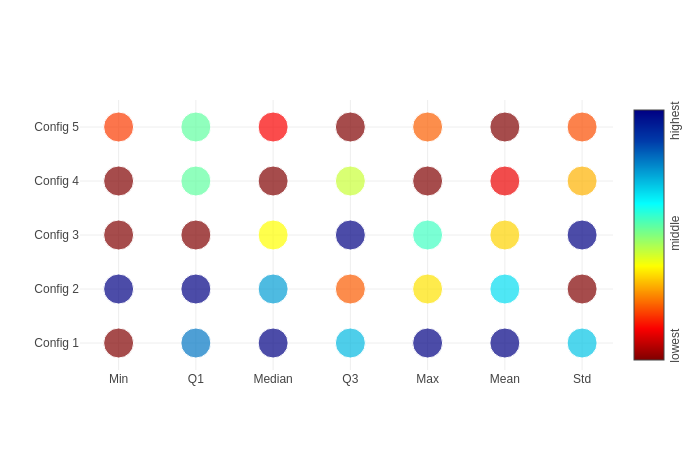
\includegraphics[height= 7cm]{images/densenet/siamese/top5_final_bubble_compare}
\caption[Top five network statistical comparison in bubble plot]{Statistical analysis on top results from final grid search visualized in bubbles with color codes which enable the qualitative analysis among different configurations.}
\label{fig:top5_analysis_bubble}
\end{figure}

%\flushbottom
%\newpage

\paragraph{Discussion\\}
The best result reported in Valdenegro-Toro \cite{stateoftheart} is \textbf{0.91} AUC for binary class prediction and \textbf{0.894} for the score prediction, for the same data used in this thesis. However, 
In this work only score prediction is done. DenseNet-Siamese network able to record highest mean AUC in ten trials \textbf{0.921}, with standard deviation across the trials of 0.016 and maximum AUC of 0.950. 
Which is higher than the state of the art score prediction.
The best performance is recorded with Adadelta optimizer and learning rate 0.07. %What about the rest of the configs?

The mean AUC result for the top configurations are very close and it is hard to declare a runaway winner as the highest network has mean AUC of 0.921 and std of 0.016, second best has mean AUC of 0.918 with std 0.009. 

It is interesting to note that the dropout values which are giving the best results are high 0.7 for the Siamese side and 0.4 (only for 'Config 5' it is 0.2) for the DenseNet side. 
High dropout is enabling the network to be good in generalization. The training/validation accuracy is could reach very high, still the generalization on test data is high.

The statistical comparison of the evaluations which yielded top 5 mean AUC are displayed in figure \ref{fig:fine_grid_search_top_configs}. Each of the 5 network configuration is evaluated for 10 times and the prediction accuracies 
are compared quantitatively based on the box and whisker plot representation.

Interestingly enough, for 'Config 2', two points are displayed to lie out side the boxes. This supposed outliers, both in higher and lower end of the distribution range, are not really outliers, it just so happens that this 
two values are bit higher and lower than the rest 8 Auc values, which have only standard deviation of only 0.05. In fact this shows that this result is the most consistent one, it is also the only top configuration that uses 'Adamax' 
optimizer and as seen from the \ref{table:final_run_best_configs} the reduction ratio is 0.7. In comparison to the 'Config 1' the reduction ratio used for 'Config 2' is higher. As previously seen in figure 
\ref{fig:compression_and_bn_vs_parameters} the total parameters for the networks are much lesser for the 'Config 2' than 'Config 1'. So overall this result for 'Config 2' is also very good.


And in figure \ref{fig:top5_analysis_bubble} multiple statistical data is displayed in bubbles 
whose color indicates the scale of the value. Lowest values indicated by brown or shade of red and as it gets higher the color gets orange, yellow, green, cyan to blue and darker blue. Each column may have data in different ranges, 
so for most effective qualitative comparison each columns, which are one of the statistical measure, the color maps normalized for each of the column. It is done automatically, by assigning the lowest value of the 5 results for each metric
to the lowest color map and highest to the highest color map. So in this one image \ref{fig:top5_analysis_bubble} results from 50 evaluations are summarized. That is 10 evaluations for each of the 5 network configurations. 
The visualization displays statistical five number summary (min, Q1, median, Q3, max) and mean and standard deviation are computed from each of the 10 evaluations for each configuration, which signifies how each network performs. 

This visualization is intended for rough qualitative analysis among the top configurations. It is clear that the 'Config 1' network outperforms other networks, because overall it has most 'bubbles' which are blue or dark blue,
which means high values. Except the min value is very low, it's displayed in brown. Similarly,'Config 2' is also very good. 
It has the lowest standard of deviation. Apart from this configuration (with 'Adamax'), other four top configurations are using 'Adadelta'. 'Nadam' has got the best mean AUC of 0.912, which is same as the 'Config 5'. 
In figure \ref{fig:auc_top_config} the Receiver operating characteristic (ROC) curve is presented for the best network 'Config 1'. The ROC curve is based on the evaluation which has maximum accuracy out of 10 runs for 'Config 1'.
With this results the hyperparameter search for DenseNet-Siamese comes to the conclusion.

\begin{figure}[ht]
\centering
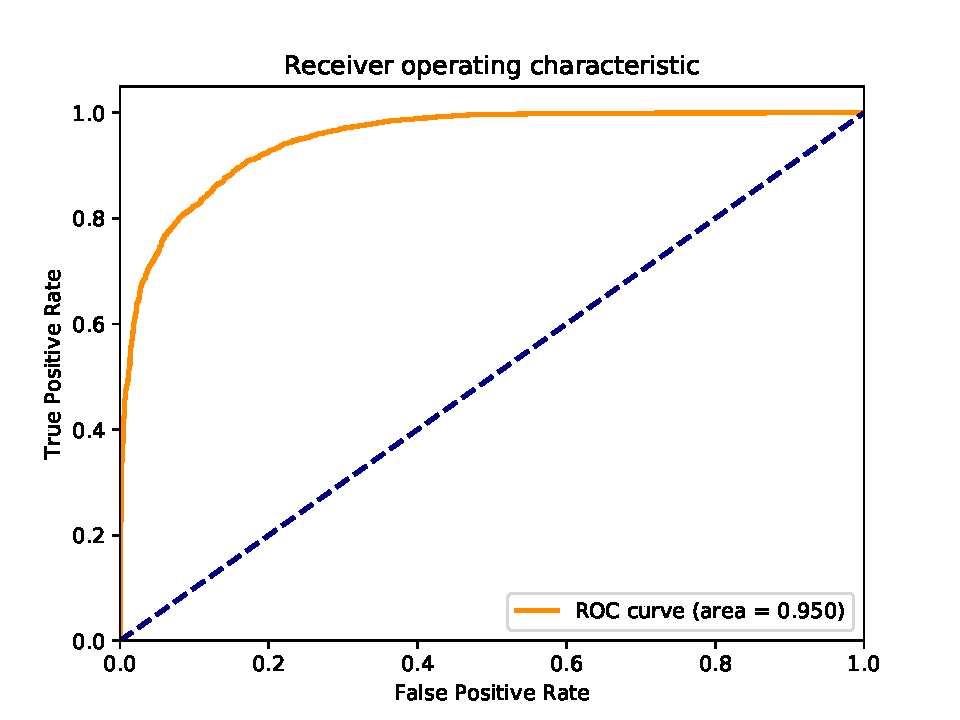
\includegraphics[height= 5cm]{images/densenet/siamese/keras_densenet_siamese_4Nov_15400_9497}
\caption[Area under curve for best Config 1]{The area under curve is visualized for the best network 'Config 1'.}
\label{fig:auc_top_config}
\end{figure}


%\flushbottom
%\newpage

\section{DenseNet Two-Channel}
\label{section:densenet}

In order to get the best result from DenseNet two-channel \textbf{(DTC)} network for the dataset used in this work, best hyperparameter values needs to be found out. 
In the following section how the best hyperparameter search for DTC is conducted is described. Also the result of the DTC using the best parameter values are evaluated and the results are visualized for easier interpretation.

\subsection{DenseNet Two-Channel Hyperparameters To Be Evaluated}
Overall hyperparameters of DTC can be divided into divided into two parts as follows:
\subsubsection{Hyperparameters Of DenseNet}
This important hyperparameters are already mentioned in the section \ref{hyperDenseNet}, during the best hyperparameter search for DenseNet-Siamese. While the structure and the intended functional usage are different the DenseNet two-channel
and DenseNet-Siamese both depend on the basic feature extraction capability of the network. Hence there are some common knowledge which can be extracted from the hyperparameter search in previous section (DenseNet-Siamese network). But the main 
hyperparameters such as growth rate, layers per block, number of filters, reduction and bottleneck still needs to be searched again, as the network structure is different.

\subsubsection{Other Hyperparameters}
Apart from the DenseNet there are other general hyperparameters such as learning rate, batch size for training and optimizer. 

%\subsubsection{Grid search strategy}
%Since there are lot of parameters, practically, infinite test cases might be designed. To keep the grid search focused and less computationally expensive it makes sense to 
%first search for coarser grid of parameters rather than very fine ones. When and if a bracket of parameters are shortlisted which works better than others, the finer parameter
%earch will be performed only specific to those range of parameters and not the whole grid.

\subsection{DenseNet Growth Rate And Layers Per Block Analysis}

Similar to the previous analysis, once all the hyperparameters which needs to be evaluated are known, manual optimization takes place. 
After many trial and error cycles or randomly the parameter values are changed around to get a intuition on the possible ranges for the hyperparameter values to be evaluated. This step also ensures that the starting point is not very bad.
Layers per block are chosen among 2, 3, 4, 5, 6. For single dense block evaluation goes up-to 12 layers (per block). 
Each network has been evaluated for growth rates of 12, 18, 24, 30. Growth rate 6, 36 excluded as they are too thin and too thick respectively (found from DenseNet-Siamese evaluation). Different dense block sizes of 1, 2, 3, 4. 
There are other parameters but number of dense block, growth rate and layers per block are three main parameters. The parameters compression/reduction and bottleneck are set 0.5 and False respectively. 
For more fine grained analysis the reduction and bottleneck parameters might be evaluated. \code{nb\_filter} values are fixed at 16 for this test. The parameter classes are set to 2, where class 1 for matching patches and 0 
for not-matching patches. 96, 96 is the input image dimensions and input is two-channel. So depending on local setting of the keras, “channel-first” or “channel-last” suitable input\_shape is 
chosen automatically as 2, 96, 96 or 96, 96, 2 respectively. The learning rate used for the test is 0.07 and Adadelta as optimizer. Best performing combination from DenseNet-Siamese analysis. 
Dropout for DenseNet used as 0.2 to incorporate minimal regularization. Epochs are different for different architectures to ensure that the networks are able to train decently. 
Flatten is used as pooling at the end of the DenseNet, in place of global average pooling. Binary\_crossentropy loss function with Sigmoid activation function used for the binary classification, this final layer acts as the binary classifier.
This is ensured by including the top of DenseNet architecture (\code{include\_top=True}). In all the cases the networks are being trained from scratch. Parameter \code{weights} value None ensures that no previously trained weights are used.

\subsubsection{Growth Rate And Layers Per Block Search Setup Summary}
The overall search space is summarized in the section below.
\subsubsection{Fixed Hyperparameters}
\label{fixed_params}
Other hyperparameters that are needed to instantiate the DenseNet are set to fixed values, in order to focus on the layers per block and growth rate parameters.

\begin{table}[ht]
\centering
\caption{Fixed hyperparameter values for the evaluation setup.}
\resizebox{\textwidth}{!}
{\begin{tabular}{|l c| l c| l c|} 
 \hline\hline
 \rowcolor{lightgrey}
 \multicolumn{1}{|c}{\textbf{Name}} & \multicolumn{1}{c|}{\textbf{Value}} & \multicolumn{1}{c}{\textbf{Name}} & \multicolumn{1}{c|}{\textbf{Value}} & \multicolumn{1}{c}{\textbf{Name}} & \multicolumn{1}{c|}{\textbf{Value}} \\ [0.5ex] 
 \hline
 Number of filter & 16 & Subsample initial block & 'True' & Weights & 'None'\\
 \hline
 Dropout rate & 0.2 & Include top & 'True' & Compression & 0.5\\
 \hline
 Bottleneck & 'False' & Pooling & 'flatten' & Transition pooling & 'max' \\
 \hline
 Optimizer & 'adadelta' & Learning rate & 0.07 & & \\
 \hline \hline
\end{tabular}}
\label{table:architecture_densenet_siamese}
\end{table}

\subsubsection{Varying Hyperparameters}

 \begin{itemize}
 \item \textbf{Nb\_layers\_per\_block}:
 \begin{itemize}
  \item \textbf{One dense block architecture (nb\_dense\_block=1)}\\
  '2', '4', '6', '8', '10', '12'
  \item \textbf{Two dense block architecture (nb\_dense\_block=2)}\\
  '2-2', '4-4', '6-6'
  \item \textbf{Three dense block architecture (nb\_dense\_block=3)}\\
  '2-2-2', '4-4-4', '6-6-6'
  \item \textbf{Four dense block architecture (nb\_dense\_block=4)}\\
  '2-2-2-2', '4-4-4-4', '6-6-6-6'
 \end{itemize}
 \item \textbf{Growth rate}:
 \begin{itemize}
 \item Thin layers: 12, 18
 \item Thick layers: 24, 30  
 \end{itemize} 
\end{itemize}
 
\flushbottom
\newpage

%\subsubsection{Architecture analysis}
\begin{figure}
  \centering
  \begin{subfigure}[b]{7cm}
    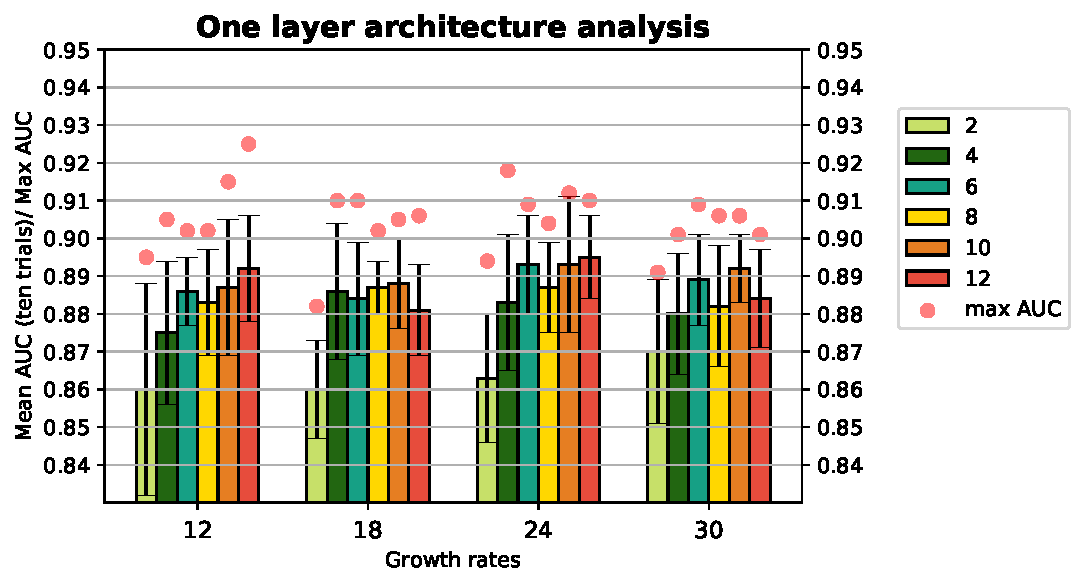
\includegraphics[width=\textwidth]{images/densenet/simple/densenet_simple_single_layer_bar}
    \caption{Single layer }
    \label{fig:densenet_simple_single_layer_bar}
  \end{subfigure}
  ~ %add desired spacing between images, e. g. ~, \quad, \qquad, \hfill etc. 
   %(or a blank line to force the subfigure onto a new line)
  \begin{subfigure}[b]{7cm}
    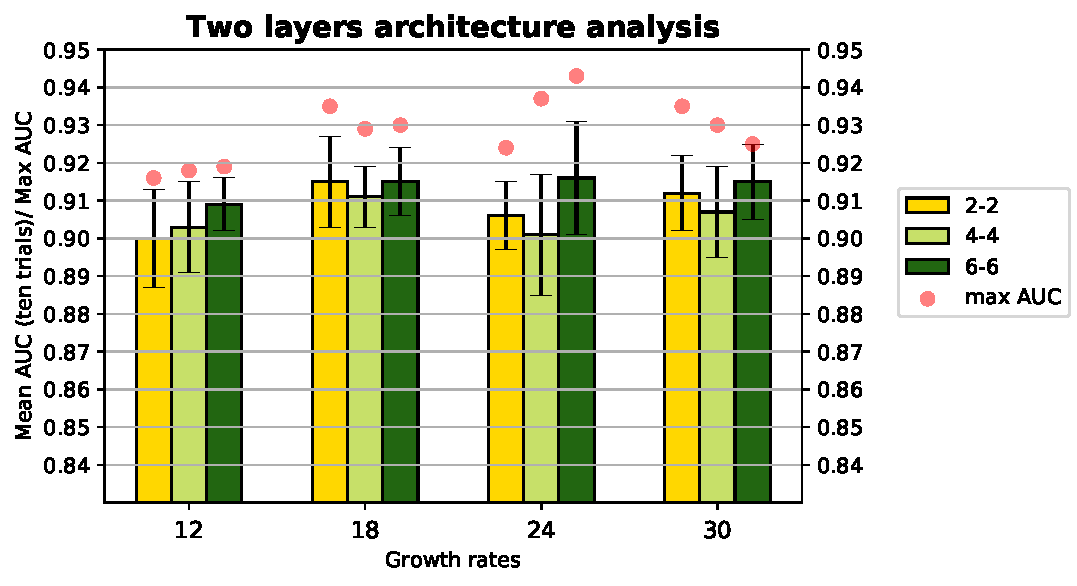
\includegraphics[width=\textwidth]{images/densenet/simple/densenet_simple_double_layer_bar}
    \caption{Two layers}
    \label{fig:densenet_simple_double_layer_bar}
  \end{subfigure}  
  \quad
  \centering
  \begin{subfigure}[b]{7cm}
    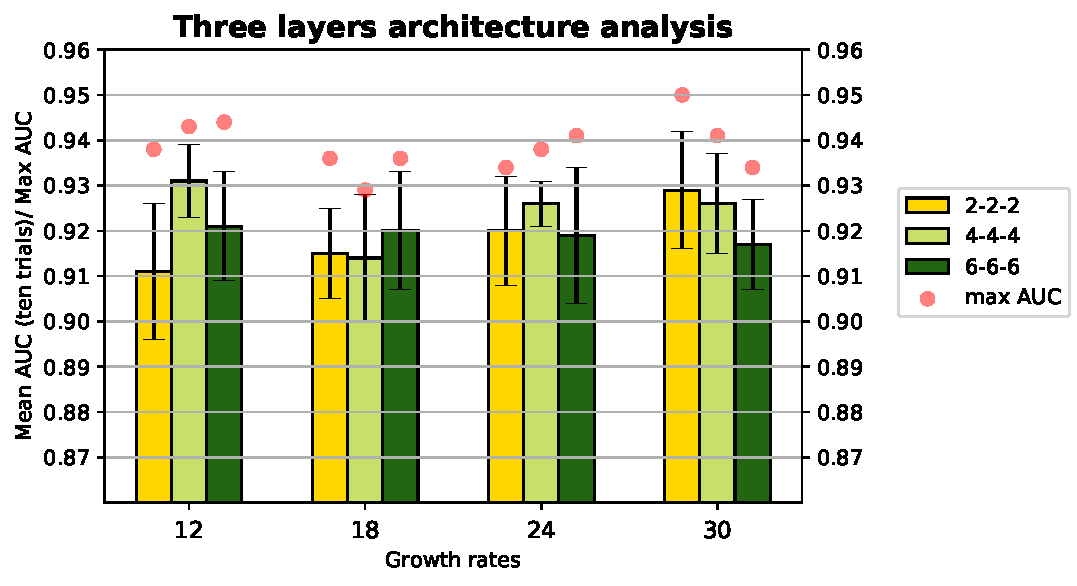
\includegraphics[width=\textwidth]{images/densenet/simple/densenet_simple_three_layer_bar}
    \caption{Three layers }
    \label{fig:densenet_simple_three_layer_bar}
  \end{subfigure}
  ~ %add desired spacing between images, e. g. ~, \quad, \qquad, \hfill etc. 
   %(or a blank line to force the subfigure onto a new line)
  \begin{subfigure}[b]{7cm}
    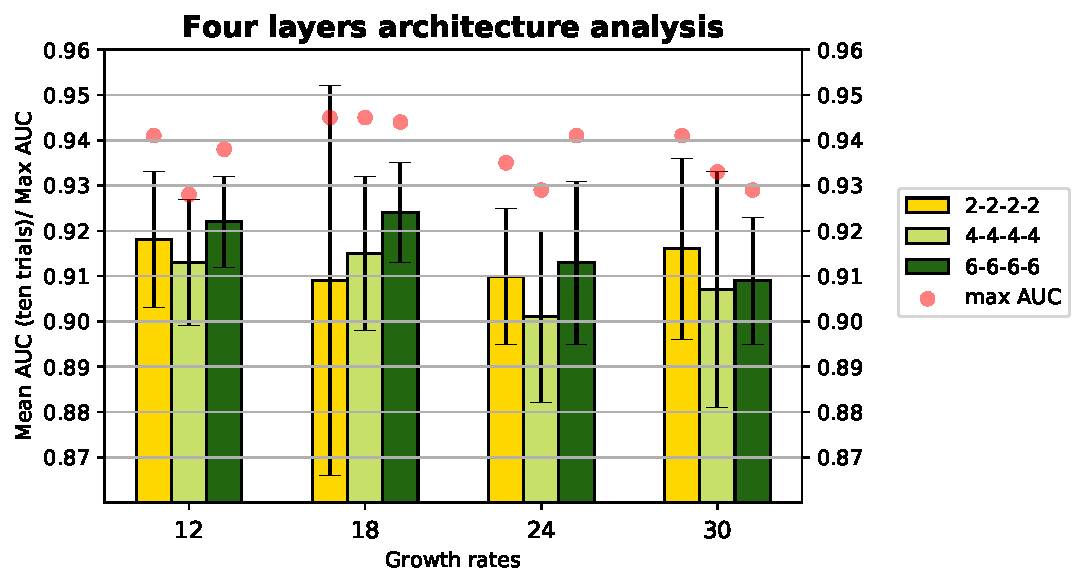
\includegraphics[width=\textwidth]{images/densenet/simple/densenet_simple_four_layer_bar}
    \caption{Four layers}
    \label{fig:densenet_simple_four_layer_bar}
  \end{subfigure} 
  \caption[DenseNet two-channel architecture analysis]{DenseNet two-channel layers per block and growth rate analysis. Unique layers per block is represented with a specific
  color code. Whole result is divided according to dense block numbers, for easier representation. Every two charts presented side by side have identical 
  y-axis for comparison. All the results obtained for same growth rate are grouped together for each of the growth rate (12, 18, 24, 30) represented by x-axis.}
  \label{fig:dense_arch_1}
\end{figure} 

\paragraph{Discussion\\}
Each sub-figure shows mean AUC (on the test dataset) and standard deviation of 10 trials and maximum AUC. From figure \ref{fig:dense_arch_1} it is clear that 4 dense blocks and 3 dense blocks network performs better
than the 1 and 2 block/s networks. The original paper \cite{densenet} also used 3 and 4 blocks DenseNet for most of the evaluations. So this finding is expected. For growth rates though, no clear trend is observed,
in fact, from sub-figure \ref{fig:dense_arch_1}(c) it is observed that with increase in growth rate the '2-2-2' network performs better, while for '6-6-6' it mildly decreasing and similar for '4-4-4'. So no common best growth rate
can not be determined for all the architectures, so it would be safe to evaluate for as many as possible. Growth rate 12, 18 and 30 will be evaluated for the final run. 

\subsection{Pooling Analysis}
The type of pooling used at the end of the network also determines the size of the total parameter size and also affects the generalization of the data. The original paper \cite{densenet} used global average pooling (\code{avg}) \cite{lin2013network}. 
In the previous study \code{flatten} pooling is evaluated, for this analysis \code{avg} pooling is evaluated for 3 layer and 4 layer DenseNet blocks, since they are the best performing network in previous analysis. In figure 
\ref{fig:dense_avg_pooling_1} it is observed that between the three layer and four layers DenseNets, the former performs better. Overall the avg pooling is resulting in smaller total network parameters and also the better mean AUCs.

\begin{figure}
  \centering
  \begin{subfigure}[b]{0.4\textwidth}
    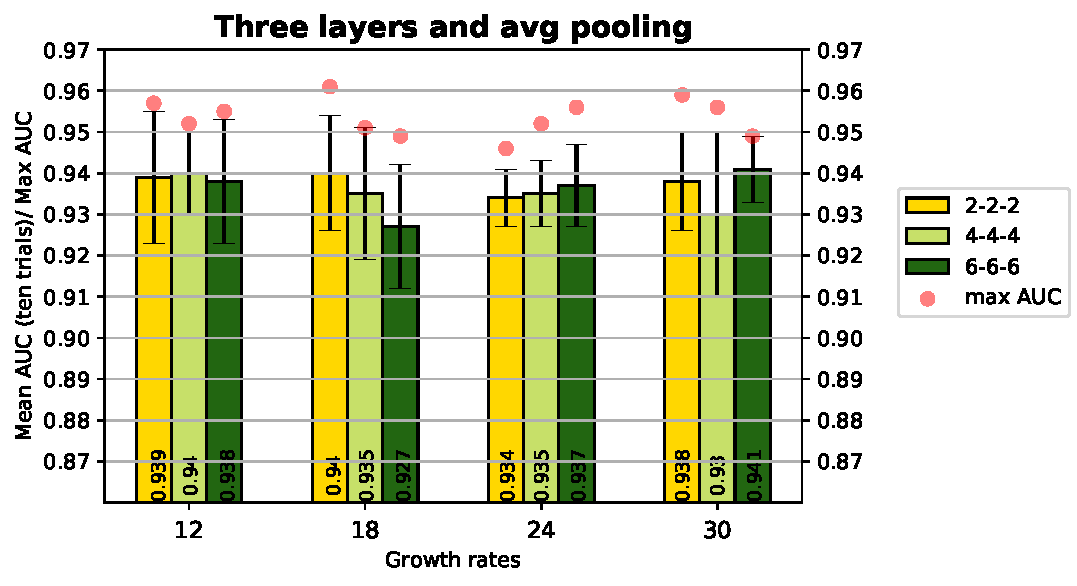
\includegraphics[width=\textwidth]{images/densenet/simple/densenet_simple_three_layer_avg_bar}
    \caption{Three layers avg pooling }
    \label{fig:densenet_simple_three_layer_avg_bar}
  \end{subfigure}
  ~ %add desired spacing between images, e. g. ~, \quad, \qquad, \hfill etc. 
   %(or a blank line to force the subfigure onto a new line)
  \begin{subfigure}[b]{0.4\textwidth}
    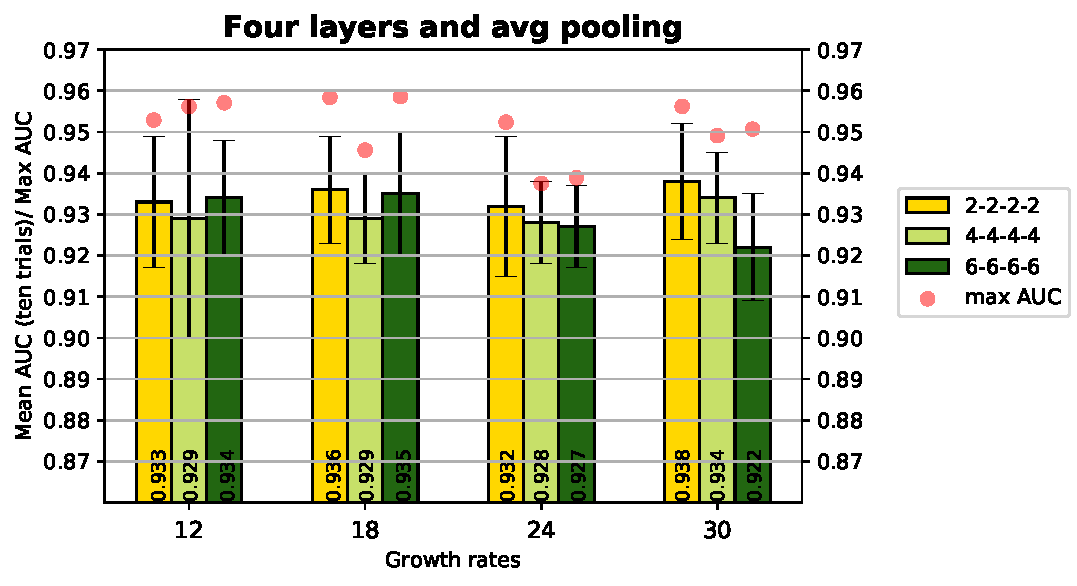
\includegraphics[width=\textwidth]{images/densenet/simple/densenet_simple_four_layer_avg_bar}
    \caption{Four layers avg pooling}
    \label{fig:densenet_simple_four_layer_avg_bar}
  \end{subfigure}    
  \caption{DenseNet two-channel avg pooling analysis}
  \label{fig:dense_avg_pooling_1}
\end{figure}

For a comparative analysis between the flatten and average pooling the mean AUCs are compared for each of the growth rate and for three layers DenseNet (2-2-2, 4-4-4, 6-6-6). Apart this layers and growth rate values, and pooling, 
other parameters remain same as the basic evaluation network \ref{fixed_params}.

\begin{figure}[ht]
\centering
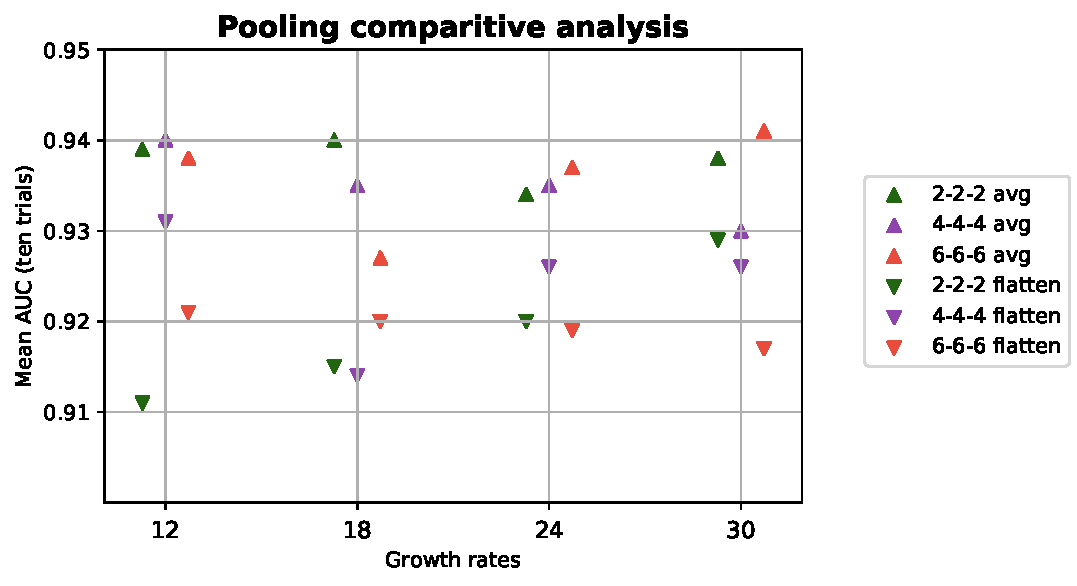
\includegraphics[width=0.5\textwidth]{images/densenet/simple/densenet_simple_three_layer_pooling_compare}
\caption{Average vs flatten pooling}
\label{fig:densenet_simple_three_layer_pooling_compare}
\end{figure}

\paragraph{Discussion\\}
Here, the triangle up represents the mean AUC obtained using average pooling, triangle down represents flatten pooling. The results from the DenseNet
architectures have been grouped together for each growth rates accordingly. So the x-axis of the graph shows growth rates. The y-axis represents the mean AUC obtained from 10 trials of each configurations.
From figure \ref{fig:densenet_simple_three_layer_pooling_compare} it is clearly seen that the average pooling produces better results than using flatten, in all the cases. 
Since the representation might be bit complex, the same data from figure \ref{fig:densenet_simple_three_layer_pooling_compare} is displayed in tabular view (\ref{table:pooling_comparison_across_gr}) as follows.

\begin{table}[ht]
\centering
 \caption[The average and flatten pooling comparison results.]{The average and flatten pooling comparison results.}
\begin{tabular}{|l | c| c| c|} 
 \hline\hline
 \rowcolor{lightgrey}
 Architecture & Growth rate & Mean AUC (Flatten) & Mean AUC (Average)\\[0.5ex]
 \hline
 2-2-2 & 12 & 0.911 & 0.939\\
 2-2-2 & 18 & 0.915 & 0.94\\
 2-2-2 & 24 & 0.92 & 0.934\\
 2-2-2 & 30 & 0.929 & 0.938\\
 4-4-4 & 12 & 0.931 & 0.94\\
 4-4-4 & 18 & 0.914 & 0.935\\
 4-4-4 & 24 & 0.926 & 0.935\\
 4-4-4 & 30 & 0.926 & 0.93\\
 6-6-6 & 12 & 0.921 & 0.938\\
 6-6-6 & 18 & 0.92 & 0.927\\
 6-6-6 & 24 & 0.919 & 0.937\\
 6-6-6 & 30 & 0.917 & 0.941\\ \hline \hline
 \end{tabular}
\label{table:pooling_comparison_across_gr}
\end{table}

\subsection{Basic Network Structure}
For doing effective hyperparameter search, need to evaluate the target parameter with the predefined set of values, while all the other parameters which are not directly related are kept constant. So for this purpose a common 
network structure is defined, which is name 'basic network'. For all the hyperparameter searches, this structure will be the same and only the target hyperparameter values will change.
%The '2-2-2', since it is found to be performing very consistently. Also growth rate, 30 and number of filters, 16
\begin{table}
 \centering
\caption{DenseNet two-channel 'basic network structure' for further hyperparameter search.}
\begin{tabular}{|l | c| c| c| l| c| l | c| c| |l|} 
\hline\hline
 \rowcolor{lightgrey}
 Architecture & Growth rate & Nb\_filter & Dropout & LR. \\ 
 2-2-2 & 30 & 16 & 0.2 & 0.07 \\ 
 \hline
 \rowcolor{lightgrey}
 Optimizer & Reduction & Bottleneck & Batchsize & Pooling\\[0.5ex]
 \hline
 adadelta & 0.5 & FALSE & 64 & avg\\
 \hline \hline
\end{tabular}
\label{basic_dtc_network}
\end{table}

\subsection{Number Of Filter Analysis}
Initial number of filters. 8, 16, 32, 64 are being evaluated here. keeping all other parameters fixed, a comparison between mean AUCs (10 trials) obtained with growth rate 18 and 30 is also done under this analysis. 
To explore if the growth rate and number of filter have any effect on each other.

\begin{figure}[ht]
\centering
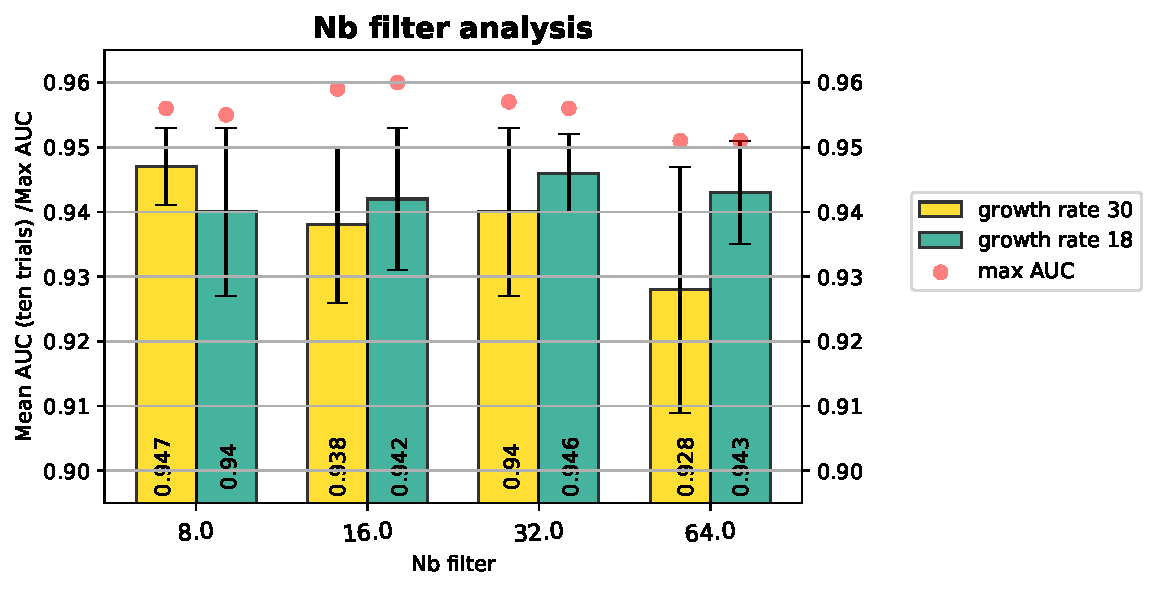
\includegraphics[width=0.5\textwidth]{images/densenet/simple/densenet_simple_nb_filter}
\caption{DTC Number of filter size analysis}
\label{fig:densenet_simple_nb_filter}
\end{figure}

\paragraph{Discussion\\}
It is observed in \ref{fig:densenet_simple_nb_filter} that with change in number of filter size the mean AUC varies a lot for higher growth rate such as 30, for growth rate 18 it does not vary so much. For growth rate 30 the nb 
filter 8 has the best mean AUC. For growth rate 18 the nb filter 32 has the best mean AUC. Overall growth rate 30 with nb filter 8 and growth rate 18 with nb filter 32 are the best combinations.

\subsection{Reduction And Bottleneck Analysis}
This analysis is for evaluating the effect of different reduction ratios and the effect of bottleneck. So the mean AUC is recorded for 10 trials for each of the reduction values 0, 0.2, 0.3, 0.5, 0.7. This is a rather coarser 
search space. But each of them is also evaluated with bottleneck as well, the effect of varying values of reduction and with/without bottleneck is displayed in the figure \ref{fig:densenet_simple_reduction_bottleneck}. 

\begin{figure}[ht]
\centering
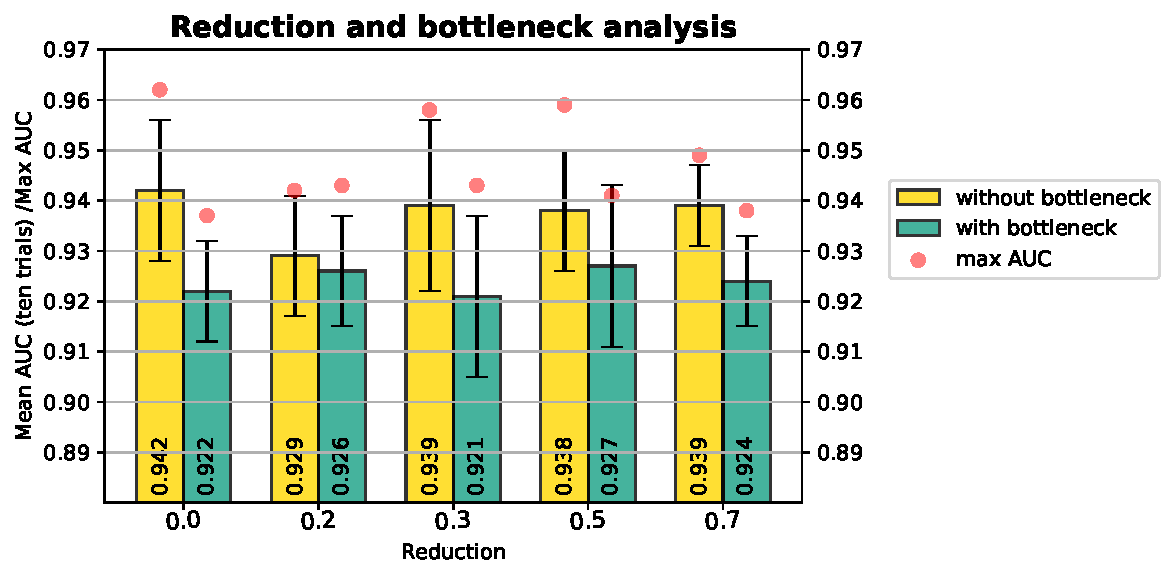
\includegraphics[width=0.5\textwidth]{images/densenet/simple/densenet_simple_reduction_bottleneck}
\caption{Reduction and bottleneck analysis}
\label{fig:densenet_simple_reduction_bottleneck}
\end{figure}

\paragraph{Discussion\\}
The effect of the bottleneck layer is rather limiting the generalization of the network. So it is observed that without bottleneck should be used for future evaluations.
The performance without reduction is best as expected, how ever main purpose of the reduction is to decrease the number of total parameters. The mean AUC are highest and almost same for 0.3, 0.5 and 0.7. The original implementation \cite{densenet} 
uses 0.5 as reduction ratio. Here also 0.5 is selected as the best reduction ratio for the final evaluation.

\subsection{Total Parameters Analysis}
For the total parameter comparison 2, 2-2, 2-2-2, 2-2-2-2 layers per block networks are chosen along with growth rate 18. Every other configurations are kept same, with \code{avg} pooling and without any reduction.
With same configurations, except growth rate, the relation between growth rate and total parameters are evaluated. 

\begin{table}[ht]
\centering
 \caption{Total number of parameters are compared across different number of dense block and different growth rates.}
\begin{tabular}{|l | c | c|} 
 \hline\hline
 \rowcolor{lightgrey}
 Layers per block & Growth rate & Total parameters\\[0.5ex]
 \hline
 2 & 18 & 17217\\
 2-2 & 18 & 47857\\
 2-2-2 & 18 & 96785\\
 2-2-2-2 & 18 & 166593\\
 \hline
 2-2-2 & 12 & 55529\\
2-2-2 & 18 & 96785\\
2-2-2 & 24 & 149201\\
2-2-2 & 30 & 212777\\
 \hline \hline
 \end{tabular}
\label{table:parameter_comparison_dtc}
\end{table}

From \ref{table:parameter_comparison_dtc} it is noted that the total parameters increase as the number of dense blocks increase. Same trend is noted for growth rates too. Total parameters also varies with the choice of pooling and reduction, 
a simple example of each cases is as follows.
Keeping all other configuration same, network has 96785 parameters when \code{avg} pooling is used, and 101685 is the size with \code{flatten} pooling, which is more parameters.
Keeping all other configuration same, with 0.5 reduction ratio for DenseNet the network size goes down to 51430 instead of 96785 total parameters without reduction. Both are evaluated for 2-2-2 layers and growth rate 18.


\subsection{Dropout Probability Analysis}
10 evaluations are done for each test cases, consisting of values ranging between 0 and 0.7, with an interval size of 0.1.
\begin{figure}[ht]
\centering
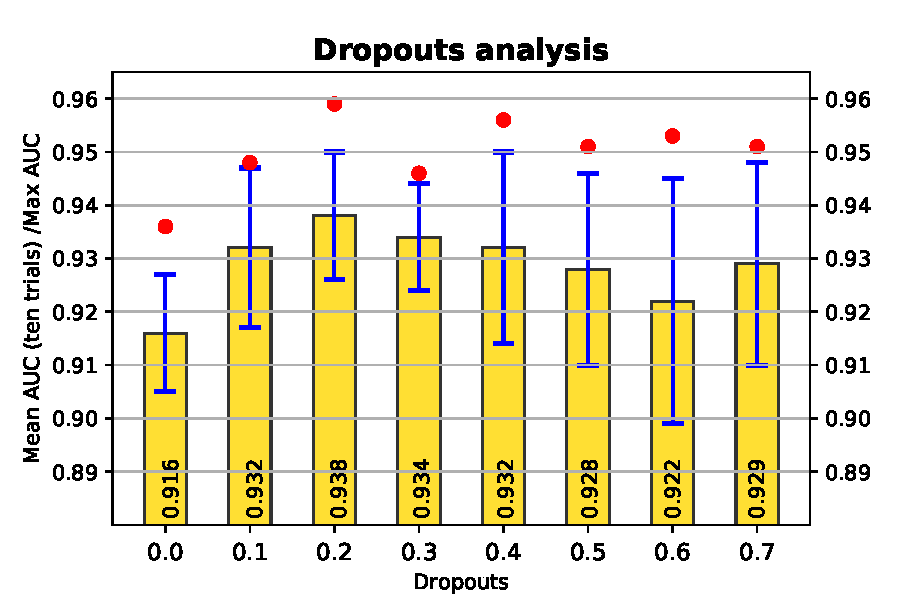
\includegraphics[width=7cm]{images/densenet/simple/densenet_simple_dropout}
\caption{DTC Dropout probability analysis}
\label{fig:densenet_simple_dropout}
\end{figure}

\paragraph{Discussion\\}
In figure \ref{fig:densenet_simple_dropout} it is observed that the 0.2 dropout configuration obtained the highest mean AUC. The other values with lesser dropout probability or greater dropouts are all gradually decreasing as they go further 
from the peak (0.2). With exception of the mean AUC obtained with 0.7 dropouts. The best value selected for further evaluation is 0.2.
%\flushbottom
%\newpage

\subsection{Batch Size Analysis}
For this analysis a limited search space is defined, with only batch size varies, the evaluation (10 trials for each test case) results are displayed in figure \ref{fig:densenet_simple_batchsize}.

\begin{figure}[ht]
\centering
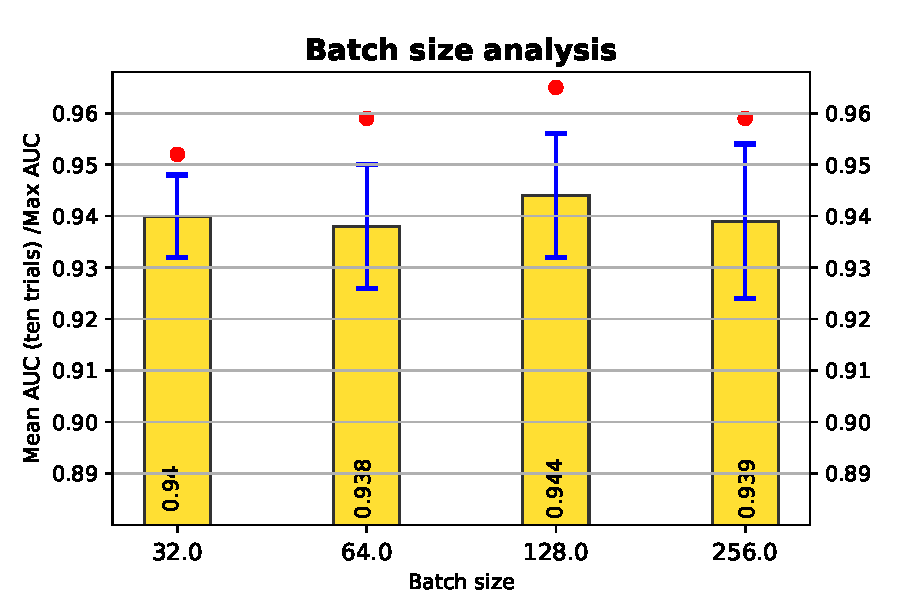
\includegraphics[width=6cm]{images/densenet/simple/densenet_simple_batchsize}
\caption{Batch size analysis}
\label{fig:densenet_simple_batchsize}
\end{figure}
 
\paragraph{Discussion\\}
From the figure \ref{fig:densenet_simple_batchsize} it is concluded that the batch size of 128 works the best. 
%\flushbottom
%\newpage

\subsection{Learning Rate and Optimizer Analysis}
For this analysis only Adadelta optimizer is used. This is based on the intuition that is formed during the DenseNet-Siamese evaluation.
But for the optimal learning rate the a series of discrete values are evaluated. The search space and results are presented in figure \ref{fig:densenet_simple_learning_rate}.
\begin{figure}[ht]
\centering
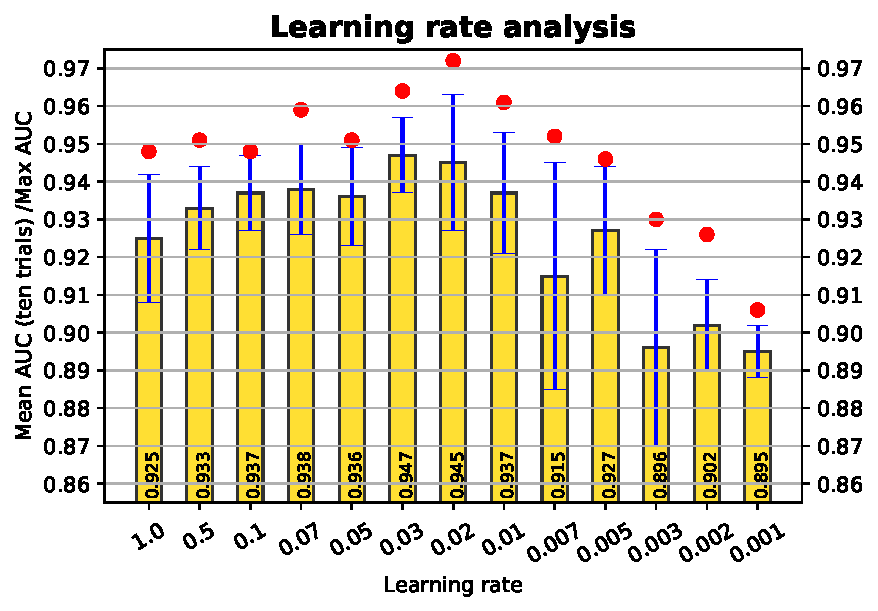
\includegraphics[width=10cm,height=6cm]{images/densenet/simple/densenet_simple_learning_rate}
\caption{Learning rate analysis}
\label{fig:densenet_simple_learning_rate}
\end{figure}

\paragraph{Discussion\\} 
From figure \ref{fig:densenet_simple_learning_rate} it is observed that the mean AUC with the learning rate 0.03 is slightly higher than the others. While one of the evaluation with 0.02 learning rate has 
obtained the maximum AUC of 0.972. But 0.03 is chosen as the best learning rate for further evaluations.


\subsection{DenseNet Two-Channel Final Grid Search}

\begin{table}[ht]
\centering
\caption{Best hyperparameter values for final evaluation of DenseNet two-channel.}
\resizebox{\textwidth}{!}
{\begin{tabular}{|l c| l c| l c|} 
 \hline\hline
 \rowcolor{lightgrey}
 \multicolumn{1}{|c}{\textbf{Name}} & \multicolumn{1}{c|}{\textbf{Value}} & \multicolumn{1}{c}{\textbf{Name}} & \multicolumn{1}{c|}{\textbf{Value}} \\ [0.5ex] 
 %Name & Value & Name & Value & Name & Value\\ [0.5ex] 
 \hline
 Layers & 2-2-2, 4-4-4, 6-6-6 & Pooling & 'avg'\\
 \hline
 Growth rate (gr) \& Number of filter & \multicolumn{3}{c|}{12 \& 32, 18 \& 32, 30 \& 8}\\
 
 \hline
 DenseNet dropout & 0.2 & Compression & 0, 0.5 \\ 
 \hline
 Bottleneck & 'False' & Batch size & 128 \\
 \hline
 Optimizer \& learning rate & \multicolumn{3}{c|}{'Adadelta' \& 0.03} \\
 \hline \hline
\end{tabular}}
\label{table:final_run_search_space_dtc}
\end{table}

%Growth rate, in the original paper, authors have mentioned that without bottleneck and compression the general trend is to use as high as possible growth rate. For the ImageNet, they have used growth rate 
 %up to 40. For all their experiments they have evaluated growth rates from 12 to 40. Since we do not have so much of data, we will evaluate the finer grid search with growth rates of 12(thin), 18 and 30(thick). 
Layers per block 2-2-2 it has very consistent performance in terms of mean AUC and also able to score high max AUC. It could have been possible to do architecture searches for 3 dense block architectures 
with layers per block close to 2-2-2, for example 2-3-3 etc. But then the search grid will be very big. Also included in the evaluation, layers 4-4-4 and 6-6-6. All other hyperparameters are displayed in the table
\ref{table:final_run_search_space_dtc}
 

The result is displayed in the table \ref{table:final_densenet_results}. unlike DenseNet-Siamese this final search space is much smaller and whole search space is visualized here in tabular format. Three architectures 2-2-2, 4-4-4 and 6-6-6 are 
evaluated for all three growth rates 12, 18, 30 and also for Reduction 0.5 and without Reduction. In the table \ref{table:final_densenet_results} the growth rate is displayed as Gr. and Reduction is displayed as R for space 
constraint.
\definecolor{Gray}{gray}{0.8}
\begin{center}
\begin{table}
 \caption{Final grid search results}
 \begin{tabular}{|c|l|cc|cc|cc|}\hline \hline
 \multirow{3}{*}{Gr.} & \multicolumn{1}{c|}{\multirow{3}{*}{Metrics}} & \multicolumn{6}{c|}{Layers per block} \\ \cline{3-8}
 & & \multicolumn{2}{c|}{2-2-2} & \multicolumn{2}{c|}{4-4-4} & \multicolumn{2}{c|}{6-6-6}\\ \cline{3-8}
 & & R=0 & R=0.5 & R=0 & R=0.5 & R=0 & R=0.5 \\ \hline \hline
 %\rowcolor{Gray}
 \multirow{4}{*}{12} & Mean AUC & \cellcolor{Gray}0.95 & \cellcolor{Gray}0.944 & \cellcolor{Gray}0.95 & \cellcolor{Gray}0.95 & \cellcolor{Gray}0.947 & \cellcolor{Gray}0.945 \\ %\cline{2-8}
  & Std & 0.011 & 0.015 & 0.009 & 0.01 & 0.008 & 0.008 \\ %\cline{2-8}
  & Max AUC & 0.97 & 0.97 & 0.963 & 0.965 & 0.963 & 0.955 \\ 
  & Total Parameters & 55,529 & 30,163 & 159,473 & 87,629 & 317,561 & 176,535 \\ \hline 
  %\rowcolor{Gray}
 \multirow{4}{*}{18} & Mean AUC & \cellcolor{Gray}0.952 & \cellcolor{Gray} 0.955 & \cellcolor{Gray} 0.951 & \cellcolor{Gray} 0.944 & \cellcolor{Gray} 0.948 & \cellcolor{Gray} 0.938 \\ %\cline{2-8}
  & Std & 0.008 & 0.009 & 0.005 & 0.011 & 0.006 & 0.014 \\ %\cline{2-8}
  & Max AUC & 0.967 & 0.966 & 0.956 & 0.963 & 0.956 & 0.955 \\ 
  & Total Parameters & 96,785 & 51,430 & 308,369 & 168,671 & 640,481 & 355,860 \\\hline 
  %\rowcolor{Gray}
 \multirow{4}{*}{30} & Mean AUC & \cellcolor{Gray} 0.943 & \cellcolor{Gray} 0.948 & \cellcolor{Gray} 0.943 & \cellcolor{Gray} 0.944 & \cellcolor{Gray} 0.932 & \cellcolor{Gray} 0.941 \\ %\cline{2-8}
  & Std & 0.008 & 0.008 & 0.01 & 0.013 & 0.015 & 0.011 \\ %\cline{2-8}
  & Max AUC & 0.959 & 0.964 & 0.96 & 0.962 & 0.948 & 0.953 \\ 
  & Total Parameters & 160,001 & 82,162 & 650,873 & 355,949 & 1,473,665 & 822,276 \\ \hline
 \hline
 \end{tabular}
\label{table:final_densenet_results}
\end{table}
\end{center}
\paragraph{Discussion\\}
The best result obtained has mean AUC of \textbf{0.955}. This is with reduction 0.5, 2-2-2 layers per block and growth rate of 18. Along with the other values mentioned in \ref{table:final_run_search_space_dtc} these are the best
hyperparameters for DenseNet two-channel, which might be specific to the dataset for the thesis. Normally it is observed that the 2-2-2 performance
is very similar to that of 4-4-4, in fact slightly better. The performance of 6-6-6 is bit worse than the other too. 
Although, because of reduction the auc is observed to be slightly lower some times, some times it is higher than the without reduction result. But the size of the total parameters 
of the network with Reduction(R)=0.5 is always close to half size of the equivalent network without Reduction. So that is always beneficial as it is less computationally expensive.
In Valdenegro-Toro \cite{stateoftheart} work it is also found that the simple two-channel network better than the Siamese network. By comparing DenseNet two-channel and DenseNet-Siamese same trend is observed.

During the hyperparameter search many high accuracy network models are recorded, the highest AUC recorded for any of the DenseNet two-channel is 0.972, which is found with 'basic network' structure and learning rate 0.02. 
The ROC for the prediction is displayed in figure \ref{fig:densenet_two_channel_ninetysevenAUC}.
\begin{figure}[ht]
\centering
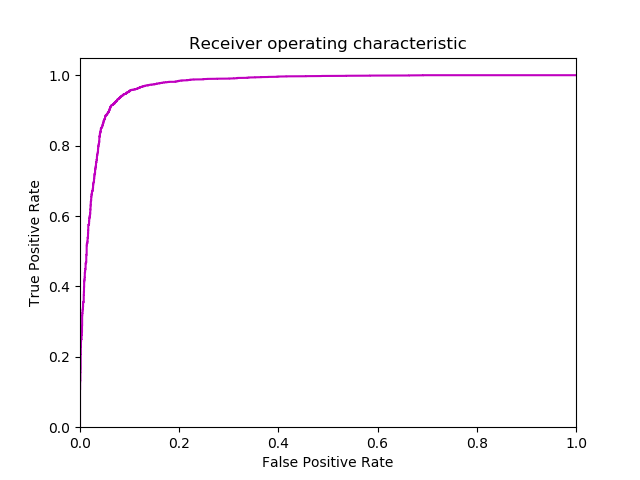
\includegraphics[height= 5cm]{images/densenet/densenet_two_channel_ninetysevenAUC}
\caption{Overall best result for DenseNet two-channel 0.972 AUC (Single run)}
\label{fig:densenet_two_channel_ninetysevenAUC}
\end{figure}

\subsubsection{Top 6 Configurations}
Instead of top 5, top 6 configurations are mentioned here, because the 6th one has same mean AUC and 4th and 5th. Table \ref{table:final_run_search_space_dtc} contains the overall search space for this search. Those parameters which has 
multiple values in the search space, best values for those are mentioned table \ref{table:dtc_final_run_best_configs}, e.g. reduction, 0 and 0.5.
In table \ref{table:dtc_final_run_best_configs} the \code{'Config alias'} are the aliases for the configurations, for future reference.

\begin{table}[ht]
\centering
\caption[Best hyperparameter values for the DenseNet two-channel ...]{Best hyperparameter values for the DenseNet two-channel, obtained from the final grid search. In decreasing order of their mean prediction accuracy on the test data. 
Top 6 results are mentioned.}
\resizebox{\textwidth}{!}
{\begin{tabular}{|l l c c c c c c|} 
 \hline\hline
 \rowcolor{lightgrey}
\textbf{Config alias} & \textbf{Layers} & \textbf{Growth rate} & \textbf{Epochs} & \textbf{Compression} & \textbf{Mean AUC} & \textbf{Std} & \textbf{Max AUC}\\
\hline
'Config 1' & 2-2-2 & 18 & '21' & 0.5 & 0.955 & 0.009 & 0.966 \\
'Config 2' & 2-2-2 & 18 & '25' & 0 & 0.952 & 0.008 & 0.967 \\
'Config 3' & 4-4-4 & 18 & '21' & 0 & 0.951 & 0.005 & 0.956  \\
'Config 4' & 2-2-2 & 12 & '23' & 0 & 0.95 & 0.011 & 0.97 \\
'Config 5' & 4-4-4 & 12 & '21' & 0 & 0.95 & 0.009 & 0.963  \\
'Config 6' & 4-4-4 & 12 & '21' & 0.5 & 0.95 & 0.01 & 0.965  \\
\hline \hline
\end{tabular}}
\label{table:dtc_final_run_best_configs}
\end{table}

\begin{figure}[ht]
\centering
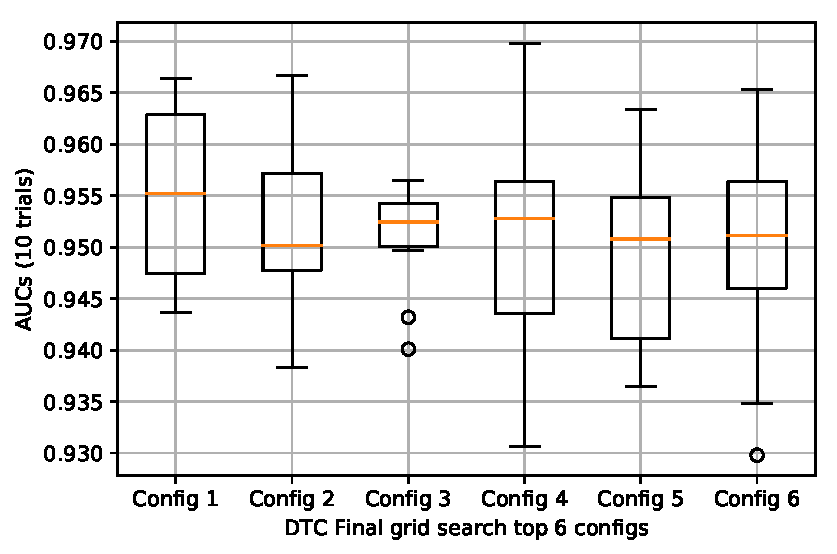
\includegraphics[width=10cm]{images/densenet/simple/top_config_boxplot}
\caption{Boxplot analysis for top configurations, with statistical outlook on 10 AUC scores obtained for each cases.}
\label{fig:top_config_boxplot_dtc}
\end{figure}

\paragraph{Discussion\\}
From the boxplot \ref{fig:top_config_boxplot_dtc}, how the 10 prediction values on test data are distributed are evaluated, with a statistical outlook. For example the distribution for third and second configuration are very condensed, i.e 
less standard deviation, which is also supported from the data in table \ref{table:dtc_final_run_best_configs}. Two of the configurations display outliers, which means those readings are much wider in comparison to other readings. But the 
'Config 2', which has overall second highest average AUC, has the lowest median. This signifies most data points are actually lower than the mean of the distribution, just few high auc scores pulled up the overall average.
So with respect to median it is the worst configuration among the 6. From table \ref{table:dtc_final_run_best_configs} it is observed that growth rate 18 is the best performer, followed by 12, while only two out of six
entries are using compression. 2-2-2 is best performing network, but 4-4-4 is also very close. Even the median for 'Config 1' is highest, along with highest mean AUC, this is the overall best DenseNet two-channel configuration.


\flushbottom
\newpage

\section{VGG-Siamese Network with Contrastive Loss}
\label{sec:contrastive_loss_results}
In this section, important hyperparameters of VGG-Siamese network with contrastive loss are listed and the grid search result is presented with help of visualizations. At the end, the optimized prediction result with best hyperparameter 
values obtained from the grid search is also presented. %TODO either link the existing image or make another wrap figure or something here

\subsection{Hyperparameters To Be Evaluated}

The hyperparameters can be divided into two types, VGG branch related and other general hyperparameters. In Siamese part the distance is computed directly from the output of the branches. As decision, the network outputs the computed distance
between the input patches, so the decision network of the Siamese does not have any hyperparameters.
Each VGG branch has the architecture as follows: \\ \code{Conv(n, a x a)-Conv(n, a x a)-MP(2, 2)-Conv(2n, a x a)-Conv(2n, \\a x a)-MP(2, 2)-
Conv(4n, a x a)-Conv(4n, a x a)-Conv(4n, a x a)-\\MP(2, 2)-Conv(8n, a x a)-Conv(8n, a x a)-Conv(8n, a x a)-MP(2, 2)-\\Conv(8n, a x a)-Conv(8n, a x a)-Conv(8n, a x a)-MP(2, 2)-FC(d)}. \\There could be up to 3 FC layers at the end, denoted by l.
Also there could be batch normalization layers after all the FC layers in VGG branch. %The batch normalization layer could be placed before the activation ReLU layer or after. 
Variables n, a, l, d are the hyperparameters of the VGG branches. The overall search space for the hyperparameters are displayed in the table \ref{table:Search_space_contrastive}.

\begin{table}[ht]
\centering
\caption{The search space for VGG-Siamese network with Contrastive loss.}
\resizebox{\textwidth}{!}
{\begin{tabular}{|l c| l c|} 
 \hline\hline
 \rowcolor{lightgrey}
 \multicolumn{1}{|c}{\textbf{Name}} & \multicolumn{1}{c|}{\textbf{Value}} & \multicolumn{1}{c}{\textbf{Name}} & \multicolumn{1}{c|}{\textbf{Value}} \\ [0.5ex] 
 \hline
 Conv filters & 8, 16, 32, 64 & Kernel size & 3, 5, 7\\
 \hline
 FC Layers & 1, 2, 3 &  FC output & 32, 64, 96, 256, 512, 1024, 2048 \\ 
 \hline
 Batch normalization & True, False & Dropout & 0.1, 0.2, 0.3, 0.4, 0.5, 0.6, 0.7 \\
 \hline
 Batch size & 32, 64, 128, 256, 512 & Optimizer & Adam, Nadam, Adadelta, Adamax, RMSprop\\
 \hline
 Initializers & \multicolumn{3}{c|}{ He\_normal, He\_uniform, Glorot\_uniform, Glorot\_normal, RandomNormal} \\
 \hline
 Learning rates & \multicolumn{3}{c|}{0.01, 0.007, 0.005, 0.002, 0.0007, 0.0005, 0.0002, 0.0001, 0.00007, 0.00005, 0.00002, 0.00001}\\
 \hline \hline
\end{tabular}}
\label{table:Search_space_contrastive}
\end{table}

Overall search space is divided into smaller parts and evaluated with a common basic network structure, that gives good prediction accuracy already. The Basic network structure is obtained after manual tuning and many trials.

\subsection{Basic Network Structure}
This network structure is used for all the focused hyperparameter search. Keeping other values same, only changing the values for the targeted and related parameters, should help building an intuition of how the network behaves 
with different values of the targeted parameter and should help in selecting the best value from the predefined search space.

\begin{table}
 \centering
\caption{Basic network configuration for the hyperparameter search. In this section of report this configuration will be referred to by the alias of 'basic network structure'.}
\resizebox{\textwidth}{!}
{\begin{tabular}{|c | c| c| c| c|} 
\hline\hline
 \rowcolor{lightgrey}
 Conv filters & Kernel size & FC Layers & FC output & Batch normalization \\ 
  16 & 3 & 1 & 128 & FALSE\\ 
 \hline
 \rowcolor{lightgrey}
 Dropout & Batch size & Optimizer & Initializers & Learning rates\\[0.5ex]
 \hline
 0.2 & 64 & adam & random normal(Conv) + He normal(FC) & 0.00001\\[0.5ex]
 \hline \hline
\end{tabular}}
\label{table:basic_vgg_network}
\end{table}

\subsection{Flipped Labels}
Since contrastive loss returns projected distance, here close to zero means similarity and 1 means dissimilarity. Although, in our original data label 1 represents similarity between patches.
Hence the labels for train, validation and test data here are all flipped. Operation \code{new\_label = 1 - old\_label} is applied to all three data labels. So for this evaluation input label 0 means similarity between patches.

\subsection{Conv Filters Analysis}
The \code{filters} \cite{kerasconv} defines the number of output filters in each convolution layers. Now for all the 13 convolution layers in the network the filters size can be easily calculated from the first filter size. In previous section
it has been shown that the filters for the Conv layers are n, n, 2n, 2n, 4n, 4n, 4n, 8n, 8n, 8n, 8n, 8n, 8n respectively. Here 4n means 4 times n. So for each value of filters (n) in the search space [8, 16, 32, 64], the filter values
are computed for all 13 Conv layers and each configuration is evaluated 10 times. Evaluation results are displayed in the figure \ref{fig:contrastive_loss_con2d_filter_bar}.

\begin{figure}[ht]
\centering
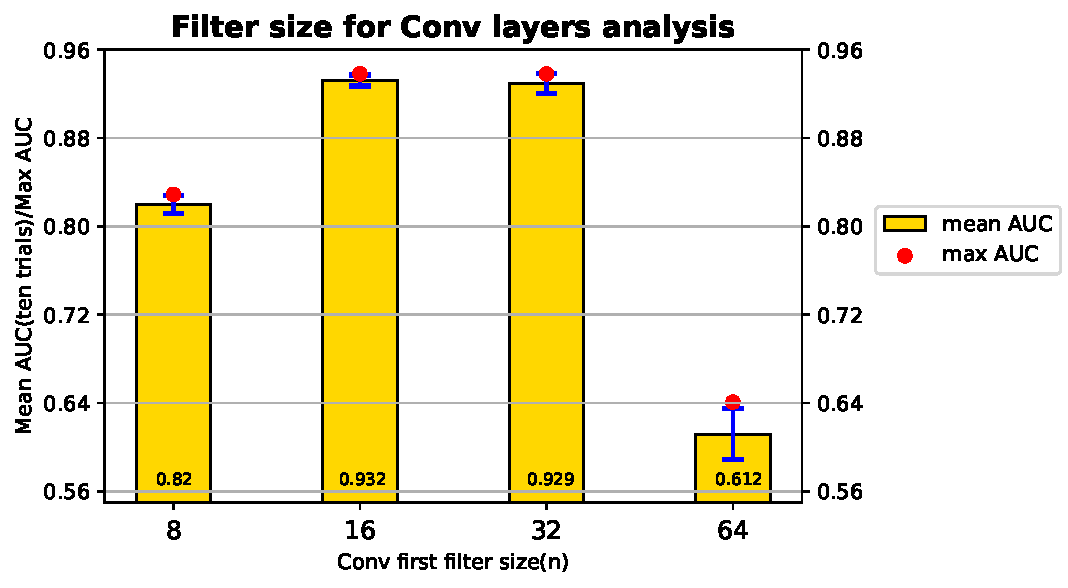
\includegraphics[width=10cm,height=5cm]{images/contrastive/contrastive_loss_con2d_filter_bar}
\caption{Conv filters size analysis for VGG branches.}
\label{fig:contrastive_loss_con2d_filter_bar}
\end{figure}

\paragraph{Discussion\\}
From figure \ref{fig:contrastive_loss_con2d_filter_bar} the highest mean AUC is for 16. So for the best performing network is having the VGG branch with filters for the convolution layers as follows, 
16, 16, 32, 32, 64, 64, 64, 128, 128, 128, 128, 128, 128. The performance for filter size 32 is also very good, but 16 is selected as the best value.

\subsection{Kernel Size Analysis}
The kernel size parameter defines the height and width of the 2 dimensional convolution window for all the Conv layers in the VGG network. From table \ref{table:kernel_size} it is clear that with kernel size 3 
network learns much better than 5 and 7 kernel sizes. 

\begin{center}
  \begin{tabular}{|c c c|} 
   \hline\hline
   \rowcolor{lightgrey}
   Rank & Kernel size & Mean AUC (10 trials) \\[0.5ex] 
   \hline
   1 & 3 & 0.932\\   
   \hline
   2 & 5 & 0.799\\   
   \hline
   3 & 7 & 0.481\\   
   \hline \hline
  \end{tabular}
 %\caption{Kernel size analysis}
 \label{table:kernel_size}
\end{center}

\subsection{FC Units Size Analysis} 
The hyperparameter FC output, also known as units in Keras, denoted by (d), determines the output size of the layer. For each values of (d) from the search space of [64, 96, 128, 256, 512, 1024, 2048], one, two and three FC(d) 
layers along with ReLU activations are added at the end of each VGG branch. Ten trials are done for each of the configuration.  
So the goal of this grid search is to find the best values of d and l. The search results are displayed in the figure \ref{fig:contrastive_loss_dense_bar}.

\begin{figure}[ht]
\centering
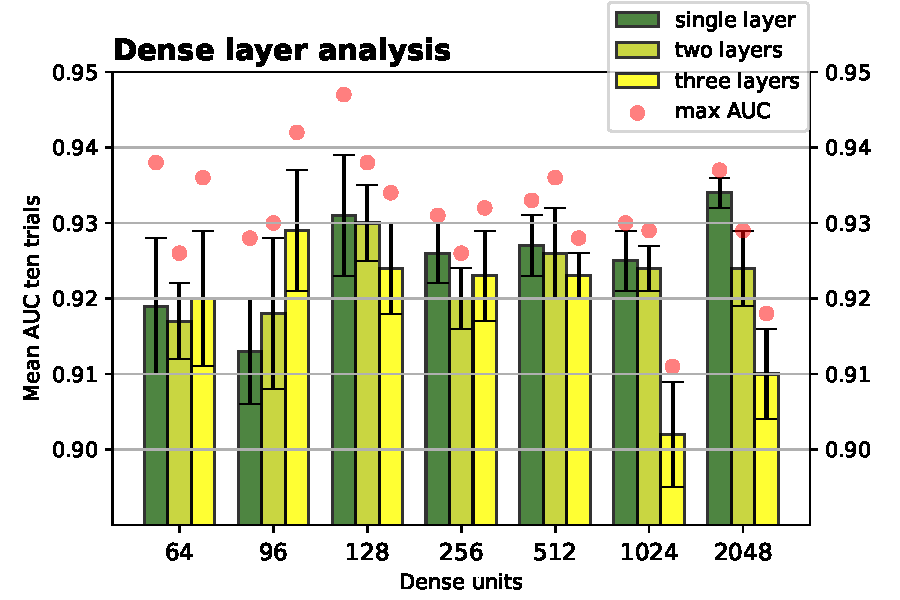
\includegraphics[width= 13cm,height=6cm]{images/contrastive/contrastive_loss_dense_bar}
\caption{FC units and layers analysis for VGG branches.}
\label{fig:contrastive_loss_dense_bar}
\end{figure}

\paragraph{Discussion\\}
From \ref{fig:contrastive_loss_dense_bar} single FC layer (l=1) in figure works best. Although performance of two FC layers (l=2) are also very close, single layers are selected as best values. Just for validation,
the best configuration of the final grid search can also be verified for two layer structures.
128 and 2048 has been selected for the final grid search as they have the highest mean AUCs. Although this is bit unexpected to see two points close to the opposite extremes of search space to yield best results.

%\flushbottom
%\newpage

\subsection{Initializers}
Keras initializers \cite{kerasinit} control or define the way the initial random weights in keras layers are set.
In the following part the brief introduction of the initializers and how they can be instantiated in Keras is presented. These definitions and instantiation examples are taken from official Keras \cite{kerasinit} documentation.

\begin{enumerate}
 \item \textbf{Zeros} : This is one of the simplest of the initializers. It generates tensors initialized to 0. In Tensorflow, tensors are represented by n-dimensional arrays of base data type.\\
Instantiation: \code{keras.initializers.Zeros()}
 \item \textbf{RandomNormal} : This initializer uses normal distribution to initialize generated tensors.\\
Instantiation: \code{keras.initializers.RandomNormal(mean=0.0, stddev=\\0.05,seed=None)}
\item \textbf{RandomUniform} : This initializer uses uniform distribution to initialize generated tensors.\\
Instantiation: \code{keras.initializers.RandomUniform(minval=-0.05,}\\
 \code{maxval=0.05, seed=None)}
 \item \textbf{Glorot\_normal} : Glorot normal initializer is also known as Xavier normal initializer. It generates samples from a truncated normal distribution which is centered at 0 with 
standard deviation of \code{(stddev) = sqrt(2 / (fan\_in + fan\_out))}. \code{fan\_in} represents number of input units in the weight tensor. The number of output units in the weight tensor is denoted by \code{fan\_out}.\\
Instantiation: \code{keras.initializers.glorot\_normal(seed=None)}
 \item \textbf{Glorot\_uniform} : Glorot uniform initializer is also called Xavier uniform initializer. It draws samples from a uniform distribution within [-limit, limit] 
where limit is \code{sqrt(6 / (fan\_in + fan\_out))}, \code{fan\_in} represents number of input units in the weight tensor. The number of output units in the weight tensor is the \code{fan\_out}.\\
Instantiation: \code{keras.initializers.glorot\_uniform(seed=None)}
 \item \textbf{He\_normal} : It draws samples from a truncated normal distribution centered on 0 with standard deviation \code{(stddev) = sqrt(2 / fan\_in)} where \code{fan\_in} represents the number of 
input units in the weight tensor.\\
Instantiation: \code{keras.initializers.he\_normal(seed=None)}
 \item \textbf{He\_uniform} : He uniform variance scaling initializer draws samples from a uniform distribution within [-limit, limit]. Here, limit is \code{sqrt(6 / fan\_in)} and \code{fan\_in} represents the number
of input units to the weight tensor.\\
Instantiation: \code{keras.initializers.he\_uniform(seed=None)}
\end{enumerate}

Kernel initializers for the convolution layers and kernel initializers for the FC layers are investigated here. The search space for kernel initializers for convolution layers (Conv) contains [He normal
and uniform, Glorot normal and uniform and random normal]. These initializers are selected after some manual trials. With random uniform (default Instantiation) as Conv initializer, the 
network fails to converge. Hence it is not evaluated. The search space for initializers for FC layer contains [He normal and uniform and Glorot normal and uniform]. The bias initializer, for both Conv and FC layers, 
is left with the default \code{Zeros} initializer.
In keras, for both Conv and FC the default kernel initializer is Glorot uniform. Popular intuition is that Glorot or Xavier initialization works better with Sigmoid activation, while He uniform/normal works better with ReLU. %TODO cite source
 In the network architecture there are 13 Conv layers compared to only one or two FC layer/s, so the Conv initializer is expected to have more effect.
All the initializers used with default instantiation. 
%add sources/references

\begin{figure}[ht]
\centering
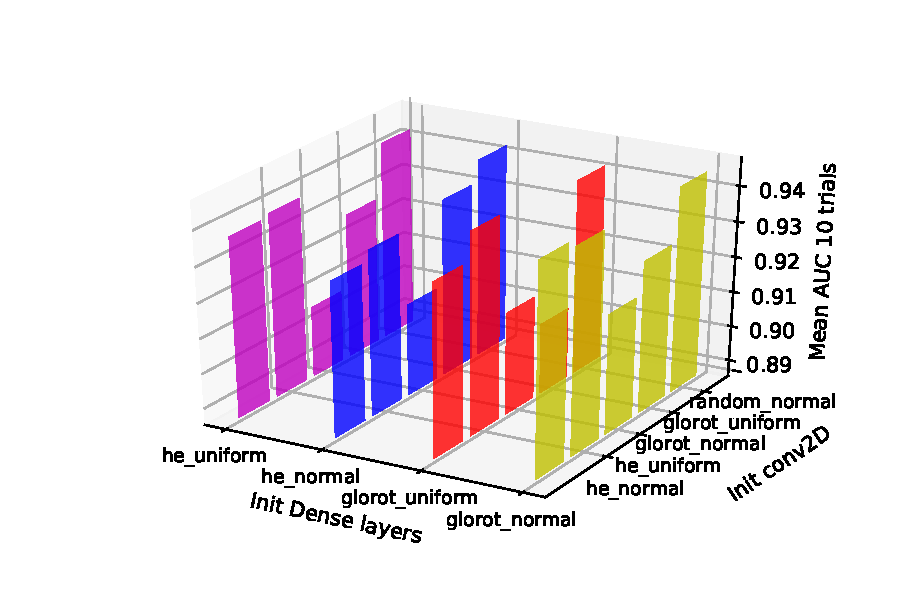
\includegraphics[height= 8cm]{images/contrastive/3DbarGraph}
\caption[Performance comparison of different combinations of Conv and FC initializers]{Performance comparison of combinations for Conv and FC layer initializers, in one axis the initializers for FC or Dense layers are displayed in unique colors, in the other axis the initializers for Conv layers are showed. Z-axis or 
height of the bars represents the mean AUC in ten trials obtained for each combination of Conv and FC initializers.}
\label{fig:3DbarGraph_initialization}
\end{figure}

\paragraph{Discussion\\}
In this figure \ref{fig:3DbarGraph_initialization}, observed mean AUC is reported for different combinations of Conv initializer and FC Initializer. The x-axis of the graph represents FC layer initializer 
and the y axis represents the Conv initializer. In the z axis the mean AUC of ten trials is shown. The z-axis values are clipped and starts from 0.89. This is 
to be able to show the differences in values (bar heights) effectively. Otherwise, if the bars are plotted from zeros the difference is hard to perceive as the values are very close.
Lowest mean AUC value obtained is 0.903 and the highest is 0.943. The bar chart starting value selected in such a way that all the bars are visible and comparable.

The performance of random normal as the initializer for Conv layers is over all good. Performance of the Glorot normal and uniform as Conv initializer is comparatively worse than others.
Performance of both He initializers are over all good as Conv initializer. 
As the FC layer initializer glorot normal is found to have performed the best.
Over all performance wise the combination of He normal as the Conv and glorot normal as the FC initializer, have yielded highest mean AUC (0.943 AUC). The results for top 6 combinations are presented in table \ref{table:kernel_init} in descending
order of the yielded mean AUC. 

\begin{center}
 \begin{table}
  \begin{tabular}{|c l l c c c|} 
   \hline\hline
   \rowcolor{lightgrey}
   Rank & Init Conv & Init FC & Mean AUC & STD & MAX AUC\\ [0.5ex] 
   \hline
   1 & He normal & Glorot normal & 0.943 & 0.007 & 0.953 \\ 
   \hline
   2 & He uniform & Glorot normal & 0.941 & 0.012 & 0.961 \\
   \hline
   3 & Random normal & Glorot normal & 0.941 & 0.004 & 0.946 \\
   \hline
   4 & He uniform & Glorot uniform & 0.94 & 0.008 & 0.952\\
   \hline
   5 & Random normal & He normal & 0.939 & 0.005 & 0.946\\
   \hline
   6 & Random normal & He uniform & 0.939 & 0.005 & 0.948\\
   \hline \hline
  \end{tabular}
 \caption{Kernel initializer top results}
 \label{table:kernel_init}
\end{table} 
\end{center}
A strong trend is observed with random normal Conv initializers, the standard deviation for it is very low, though the maximum AUC values are consistently lower than the He variations. Glorot normal works very consistently as initializer for 
FC layers. Therefore it is selected as the FC initializer. But there is no clear winner for Conv initializers, so both He and random normal initializers are selected for the final grid search. 

\subsection{Batch Normalization Analysis}
Small batch training is better than one by one training and it is also better than
training the whole dataset at once. Small batch training with batch normalization is advantageous because it converges faster than doing one by one. Batch normalization reduces the need for carefully tuning the 
initial weights, also to some extend limits the need for too much of regularizers such as dropouts. Concept of batch normalization is introduced by Ioffe and Szegedy in 2015 \cite{ioffe2015batch}. 
The authors are influenced by the idea from Lecun,1998b \cite{lecun1998gradient} and Wiesler and Ney, 2011 \cite{wiesler2011convergence} that if inputs to a CNN are linearly transformed to have unit 
variance and zero mean, then the network will converge faster. The learning rates are generally kept comparatively lower because 
an outlier might cause big effect in already learned activations. As a result of keeping the inputs normalized the outlier cases also affects the overall learning process lesser. Hence batch normalization
should also enable the use of higher learning rates. The batch normalization layer is usually applied after each fully-connected or dense layer, apart from the output. In this thesis, the batch normalization is evaluated three steps,
firstly, without batch normalization. 
Then, with batch normalization, when adding the batch normalization layer after the dense layer but before the activation function 'ReLU'. Thirdly, after both, dense layer and activation 'ReLU'. Mean AUC comparisons are as follows
(same epochs).

\begin{table}[ht]
 \centering
  \caption{Batch normalization analysis for VGG branches.}
  \begin{tabular}{|c c c c c|} 
   \hline\hline
   \rowcolor{lightgrey}
   Rank & Batch normalization & Mean AUC (10 trials) & STD & Max AUC\\[0.5ex] 
   \hline
   1 & Without & 0.932 & 0.005 & 0.938\\   
   \hline
   2 & Before activation ReLU & 0.9 & 0.012 & 0.926\\  
   \hline
   3 & After activation ReLU & 0.874 & 0.011 & 0.893\\  
   \hline \hline
  \end{tabular}
 \label{table:batch_normalization_contrastive}
\end{table}

The results from \ref{table:batch_normalization_contrastive} are bit surprising. It is noted that with batch normalization during the training the network can achieve higher training accuracy in the same number of epoch than without batch normalization. 
However the generalization performance on the test data is worse using batch normalization. With batch normalization cases are also tested for lesser and greater epochs than without batch normalization, it still scores poorer results.

\begin{figure}[ht]
\centering
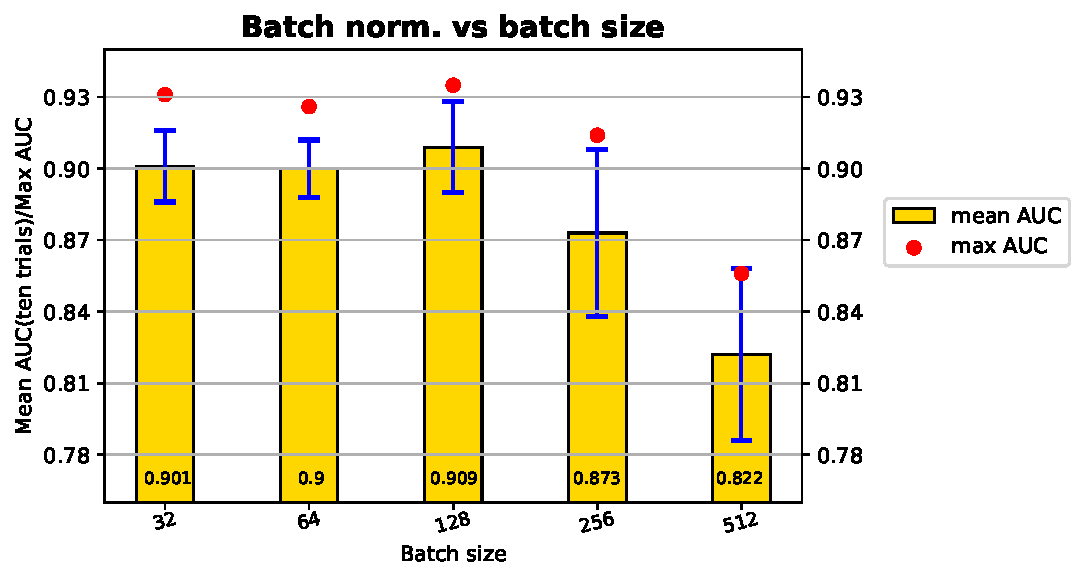
\includegraphics[width=10cm,height= 5.5cm]{images/contrastive/contrastive_loss_bnvsbs_bar}
\caption{Evaluation of how batch normalization affects prediction with increase in batch size.}
\label{fig:contrastive_loss_bnvsbs_bar}
\end{figure}

The batch size and batch normalization correlation analysis is done in figure \ref{fig:contrastive_loss_bnvsbs_bar}. The idea is that the batch normalization performance might increase with increase in the batch size. The 
bigger the batch size is, the more it resemble the actual distribution that represents the whole data, this is one of the intuition. No strong evidence are found in this direction, though the mean AUC slightly peaked from 
batch size 32 to 128 and then sharply fell down.

Since batch normalization limits the effect of outliers, could it be the case that the apparent outliers contained discriminative features somehow. Because of sonar images 
have low signal to noise ratio, it could be that the perceived noise is actually useful data, which get somewhat filtered out by the batch normalization. However this is only speculation, no concrete analysis is done in this 
direction. But batch normalization layers are not used for further evaluation.

\subsection{Dropout Probability Analysis}

\begin{figure}[ht]
\centering
\includegraphics[width= 12cm,height= 7cm]{images/contrastive/contrastive_loss_dropout_bar}
\caption{Dropouts probability analysis for VGG branches.}
\label{fig:contrastive_loss_dropout_bar}
\end{figure}

From the figure \ref{fig:contrastive_loss_dropout_bar} it is noticeable that the performance (mean AUC across 10 trials) for dropout values 0.3, 0.4, 0.5 and 0.6 are very close. 
The network achieved highest mean AUC with dropout probability 0.4 and 0.6, so they are chosen as the best values. With those values network performed better than dropout 0 and 0.1, which offers too less regularization leading to overfit. 
Also performed better than 0.7 dropout which provides too much regularization. This is a expected result, and matches on the common experience.

\subsection{Learning Rate And Optimizer}
The search space for optimizer contains Adam, Nadam, Adamax, RMSprop, Adadelta. For the learning rate, evaluation started with learning rate search space as [0.007, 0.005, 0.002, 0.001, 0.0007, 0.0005, 0.0002, 0.0001, 0.00007, 0.00005, 0.00002, 0.00001]
for all the optimizers. It is noticed that the network, for all optimizers, does not train for all the learning rates. Finally, learning rates for each optimizer is selected individually. The search space is displayed below in table 
\ref{table:search_space_lr_contrastive}.

\begin{table}[ht]
 \centering
 \caption{The search space for learning rates specific for each optimizer for VGG-Siamese and Contrastive loss network.}
 \begin{tabular}{|c| c|} 
 \hline\hline 
 \rowcolor{lightgrey}
 %\hline
 Adamax & Adadelta\\ [0.5ex] 
 \hline
 0.001, 0.002, 0.005, 0.007 & 0.1, 0.2, 0.5, 0.7, 1.0 \\
 0.0001, 0.0002, 0.0005, 0.0007 & 0.01, 0.02, 0.05, 0.07\\
 0.00001, 0.00002, 0.00005, 0.00007 & 0.005, 0.007\\
 \hline
 \rowcolor{lightgrey}
 \multicolumn{2}{|c|}{Adam, Nadam and RMSprop} \\[0.5ex] 
 \hline
 \multicolumn{2}{|c|}{0.0001, 0.0002, 0.0005}\\
 \multicolumn{2}{|c|}{0.00001, 0.00002, 0.00005, 0.00007}\\
 \hline \hline
\end{tabular}
\label{table:search_space_lr_contrastive}
\end{table}

\begin{figure}[ht]
\centering
\includegraphics[width=10cm,height= 6cm]{images/contrastive/contrastive_loss_optimizer_bar}
\caption{Search results of best optimizer and learning rate}
\label{fig:contrastive_loss_optimizer_bar}
\end{figure}

\paragraph{Discussion\\} 
Ten trials per test cases are done. The learning rate for which each optimizer obtained best mean AUC result, are compared and visualized in figure \ref{fig:contrastive_loss_optimizer_bar}, it is noted that the best mean AUC for all the 
optimizers are very good, though for different learning rates. 
For each optimizer the best learning rates are as follows: Adam-0.00001, Nadam-0.0002, Adadelta-0.005, Adamax-0.0007, RMSprop-0.0002. Nadam is the best performer.
From figure \ref{fig:contrastive_loss_optimizer_bar} network with Nadam has highest mean AUC and highest max AUC both. So Nadam optimizer and starting learning rate 0.0002 is selected for the final grid search.

\subsection{Batch Size Analysis}
To find the best optimal batch size, a search space containing [32, 64, 128 and 256] is evaluated.

\begin{figure}[ht]
\centering
\includegraphics[width=10cm,height= 5.5cm]{images/contrastive/contrastive_loss_batchsize_bar}
\caption{Batch size analysis}
\label{fig:contrastive_loss_batchsize_bar}
\end{figure}

It is observed from figure \ref{fig:contrastive_loss_batchsize_bar} that the test AUC somehow increases with the increase in batch size, and opposite to expectation, takes more epochs to reach the convergence. 
Since the 256 batch size is at the boundary of search space, which performed the best, batch size 512 is also evaluated. But it does not train well and the validation accuracy remains stuck near 50\%.
hence batch size 256 is chosen for the final evaluation. 

\subsection{Total Parameter Analysis}
For determining how well a network work, it is important to find out the total parameter size. For the 'basic network structure' with FC output size 2048 and single FC layer, the total parameters are 3281840. 
But for network with FC output size 128 has only 1068080 total parameters. FC output size is the main hyperparameter which control the total parameter size for this network.

\subsection{Final Grid Search}
All the best performing hyper parameter values are configured together for this final run. The overall prediction accuracy for the network should be improved with these optimized hyperparameter values.
The search space for the final grid search is displayed below in table \ref{table:final_search_space_contrastive}.
 
\begin{table}
 \centering
\caption[Final grid search space VGG-Siamese network.]{The search space for final grid search for the VGG-Siamese network with Contrastive loss.}
\resizebox{\textwidth}{!}
{\begin{tabular}{|c | c| c| c| c|} 
\hline\hline
 \rowcolor{lightgrey}
 Conv filters & Kernel size & FC Layers & FC output & Batch normalization \\ 
  16 & 3 & 1 & 128, 2048 & FALSE\\ 
 \hline
 \rowcolor{lightgrey}
 Dropout & Batch size & Optimizer & Initializers & Learning rate\\[0.5ex]
 \hline
 &&& random normal(Conv) + glorot normal(FC) & \\[0.5ex]
 0.4, 0.6 & 256 & Nadam & he uniform(Conv) + glorot normal(FC) &  0.0002\\
 &&& he normal(Conv) + glorot normal(FC) & \\
 \hline \hline
\end{tabular}}
\label{table:final_search_space_contrastive}
\end{table} 

Ten evaluations are done for each of the test cases, training the network from scratch every time, which is a good test-scenario for the initializers evaluation. The results are displayed in the figure \ref{fig:contrastive_loss_final_bar}.
The sub-figure \ref{fig:contrastive_loss_final_04_bar} presents the comparative view of the result obtained by the network with all combination of configurations mentioned in \ref{table:final_search_space_contrastive}, for dropout value 0.4.
Similarly for dropout value 0.6 is displayed in the \ref{fig:contrastive_loss_final_06_bar}.

\begin{figure}
  \centering
  \begin{subfigure}[b]{5.885cm}
    \includegraphics[width=\textwidth]{images/contrastive/contrastive_loss_final_04_bar}
    \caption{Comparative analysis of the final grid search for dropout 0.4.}
    \label{fig:contrastive_loss_final_04_bar}
  \end{subfigure}
  ~ %add desired spacing between images, e. g. ~, \quad, \qquad, \hfill etc. 
   %(or a blank line to force the subfigure onto a new line)
  \begin{subfigure}[b]{7cm}
    \includegraphics[width=\textwidth]{images/contrastive/contrastive_loss_final_06_bar}
    \caption{Comparative analysis of the final grid search for dropout 0.6.}
    \label{fig:contrastive_loss_final_06_bar}
  \end{subfigure}    
  \caption[Final grid search results for VGG-Siamese network with Contrastive loss.]{Final grid search results for VGG-Siamese network with Contrastive loss. The result for whole search space is visualized here, which is divided
  in two figures for dropout values 0.4 and 0.6.}
  \label{fig:contrastive_loss_final_bar}
\end{figure}

\paragraph{Discussion\\}
In figure \ref{fig:contrastive_loss_final_bar} in each sub-figure x-axis contains the initializer combinations for Conv and FC layer. For each combination of initializers, two bars are plotted representing mean AUC,
obtained for each of the 128 and 2048 FC units value. Y-axis represents mean AUC in ten trials and maximum AUC. The y-axis scales for both sub-figures are matched so that they can be visually compared.
The best result for dropout 0.4 is mean AUC (Ten trials) of 0.944 with std of 0.007 and highest AUC value in a single run as 0.95. The best
result for dropout 0.6 is mean AUC (Ten trials) of 0.949 with std of 0.005 and highest AUC value in a single run as 0.956. Both aforementioned networks has random normal and glorot normal as Conv and FC layer initializers respectively,
this combination is clearly best suited for the dataset. Also in both cases the FC output size is 2048. Overall highest mean AUC for the VGG-Siamese network with Contrastive loss is 0.949, which is clearly improvement over the
state of the art result of 0.894 AUC for score prediction on the same test dataset.

% In addition to the hyperparameters, which has best values already determined, presented in table \ref{table:final_search_space_contrastive}, FC output, dropout and initializers best values are as follows: 2048, 0.6 and random normal (Conv), 
% glorot normal (FC).
The ROC for the network which yielded maximum AUC for the best configuration, with score of AUC 0.956, is presented in figure \ref{fig:keras_contrastive_loss_20Dec2pm0}
\begin{figure}[ht]
\centering
\includegraphics[height= 5cm]{images/contrastive/keras_contrastive_loss_20Dec2pm0_956}
\caption{ROC for the highest auc recorded for the network with best configuration.}
\label{fig:keras_contrastive_loss_20Dec2pm0}
\end{figure}

In addition to the hyperparameters, which has best values already determined, presented in table \ref{table:final_search_space_contrastive}, rest of the parameter values for the top 4 configurations are displayed in 
\ref{table:contrastive_final_run_best_configs}. The configurations are ordered according to decreasing order for the mean AUC.
\begin{table}[ht]
\centering
\caption[Best hyperparameter values for the Vgg-Siamese with contrastive loss ...]{Best hyperparameter values for the Vgg-Siamese with contrastive loss, obtained from the final grid search. In decreasing order of their mean 
prediction accuracy on the test data. Top 4 results are mentioned.}
\resizebox{\textwidth}{!}
{\begin{tabular}{|l c c l l c c c|} 
 \hline\hline
 \rowcolor{lightgrey}
\textbf{Config alias} & \textbf{FC output} & \textbf{Dropout probability} & \textbf{Conv initializer} & \textbf{FC initializer} & \textbf{Mean AUC} & \textbf{Std} & \textbf{Max AUC}\\
\hline
'Config 1' & 2048 & 0.6 & random normal & glorot normal & 0.949 &  0.005 &  0.956 \\
'Config 2' & 2048 & 0.4 & random normal & glorot normal & 0.944 &  0.007 &  0.951 \\
'Config 3' & 128 & 0.4 & random normal & glorot normal & 0.943 &  0.006 &  0.951  \\
'Config 4' & 128 & 0.6 & random normal & glorot normal & 0.941 &  0.005 &  0.949 \\
\hline \hline
\end{tabular}}
\label{table:contrastive_final_run_best_configs}
\end{table}

With a statistical outlook, five number summary analysis is presented for the top 4 configurations in figure \ref{fig:top_config_boxplot_contrastive}. it is observed that the median of the configurations are decreasing, similar to the 
mean AUC. The std for the 'Config 2' is the highest, which is also visible in the box plot, that the data spread is widest for this configuration. But overall the standard deviation for all 4 results are small and comparable. From the 
boxplot it is also observable that for 'Config 1' the highest auc value is much higher than other. Not only that, the median lies in the top half of the box, which means at least 5 out of 10 AUC prediction values are higher than 0.95. 
That makes this configuration very consistent as well.

\begin{figure}[ht]
\centering
\includegraphics[height= 5cm]{images/contrastive/top_config_boxplot}
\caption{Further statistical analysis of top 4 configurations are visualized in box and whisker plots.}
\label{fig:top_config_boxplot_contrastive}
\end{figure}

\vspace{1.5cm}
With this the hyperparameter optimization is concluded. In the next section the comparative analysis is done for the optimized networks.

\flushbottom
\newpage

\section{Comparative Analysis}
So the three network structures that are used, will be compared in this section, in terms of AUC value obtained. Time of execution, total parameters also by using the uncertainty calculated from the Monte Carlo 
drop out calculations. All our final models are trained with dropouts, as that is the best parameters set up for the network. 

\subsection{AUC Comparison}
DenseNet two-channel has highest mean AUC (10 trials) of \textbf{0.955}, std 0.009 with max AUC of \textbf{0.966}. With total parameters of only 51,430. 
DenseNet-Siamese has highest mean AUC (10 trials) of \textbf{0.921}, std 0.016, Max AUC, \textbf{0.95} With total parameters of only 16,725,485. 
Contrastive loss with VGG-Siamese network have results of mean AUC (10 trials) of \textbf{0.949} with std of 0.005 and highest AUC value in a single run as \textbf{0.956}. With total parameter size of 3,281,840.

\begin{table}[ht]
\centering
\caption{Comparative analysis on the AUC and total number of parameters in the best performing networks.}
\begin{tabular}{|c c c c c|} 
\rowcolor{lightgrey}
 \hline\hline
 Network & Mean AUC & Std & Max AUC & Total params\\ \hline
 DenseNet two-channel & 0.955 & 0.009 & 0.966 & 51430\\
 DenseNet-Siamese & 0.921 & 0.016 & 0.95 & 16725485 \\
 VGG-Siamese & 0.949 & 0.005 & 0.956 & 3281840\\ \hline \hline
 \end{tabular}
\label{table:comparative_auc_results}
\end{table}

\begin{figure}[ht]
\centering
\includegraphics[height= 5cm]{images/densenet/final_auc_compare}
\caption{The highest AUC obtained from models with best configurations, for each networks, are compared here.}
\label{fig:final_auc_compare}
\end{figure}

\paragraph{Discussion }
As seen in table \ref{table:comparative_auc_results} the total parameters for the DTC is much lower than the Siamese networks. For both Siamese networks, total parameter size is so large because of the connection of the flattened 
feature map from each DenseNet branch with fully-connected layer of Siamese branch and following concatenation of the feature maps from both DenseNet branches. If in DenseNet-Siamese each branch has output size \code{P} parameters, 
then after merging or concatenation the total parameters becomes \code{2*P}. If it is connected to the FC layer of output x (For example 2000) then the total parameters involved in that single computation step is \code{2*P*x}. 
So in a single step, in Siamese networks the total parameters will increase by \code{2*x} times \code{P}. 
That is why the total number of parameters for both Siamese are so much higher than DTC because it does not have this step.
\newpage
\subsection{Monte Carlo Dropout Analysis}
In normal training dropout is only applied in the training phase, where it provides regularization to avoid overfitting. In test time all the connections/nodes remain present and dropout is not applied, though the weights are adjusted 
according to the dropout ratio during training. So every time a prediction on test data is obtained it is the same, in other words the prediction is \textbf{deterministic}. There is no randomness.
For Monte Carlo dropout the dropout 
is also applied in the inference/test time, which introduces randomness, as the connections are dropped randomly according to the dropout probability. This prediction process is \textbf{stochastic} i.e the model could predict 
different predictions for same test data. The main goal of Monte Carlo dropout \cite{Gal2015DropoutB} is to generate random predictions which can be interpreted as drawing samples from a probabilistic distribution. Monte Carlo dropout can be
compared with approximate inference in Bayesian neural network.

\subsubsection{For DenseNet Two-Channel}
To enable the dropout at inference time, a previously trained model is chosen with 0.966 AUC. Out of 10 trials of the best hyperparameter configurations during the final grid search for DTC \ref{section:densenet} this
model has scored the highest AUC. The model is trained with 0.2 dropout. For this evaluation the dropout during inference time 
is enabled explicitly. 20 stochastic predictions for each of the images are recorded and the mean prediction and standard deviation is computed which are mentioned in the \ref{fig:prediction_images_MC} between two input patches. 
The more the standard deviation is, the more uncertain the network is for 
that specific prediction. Here 20 sequential images are displayed. The goal is to display how the network prediction works for matching and non-matching pairs. Here, input pairs from 1000 to 1009 are matching instances, while 1010 to 1014 are 
object-object non-matching and rest 5 are object-background non-matching.

\begin{figure}[htb]
\centering
\includegraphics[width=14cm,height=16cm]{images/densenet/prediction_images_MC_grey}
\caption{20 pairs of sonar patches, from the test dataset with index 1000 to 1019, and corresponding mean prediction and standard of deviation out of 20 trials with Monte Carlo dropouts.}
\label{fig:prediction_images_MC}
\end{figure}

\clearpage

\paragraph{Discussion \\}
As seen in \ref{fig:prediction_images_MC}, the maximum std for the matching images are 0.104, for patch with index 1005, which also has the mean prediction closest to the 0.5, the threshold in this case. The mean prediction
and std for the object-background non-matching are generally low. But it is observed that, even though there is no object in the patch for background, the prediction is not zero. It might be that the network has learned bit of the general noise
in sonar patches, which is the only common part here (e.g. patch 1017 with mean prediction 313). But it is very hard to conclude this. However, for object-object non-matching pairs, the network has all the std values higher than 0.1, which means
the network has the highest uncertainty for object-object non-matching pairs. This trend was observed through out the whole dataset. Some other images and predictions from same network model with MC dropouts are displayed in 
figure \ref{fig:mc_prediction_highest_std} and
\ref{fig:mc_prediction_lowest_std}. It is observed that the prediction std can be even zero or close to zero for of 20 trials and the mean prediction can be 1 too.

% prediction_images_highest_stds_1

\begin{figure}[ht]
  \centering
  \begin{subfigure}[b]{4.2cm}
    \includegraphics[width=\textwidth]{images/densenet/prediction_images_highest_stds_1_grey}
    %\caption{1}
    \label{fig:prediction_images_highest_stds_1}
  \end{subfigure}
  ~ %add desired spacing between images, e. g. ~, \quad, \qquad, \hfill etc. 
   %(or a blank line to force the subfigure onto a new line)
  \begin{subfigure}[b]{4.2cm}
    \includegraphics[width=\textwidth]{images/densenet/prediction_images_highest_stds_2_grey}
    %\caption{2}
    \label{fig:prediction_images_highest_stds_2}
  \end{subfigure}  
  ~
  \begin{subfigure}[b]{4.2cm}
    \includegraphics[width=\textwidth]{images/densenet/prediction_images_highest_stds_3_grey}
    %\caption{3}
    \label{fig:prediction_images_highest_stds_3}
  \end{subfigure} 
  \caption[MC. predictions with highest std.]{Predictions with highest standard deviations, while dropout in inference time is enabled. Mean predictions and corresponding std values (20 trials) and the ground truth (label 1 means matching)
  are displayed at the bottom of the pairs.
  It is clear that the low signal-to-noise for sonar is affecting the predictions, and unwanted reflections and occlusions are also adding to the challenge.}
  \label{fig:mc_prediction_highest_std}
\end{figure}

\begin{figure}[ht]
  \centering
  \begin{subfigure}[b]{4.2cm}
    \includegraphics[width=\textwidth]{images/densenet/prediction_images_lowest_stds_1_grey}
    %\caption{1}
    \label{fig:prediction_images_lowest_stds_1}
  \end{subfigure}
  ~ %add desired spacing between images, e. g. ~, \quad, \qquad, \hfill etc. 
   %(or a blank line to force the subfigure onto a new line)
  \begin{subfigure}[b]{4.2cm}
    \includegraphics[width=\textwidth]{images/densenet/prediction_images_lowest_stds_2_grey}
    %\caption{2}
    \label{fig:prediction_images_lowest_stds_2}
  \end{subfigure}  
  ~
  \begin{subfigure}[b]{4.2cm}
    \includegraphics[width=\textwidth]{images/densenet/prediction_images_lowest_stds_3_grey}
    %\caption{3}
    \label{fig:prediction_images_lowest_stds_3}
  \end{subfigure} 
  \caption[MC. predictions with lowest std.]{Predictions with very low standard deviations, while dropout in inference time is enabled. Highest mean prediction was 1, with std zero or close to zero. Which shows that the network learned some of the similarity functions with great confidence. This is understandable for the test pairs which has very small translational or
  rotational distance. But index 844 is a very difficult example and prediction with such high confidence is probably unexpected. Again, for object-object non-matching pairs usual std values are much higher than other categories.}
  \label{fig:mc_prediction_lowest_std}
\end{figure}

\flushbottom
\newpage

\subsubsection{For Siamese Networks}
Monte Carlo dropout is also applied in for the DenseNet-Siamese and VGG-Siamese network. However, because of the current Keras implementation of dropout, it is probably not applied the same way to both instance of the Siamese branches. 
Which is causing incorrect weights calculations between the branches and wrong predictions. A simple experiment is conducted with dropout 0.2, 0.4 and 0.6. From the results in table \ref{table:VGG-Siamese_mcd}, with
the increase in the dropout ratio, the mean predictions
are getting even more erroneous in comparison to the predictions from models without dropout in inference time. No further investigations are conducted for MC dropout application in Siamese network. 

\begin{table}[ht]
\centering
\caption{MC dropout prediction example for VGG-Siamese with Contrastive loss for a test image (index 1002). Compared for three models trained with different dropout rates.}
\resizebox{\textwidth}{!}
{\begin{tabular}{|c| c| c| c |c|} 
\rowcolor{lightgrey}
 \hline\hline
  &  &  \multicolumn{2}{c|}{With MC dropout} & \\ \cline{3-4}
  \rowcolor{lightgrey}
 \multirow{-2}{2cm}{Dropout probability} & \multirow{-2}{3.4cm}{Prediction without MC dropout} &  \multicolumn{1}{c|}{Mean (20)} &  \multicolumn{1}{c|}{Std (20)}& \multirow{-2}{2.6cm}{Label (0=matching)}\\ \hline
0.2 &  0.073 &  1.371 &  0.175 &  0\\
0.4 &  0.068 &  1.603 &  0.183 &  0\\
0.6 &  0.044 &  2.026 &  0.126 &  0\\
 \hline \hline
 \end{tabular}}
\label{table:VGG-Siamese_mcd}
\end{table}

\flushbottom
\newpage

%\clearpage

\subsection{Run Time Analysis}
Best configurations for three networks are evaluated 3 times and the average time (in seconds) is recorded (table \ref{table:run_time_compare}). This time includes the time for loading data too, which is about 9.4 seconds.
DenseNet-Siamese has the highest number of parameters here and also the highest run time. VGG-Siamese has more parameters than DenseNet two-channel but gets trained very fast in 5-7 epochs. DenseNet two-channel takes most epochs 
to train, 21 and DenseNet-Siamese is trained for 14 epochs. The computational environment for these programs are cluster GPU node with Nvidia Tesla V100 PCIe \ref{gpu}.

\begin{table}[ht]
\centering
\caption{Average run time comparison for the networks. In seconds, also contain time for fetching data, which is about 9.4 seconds.}
\resizebox{0.7\textwidth}{!}
{\begin{tabular}{|c c c|} 
\rowcolor{lightgrey}
 \hline\hline
 DenseNet-Siamese &  DenseNet two-channel &  VGG-Siamese\\ [0.5ex]
 \hline
 376.45 & 289.83 & 109.51 \\
 \hline \hline
 \end{tabular}}
\label{table:run_time_compare}
\end{table}

\subsection{Comparative Analysis On Prediction}
Since MC dropout analysis and prediction analysis are not done for other networks, a comparative study on all network predictions are done here. The predictions from DenseNet-Siamese (DS), DenseNet two-channel (DTC), VGG-Siamese with Contrastive loss 
(VGG-CL) are compared for total of 20 images from the test data set. The images selected for comparison are of special interest. Some images are easy to predict and some are very challenging. 
Overall 10 matching pairs and 5 object-object non-matching and 5 object-background non-matching pairs are included for balanced comparison. 
The test dataset (7440 images) contains instances of 3 distinct objects. For the comparison, previously trained network models are used. Each model included here have the best hyperparameter configuration. The evaluation is done with 
DS model which has 0.95 AUC, the DTC model which has 0.966 AUC and the CL model with 0.956 AUC. As this evaluation is done with normal dropout, this is a \textbf{deterministic} evaluation, i.e. the prediction for each data point always 
remain same for a already trained model. In figure \ref{fig:all_prediction_images} the comparative results and comments are annotated next to each pair of patches, for effective comparison. Since VGG-Cl returns the distance between 
input patches the prediction close to 0 means similarity and predicted distance can go up to 1.8 for non-similar images, depending on their dis-similarity. Although the comparison here is done with prediction 0.5 as the threshold 
for each of the networks, it can be further adjusted for each networks, i.e prediction of 0.4 in CL might mean non-similar pair, if the threshold is at 0.3. That analysis is not included here.

\begin{figure}[htp]
\centering
\includegraphics[width=14cm,height=16cm]{images/densenet/real_prediction_images_grey}
\caption{20 pairs of sonar patches, from the test dataset hand-picked for comparison of prediction from all three networks. Only for VGG-CL prediction close to 0 means matching, it's opposite for other two. VGG-CL is referred to as just CL for 
space constraint. DenseNet two-channel found to be performing very good overall. 
DenseNet-Siamese, performs better in non-matching pair prediction than the matching ones.}
\label{fig:all_prediction_images}
\end{figure}

\paragraph{Discussion\\}
This analysis gives most effective insight into how the different networks are actually working. For some images displayed in \ref{fig:all_prediction_images} all three works very accurately, only in few cases all three networks fail to predict correctly. 
Such instance for both matching (patch 2026) and non-matching (patch 3291) cases are included here. In few cases network prediction is very close to the ground truth, when the rotation or translation is observed to be very less. Few important 
conclusions are obtained as follows.

In odd cases of object-object non-matching, occlusions actually help in strengthening the prediction (patch 3110). But generally noise and unwanted reflections affect the predictions adversely. 
Big rotational or translational distance between frames can still be predicted correctly, but with less surety.
One of the object had sharp edges where other two had round edges. The object-object non-matching prediction between objects with round edges are found to be more difficult.

DenseNet is probably more efficient in finding more efficient features than VGG network. VGG-CL performed very good when there is less noise. If there are extra reflection or extra edge in background, VGG-Cl found similarity
 with the background noise and the test object instances which has sharp edges, which even in human eye is correct. But both DenseNet networks, specially DS performed exceptionally well in such cases, where VGG-CL failed.
DS works best among all three networks in non-matching pair prediction, specially in object-object non-matching. DTC overall performance is very good and best for matching pairs.

For sanity check, networks are tested with pairs containing identical image, in most cases, DTC and DS predicted very close to or equals to 1 and CL predicted 0 distance or very minimal distance. 
The images presented here are hand picked cases with some specific challenges or prediction issues, but in general the prediction for all three networks are very good. In spite of so many sonar related issues, the networks 
 predicting accurately for objects which are not part of the training data, is a proof that the CNNS must have learned some object-invariant features which generalize well. 

\subsection{Ensemble}
An ensemble method can be defined as a meta-algorithm which combines several machine learning algorithm into one predictive model in order to improve overall prediction. There are different ensemble techniques such as 
Bootstrap aggregating (Bagging) Boosting, stacking, Bayes optimal classifier etc. These are used with different objectives. The motivation for using ensemble in this thesis came from the 
following observations.
The performance of the DenseNet-Siamese(DS) is good for non-matching pair predictions. DenseNet two-channel(DTC) is overall very good, but most uncertain in object-object non matching pairs.
That observation led to the hypothesis that encoding an ensemble of these two classifiers might improve over all predictive capability. 
For ensemble, the output predictions of both the networks are \textbf{averaged} for each test datum. For this test few of the previously 
trained models of DTC and DS are loaded, and their predictions on the test data are averaged i.e same weightage for DS and DTC both. The ROC AUC calculated on the average prediction is found to be higher than the individual scores each time.
Some evaluation results are displayed in table \ref{table:Ensemble}. %TODO add reference

\begin{table}[ht]
\centering
\caption{After combining DS and DTC models, with AUC presented in first two columns, the Ensemble is encoded and its prediction accuracy (AUC) gets much improved, presented in the third column.}
\resizebox{0.7\textwidth}{!}
{\begin{tabular}{|c c c|} 
\rowcolor{lightgrey}
 \hline\hline
 DS model AUC &  DTC model AUC &  Ensemble AUC\\ [0.5ex]
 \hline
 0.95 & 0.959 & 0.97\\ \hline
 0.952 &  0.959 &  0.97\\ \hline
 0.952 &  0.963 &  0.973\\ \hline
 0.952 &  0.966 &  0.971\\ \hline
 0.952 &  0.972 &  0.978\\
 \hline \hline
 \end{tabular}}
\label{table:Ensemble}
\end{table}

\paragraph{Discussion\\}
Ensemble accuracies (AUC) are consistently better than each model individually. If the underlying models, which encode the ensemble, has low AUC, the ensemble AUC is found to be much-improved. For example the first result presented in 
table \ref{table:Ensemble} where the ensemble accuracy is much higher (0.97 AUC) than the underlying model predictions (0.95 and 0.959 AUCs). By encoding an ensemble of the DenseNet-Siamese model with AUC 0.952 and the DenseNet two-channel
model with 0.972 AUC, the resulting ensemble AUC is found to be \textbf{0.978}, which is the highest AUC on test data obtained in any other test during the scope of this thesis.
